% Chapter 8: Long memory and ARFIMA
% Time Series Analysis -- Bachelor's programmes Economic Informatics and Economic Cybernetics, Bucharest University of Economic Studies
% GENERATED by latex/build_chapter8.py -- edit the generator, not this file.

\newcommand{\coursename}{Time Series Analysis}
% Preambul comun TSA -- Serii de timp / Time Series Analysis (Beamer, 16:9)
% Același design ca MFM și SFM (preluat din SFM, 5 octombrie 2026). Înainte de % Preambul comun TSA -- Serii de timp / Time Series Analysis (Beamer, 16:9)
% Același design ca MFM și SFM (preluat din SFM, 5 octombrie 2026). Înainte de % Preambul comun TSA -- Serii de timp / Time Series Analysis (Beamer, 16:9)
% Același design ca MFM și SFM (preluat din SFM, 5 octombrie 2026). Înainte de \input{../../latex/preamble} se definește
%   \newcommand{\coursename}{Time Series Analysis}      (EN)
%   \newcommand{\coursename}{Serii de timp}       (RO)  și  \def\tsalang{ro}
% Fișierele .tex se află în EN/Courses, EN/Seminars, RO/Cursuri, RO/Seminarii (două niveluri sub rădăcină).
% Deck-urile sînt generate de latex/build_chapterN.py / build_seminarN.py (vezi latex/tsa_build.py).

\documentclass[9pt, aspectratio=169, t]{beamer}
\providecommand{\coursename}{Time Series Analysis}

% Ensure content fits on slides
\setbeamersize{text margin left=8mm, text margin right=8mm}
% Smaller institute font (title page)
\setbeamerfont{institute}{size=\footnotesize}

%=============================================================================
% THEME AND STYLE CONFIGURATION
%=============================================================================
\usetheme{default}
% Using default theme for clean header/footer control

% Color Palette (matching Redispatch PDF)
\definecolor{MainBlue}{RGB}{26, 58, 110}
\definecolor{AccentBlue}{RGB}{26, 58, 110}
\definecolor{IDAred}{RGB}{205, 0, 0}
\definecolor{DarkGray}{RGB}{51, 51, 51}
\definecolor{MediumGray}{RGB}{128, 128, 128}
\definecolor{LightGray}{RGB}{248, 248, 248}
\definecolor{VeryLightGray}{RGB}{235, 235, 235}
\definecolor{KeynoteGray}{RGB}{218, 218, 218}
\definecolor{SectionGray}{RGB}{120, 120, 120}
\definecolor{FooterGray}{RGB}{100, 100, 100}
\definecolor{Crimson}{RGB}{220, 53, 69}
\definecolor{Forest}{RGB}{46, 125, 50}
\definecolor{Amber}{RGB}{181, 133, 63}
\definecolor{Orange}{RGB}{230, 126, 34}
\definecolor{Purple}{RGB}{142, 68, 173}

% Gradient background (exact Keynote 315° gradient: white to RGB 218,218,218)
\setbeamertemplate{background}{%
    \begin{tikzpicture}[remember picture, overlay]
        \shade[shading=axis, shading angle=315,
        top color=white, bottom color=KeynoteGray]
        (current page.south west) rectangle (current page.north east);
    \end{tikzpicture}%
}
% Fallback solid color for compatibility
\setbeamercolor{background canvas}{bg=}

\setbeamercolor{palette primary}{bg=MainBlue, fg=white}
\setbeamercolor{palette secondary}{bg=MainBlue!85, fg=white}
\setbeamercolor{palette tertiary}{bg=MainBlue!70, fg=white}
\setbeamercolor{structure}{fg=MainBlue}
\setbeamercolor{title}{fg=IDAred}
\setbeamercolor{frametitle}{fg=IDAred, bg=}
\setbeamercolor{block title}{bg=MainBlue, fg=white}
\setbeamercolor{block body}{bg=VeryLightGray, fg=DarkGray}
\setbeamercolor{block title alerted}{bg=Crimson, fg=white}
\setbeamercolor{block body alerted}{bg=Crimson!8, fg=DarkGray}
\setbeamercolor{block title example}{bg=Forest, fg=white}
\setbeamercolor{block body example}{bg=Forest!8, fg=DarkGray}
\setbeamercolor{item}{fg=MainBlue}

% Footer colors (override Madrid theme blue)
\setbeamercolor{author in head/foot}{fg=FooterGray, bg=}
\setbeamercolor{title in head/foot}{fg=FooterGray, bg=}
\setbeamercolor{date in head/foot}{fg=FooterGray, bg=}
\setbeamercolor{section in head/foot}{fg=FooterGray, bg=}
\setbeamercolor{subsection in head/foot}{fg=FooterGray, bg=}

% Bullet styles (apply everywhere including blocks)
\setbeamertemplate{itemize item}{\color{MainBlue}$\boxdot$}
\setbeamertemplate{itemize subitem}{\color{MainBlue}$\blacktriangleright$}
\setbeamertemplate{itemize subsubitem}{\color{MainBlue}\tiny$\bullet$}
\setbeamertemplate{itemize/enumerate body begin}{\normalsize}
\setbeamertemplate{itemize/enumerate subbody begin}{\normalsize}

% Item spacing - compact style
\setlength{\leftmargini}{10pt}       % Level 1: minimal indent
\setlength{\leftmarginii}{10pt}      % Level 2: minimal additional indent
% Compact list spacing (zero extra space before/after lists in blocks)
\makeatletter
\def\@listi{\leftmargin\leftmargini \topsep 0pt \parsep 0pt \itemsep 0pt}
\def\@listii{\leftmargin\leftmarginii \topsep 0pt \parsep 0pt \itemsep 0pt}
\makeatother

\setbeamertemplate{navigation symbols}{}

%=============================================================================
% CUSTOM HEADLINE
%=============================================================================
\setbeamertemplate{headline}{%
    \vskip10pt%
    \hbox to \paperwidth{%
        \hskip0.5cm%
        {\small\color{FooterGray}\renewcommand{\hyperlink}[2]{##2}\insertsectionhead}%
        \hfill%
        \textcolor{FooterGray}{\small\insertframenumber}%
        \hskip0.5cm%
    }%
    \vskip4pt%
    {\color{FooterGray}\hrule height 0.4pt}%
}

%=============================================================================
% CUSTOM FOOTER
%=============================================================================
\usepackage{fontawesome5}

\setbeamertemplate{footline}{%
    {\color{FooterGray}\hrule height 0.4pt}%
    \vskip4pt%
    \hbox to \paperwidth{%
        \hskip0.5cm%
        \textcolor{FooterGray}{\small\coursename}%
        \hfill%
        \raisebox{-0.1em}{%
            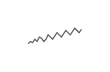
\begin{tikzpicture}[x=0.08em, y=0.08em, line width=0.4pt]
                \draw[FooterGray] (0,3) -- (1,4) -- (2,3.5) -- (3,5) -- (4,4) -- (5,6) -- (6,5.5) -- (7,4) -- (8,5) -- (9,7) -- (10,6) -- (11,5) -- (12,6.5) -- (13,8) -- (14,7) -- (15,6) -- (16,7.5) -- (17,9) -- (18,8) -- (19,7) -- (20,8.5) -- (21,10) -- (22,9) -- (23,8) -- (24,9.5);
            \end{tikzpicture}%
        }%
        \hskip0.5cm%
    }%
    \vskip6pt%
}

%=============================================================================
% PACKAGES
%=============================================================================
\usepackage[utf8]{inputenc}
\DeclareUnicodeCharacter{03B1}{\ensuremath{\alpha}}
\usepackage[T1]{fontenc}
\usepackage{amsmath, amssymb, amsthm}
\usepackage{mathtools}
\usepackage{bm}
\usepackage{tikz}
\usetikzlibrary{arrows.meta, positioning, shapes, calc, decorations.pathreplacing, shadings}
\usepackage{booktabs}
\usepackage{multirow}
\usepackage{array}
\usepackage{graphicx}
\usepackage{animate}
\usepackage{hyperref}
\usepackage{colortbl}
\usepackage{listings}
\lstset{language=Python, basicstyle=\ttfamily\scriptsize, keywordstyle=\color{MainBlue}\bfseries,
  commentstyle=\color{Forest}, stringstyle=\color{Crimson}, breaklines=true,
  frame=none, backgroundcolor=\color{VeryLightGray}, xleftmargin=2mm}
\hypersetup{colorlinks=true, linkcolor=MainBlue, urlcolor=MainBlue}
\graphicspath{{../../logos/}{../../charts/}{../../photos/}}
\usepackage{xcolor}
\hfuzz=2pt  % Suppress tiny overfull warnings (<2pt)
\vfuzz=2pt  % Suppress tiny vertical overfull warnings (<2pt)
% \mathrm in the sans-serif family of the slides (beamer resets \mathrm to the serif family at \begin{document};
% this hook runs after beamer's, so WN, Var, RMSE, ... in formulas match the surrounding text)
% Bold vectors and matrices in the same sans-serif family: \mathbf{A} in sans bold (beamer's own \mathbf came out in
% medium weight), and the bold upright Greek capitals of \boldsymbol / \bm (\bSigma, \bPhi, \boldsymbol{\Theta}) in
% cmss bold: bm.sty fixes its "boldoperators" font when it is loaded (serif cmbx), before beamer switches the
% operators to cmss, so it is reset here.
\AtBeginDocument{%
  \SetMathAlphabet{\mathrm}{normal}{\encodingdefault}{\sfdefault}{\mddefault}{n}%
  \SetMathAlphabet{\mathrm}{bold}{\encodingdefault}{\sfdefault}{bx}{n}%
  \SetMathAlphabet{\mathbf}{normal}{\encodingdefault}{\sfdefault}{bx}{n}%
  \SetMathAlphabet{\mathbf}{bold}{\encodingdefault}{\sfdefault}{bx}{n}%
  \SetSymbolFont{boldoperators}{normal}{OT1}{cmss}{bx}{n}%
  \SetSymbolFont{boldoperators}{bold}{OT1}{cmss}{bx}{n}}

%=============================================================================
% QUANTLET COMMANDS
%   \quantlet{<displayed name>}{<url>}       (generic, compatible with the older TSA decks)
%   \tsaquantlet{Ch_05}{TSA_ch5_garch}       -> https://github.com/danpele/Time-Series-Analysis/tree/main/Quantlets/Ch_05/TSA_ch5_garch
%   \qlurl{<folder>} is defined per chapter by the generator (Quantlets/Ch_NN/<folder>)
%=============================================================================
\newcommand{\tsarepo}{https://github.com/danpele/Time-Series-Analysis}
\newcommand{\tsaqlbase}{https://github.com/danpele/Time-Series-Analysis/tree/main/Quantlets}
\newcommand{\quantlet}[2]{%
    \hfill\href{#2}{%
        \raisebox{-0.15em}{
\includegraphics[height=0.7em]{ql_logo.png}}%
        \textcolor{MainBlue}{\tiny\ #1}%
    }%
}
\newcommand{\tsaquantlet}[2]{\quantlet{\detokenize{#2}}{\tsaqlbase/#1/#2}}

%=============================================================================
% NOTEBOOKS (Google Colab)
%   \colaburl{notebooks/EN/chapter5_seminar_notebook.ipynb} -> the Colab link of a file in the TSA repo
%   \nb: the chapter notebook (each seminar deck redefines it with \renewcommand)
%=============================================================================
\newcommand{\colaburl}[1]{https://colab.research.google.com/github/danpele/Time-Series-Analysis/blob/main/#1}
\newcommand{\nb}{https://colab.research.google.com/github/danpele/Time-Series-Analysis/tree/main/notebooks/EN}
\newcommand{\nbname}{notebooks/EN}

%=============================================================================
% SLIDE HELPERS (used by the generators; the same as in MFM)
%=============================================================================
% local font size for list bodies (the preamble forces \normalsize)
\newcommand{\itemsize}[1]{\setbeamertemplate{itemize/enumerate body begin}{#1}\setbeamertemplate{itemize/enumerate subbody begin}{#1}}
\newcommand{\intitle}[1]{{\hypersetup{urlcolor=white}#1}}   % white links inside coloured title bars
\newcommand{\imgcap}[1]{{\scriptsize #1}\\[0.5mm]}          % caption under a photo
\newcommand{\imgcredit}[2]{{\tiny\color{FooterGray}\href{#1}{#2}}}   % image credit: source URL, author/licence
\newcommand{\aiprompt}[1]{{\ttfamily\color{MainBlue}#1}}     % a prompt to an AI assistant

%=============================================================================
% SEMINARS: student version by default; the instructor wrapper *_solutions.tex sets \solutionstrue
%=============================================================================
\makeatletter\@ifundefined{ifsolutions}{\expandafter\newif\csname ifsolutions\endcsname}{}\makeatother
\newcommand{\solonly}[1]{\ifsolutions #1\fi}
\newcommand{\propsub}{\ifsolutions\else\framesubtitle{\ifdefined\tsalang Rezolvarea se discută la seminar\else Solution discussed in class\fi}\fi}

%=============================================================================
% APPENDIX AND CHAPTER LINKS (latex/appendix_links.py writes the calls; it also re-declares these
% macros before \begin{document}, so the decks compile with or without this preamble block)
%=============================================================================
\providecommand{\tsaapplink}[3]{\hypertarget{#2}{}\hyperlink{#1}{\beamergotobutton{#3}}}
\providecommand{\tsaappback}[2]{\begin{tikzpicture}[remember picture,overlay]\node[anchor=south east] at ([xshift=-3mm,yshift=7mm]current page.south east){\hyperlink{#1}{\beamerreturnbutton{#2}}};\end{tikzpicture}}
\providecommand{\tsachlink}[2]{\href{#1}{#2}}
\providecommand{\tsachlinkt}[2]{\href{#1}{\usebeamercolor[fg]{frametitle}#2}}

%=============================================================================
% QUANTINAR COMMAND: link către un curs Quantinar (subiecte avansate)
%=============================================================================
\newcommand{\quantinar}[2]{%
    \href{#2}{%
        \raisebox{-0.15em}{
\includegraphics[height=0.8em]{qr_logo.png}}%
        \textcolor{MainBlue}{\scriptsize\ #1}%
    }%
}

%=============================================================================
% CUSTOM TITLE PAGE
%=============================================================================
\defbeamertemplate*{title page}{hybrid}[1][]
{
    \vspace{0.2cm}
    % Logos row - top header (with clickable links)
    \begin{center}
        \href{https://www.ase.ro}{
\includegraphics[height=1.0cm]{ase_logo.png}}\hspace{0.3cm}%
        \href{https://theida.net}{
\includegraphics[height=1.0cm]{ida_logo.png}}\hspace{0.3cm}%
        \href{https://blockchain-research-center.com}{
\includegraphics[height=1.0cm]{brc_logo.png}}\hspace{0.3cm}%
        \href{https://www.ai4efin.ase.ro}{
\includegraphics[height=1.0cm]{ai4efin_logo.png}}\hspace{0.3cm}%
        \href{https://ipe.ro/new}{
\includegraphics[height=1.0cm]{acad_logo.png}}\hspace{0.3cm}%
        \href{https://www.digital-finance-msca.com}{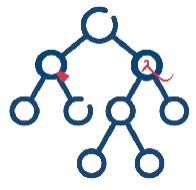
\includegraphics[height=1.0cm]{msca_logo.png}}%
    \end{center}

    \vspace{0.6cm}

    % Main title with Q logos on sides (with clickable links)
    \begin{center}
        \begin{minipage}{0.1\textwidth}
            \centering
            \href{https://quantlet.com}{
\includegraphics[height=1.1cm]{ql_logo.png}}
        \end{minipage}%
        \begin{minipage}{0.78\textwidth}
            \centering
            {\LARGE\bfseries\usebeamercolor[fg]{title}\inserttitle}

            \vspace{0.3cm}

            {\usebeamerfont{subtitle}\usebeamercolor[fg]{title}\insertsubtitle}
        \end{minipage}%
        \begin{minipage}{0.1\textwidth}
            \centering
            \href{https://quantinar.com}{
\includegraphics[height=1.1cm]{qr_logo.png}}
        \end{minipage}
    \end{center}

    \vspace{0.6cm}

    % Authors (left aligned)
    \hspace{0.5cm}{\usebeamerfont{author}\insertauthor}

    \vspace{0.3cm}

    % Institute/Affiliations (left aligned)
    \hspace{0.5cm}\begin{minipage}[t]{0.9\textwidth}
        \raggedright\small\insertinstitute
    \end{minipage}
}

%=============================================================================
% THEOREM ENVIRONMENTS
%=============================================================================
\theoremstyle{definition}
\setbeamertemplate{theorems}[numbered]
\ifdefined\tsalang
\newtheorem{defn}{Definiție}
\newtheorem{thm}{Teoremă}
\newtheorem{prop}{Propoziție}
\newtheorem{rmk}{Observație}
\else
\newtheorem{defn}{Definition}
\newtheorem{thm}{Theorem}
\newtheorem{prop}{Proposition}
\newtheorem{rmk}{Remark}
\fi

%=============================================================================
% CENTRED MINIPAGE (no extra vertical space)
%=============================================================================
\newenvironment{cminipage}[1]{%
    \par\noindent\hfill\begin{minipage}{#1}\ignorespaces
}{%
    \end{minipage}\hfill\null\par
}

%=============================================================================
% CUSTOM COMMANDS
%=============================================================================
\newcommand{\E}{\mathbb{E}}
\newcommand{\Var}{\text{Var}}
\newcommand{\Cov}{\text{Cov}}
\newcommand{\Corr}{\text{Corr}}
\newcommand{\R}{\mathbb{R}}
\newcommand{\N}{\mathbb{N}}
\newcommand{\Z}{\mathbb{Z}}
\newcommand{\B}{\mathbf{B}}
\newcommand{\imark}{\textcolor{MainBlue}{\textbullet}}
\newcommand{\RMSE}{\text{RMSE}}
\newcommand{\MAE}{\text{MAE}}
\newcommand{\MAPE}{\text{MAPE}}

% Boldface vector/matrix commands (VAR, VECM, state space; also used by the older TSA decks)
\newcommand{\bY}{\mathbf{Y}}
\newcommand{\bX}{\mathbf{X}}
\newcommand{\bA}{\mathbf{A}}
\newcommand{\bB}{\mathbf{B}}
\newcommand{\bepsilon}{\boldsymbol{\varepsilon}}
\newcommand{\bSigma}{\boldsymbol{\Sigma}}
\newcommand{\bPhi}{\boldsymbol{\Phi}}
\newcommand{\bGamma}{\boldsymbol{\Gamma}}
\newcommand{\bPi}{\boldsymbol{\Pi}}
\newcommand{\bc}{\mathbf{c}}
\newcommand{\balpha}{\boldsymbol{\alpha}}
\newcommand{\bbeta}{\boldsymbol{\beta}}
\newcommand{\bvarepsilon}{\boldsymbol{\varepsilon}}

% Legacy seminar marks (older TSA seminar decks)
\newcommand{\correct}{\textcolor{Forest}{\checkmark}}
\newcommand{\incorrect}{\textcolor{Crimson}{\texttimes}}
 se definește
%   \newcommand{\coursename}{Time Series Analysis}      (EN)
%   \newcommand{\coursename}{Serii de timp}       (RO)  și  \def\tsalang{ro}
% Fișierele .tex se află în EN/Courses, EN/Seminars, RO/Cursuri, RO/Seminarii (două niveluri sub rădăcină).
% Deck-urile sînt generate de latex/build_chapterN.py / build_seminarN.py (vezi latex/tsa_build.py).

\documentclass[9pt, aspectratio=169, t]{beamer}
\providecommand{\coursename}{Time Series Analysis}

% Ensure content fits on slides
\setbeamersize{text margin left=8mm, text margin right=8mm}
% Smaller institute font (title page)
\setbeamerfont{institute}{size=\footnotesize}

%=============================================================================
% THEME AND STYLE CONFIGURATION
%=============================================================================
\usetheme{default}
% Using default theme for clean header/footer control

% Color Palette (matching Redispatch PDF)
\definecolor{MainBlue}{RGB}{26, 58, 110}
\definecolor{AccentBlue}{RGB}{26, 58, 110}
\definecolor{IDAred}{RGB}{205, 0, 0}
\definecolor{DarkGray}{RGB}{51, 51, 51}
\definecolor{MediumGray}{RGB}{128, 128, 128}
\definecolor{LightGray}{RGB}{248, 248, 248}
\definecolor{VeryLightGray}{RGB}{235, 235, 235}
\definecolor{KeynoteGray}{RGB}{218, 218, 218}
\definecolor{SectionGray}{RGB}{120, 120, 120}
\definecolor{FooterGray}{RGB}{100, 100, 100}
\definecolor{Crimson}{RGB}{220, 53, 69}
\definecolor{Forest}{RGB}{46, 125, 50}
\definecolor{Amber}{RGB}{181, 133, 63}
\definecolor{Orange}{RGB}{230, 126, 34}
\definecolor{Purple}{RGB}{142, 68, 173}

% Gradient background (exact Keynote 315° gradient: white to RGB 218,218,218)
\setbeamertemplate{background}{%
    \begin{tikzpicture}[remember picture, overlay]
        \shade[shading=axis, shading angle=315,
        top color=white, bottom color=KeynoteGray]
        (current page.south west) rectangle (current page.north east);
    \end{tikzpicture}%
}
% Fallback solid color for compatibility
\setbeamercolor{background canvas}{bg=}

\setbeamercolor{palette primary}{bg=MainBlue, fg=white}
\setbeamercolor{palette secondary}{bg=MainBlue!85, fg=white}
\setbeamercolor{palette tertiary}{bg=MainBlue!70, fg=white}
\setbeamercolor{structure}{fg=MainBlue}
\setbeamercolor{title}{fg=IDAred}
\setbeamercolor{frametitle}{fg=IDAred, bg=}
\setbeamercolor{block title}{bg=MainBlue, fg=white}
\setbeamercolor{block body}{bg=VeryLightGray, fg=DarkGray}
\setbeamercolor{block title alerted}{bg=Crimson, fg=white}
\setbeamercolor{block body alerted}{bg=Crimson!8, fg=DarkGray}
\setbeamercolor{block title example}{bg=Forest, fg=white}
\setbeamercolor{block body example}{bg=Forest!8, fg=DarkGray}
\setbeamercolor{item}{fg=MainBlue}

% Footer colors (override Madrid theme blue)
\setbeamercolor{author in head/foot}{fg=FooterGray, bg=}
\setbeamercolor{title in head/foot}{fg=FooterGray, bg=}
\setbeamercolor{date in head/foot}{fg=FooterGray, bg=}
\setbeamercolor{section in head/foot}{fg=FooterGray, bg=}
\setbeamercolor{subsection in head/foot}{fg=FooterGray, bg=}

% Bullet styles (apply everywhere including blocks)
\setbeamertemplate{itemize item}{\color{MainBlue}$\boxdot$}
\setbeamertemplate{itemize subitem}{\color{MainBlue}$\blacktriangleright$}
\setbeamertemplate{itemize subsubitem}{\color{MainBlue}\tiny$\bullet$}
\setbeamertemplate{itemize/enumerate body begin}{\normalsize}
\setbeamertemplate{itemize/enumerate subbody begin}{\normalsize}

% Item spacing - compact style
\setlength{\leftmargini}{10pt}       % Level 1: minimal indent
\setlength{\leftmarginii}{10pt}      % Level 2: minimal additional indent
% Compact list spacing (zero extra space before/after lists in blocks)
\makeatletter
\def\@listi{\leftmargin\leftmargini \topsep 0pt \parsep 0pt \itemsep 0pt}
\def\@listii{\leftmargin\leftmarginii \topsep 0pt \parsep 0pt \itemsep 0pt}
\makeatother

\setbeamertemplate{navigation symbols}{}

%=============================================================================
% CUSTOM HEADLINE
%=============================================================================
\setbeamertemplate{headline}{%
    \vskip10pt%
    \hbox to \paperwidth{%
        \hskip0.5cm%
        {\small\color{FooterGray}\renewcommand{\hyperlink}[2]{##2}\insertsectionhead}%
        \hfill%
        \textcolor{FooterGray}{\small\insertframenumber}%
        \hskip0.5cm%
    }%
    \vskip4pt%
    {\color{FooterGray}\hrule height 0.4pt}%
}

%=============================================================================
% CUSTOM FOOTER
%=============================================================================
\usepackage{fontawesome5}

\setbeamertemplate{footline}{%
    {\color{FooterGray}\hrule height 0.4pt}%
    \vskip4pt%
    \hbox to \paperwidth{%
        \hskip0.5cm%
        \textcolor{FooterGray}{\small\coursename}%
        \hfill%
        \raisebox{-0.1em}{%
            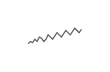
\begin{tikzpicture}[x=0.08em, y=0.08em, line width=0.4pt]
                \draw[FooterGray] (0,3) -- (1,4) -- (2,3.5) -- (3,5) -- (4,4) -- (5,6) -- (6,5.5) -- (7,4) -- (8,5) -- (9,7) -- (10,6) -- (11,5) -- (12,6.5) -- (13,8) -- (14,7) -- (15,6) -- (16,7.5) -- (17,9) -- (18,8) -- (19,7) -- (20,8.5) -- (21,10) -- (22,9) -- (23,8) -- (24,9.5);
            \end{tikzpicture}%
        }%
        \hskip0.5cm%
    }%
    \vskip6pt%
}

%=============================================================================
% PACKAGES
%=============================================================================
\usepackage[utf8]{inputenc}
\DeclareUnicodeCharacter{03B1}{\ensuremath{\alpha}}
\usepackage[T1]{fontenc}
\usepackage{amsmath, amssymb, amsthm}
\usepackage{mathtools}
\usepackage{bm}
\usepackage{tikz}
\usetikzlibrary{arrows.meta, positioning, shapes, calc, decorations.pathreplacing, shadings}
\usepackage{booktabs}
\usepackage{multirow}
\usepackage{array}
\usepackage{graphicx}
\usepackage{animate}
\usepackage{hyperref}
\usepackage{colortbl}
\usepackage{listings}
\lstset{language=Python, basicstyle=\ttfamily\scriptsize, keywordstyle=\color{MainBlue}\bfseries,
  commentstyle=\color{Forest}, stringstyle=\color{Crimson}, breaklines=true,
  frame=none, backgroundcolor=\color{VeryLightGray}, xleftmargin=2mm}
\hypersetup{colorlinks=true, linkcolor=MainBlue, urlcolor=MainBlue}
\graphicspath{{../../logos/}{../../charts/}{../../photos/}}
\usepackage{xcolor}
\hfuzz=2pt  % Suppress tiny overfull warnings (<2pt)
\vfuzz=2pt  % Suppress tiny vertical overfull warnings (<2pt)
% \mathrm in the sans-serif family of the slides (beamer resets \mathrm to the serif family at \begin{document};
% this hook runs after beamer's, so WN, Var, RMSE, ... in formulas match the surrounding text)
% Bold vectors and matrices in the same sans-serif family: \mathbf{A} in sans bold (beamer's own \mathbf came out in
% medium weight), and the bold upright Greek capitals of \boldsymbol / \bm (\bSigma, \bPhi, \boldsymbol{\Theta}) in
% cmss bold: bm.sty fixes its "boldoperators" font when it is loaded (serif cmbx), before beamer switches the
% operators to cmss, so it is reset here.
\AtBeginDocument{%
  \SetMathAlphabet{\mathrm}{normal}{\encodingdefault}{\sfdefault}{\mddefault}{n}%
  \SetMathAlphabet{\mathrm}{bold}{\encodingdefault}{\sfdefault}{bx}{n}%
  \SetMathAlphabet{\mathbf}{normal}{\encodingdefault}{\sfdefault}{bx}{n}%
  \SetMathAlphabet{\mathbf}{bold}{\encodingdefault}{\sfdefault}{bx}{n}%
  \SetSymbolFont{boldoperators}{normal}{OT1}{cmss}{bx}{n}%
  \SetSymbolFont{boldoperators}{bold}{OT1}{cmss}{bx}{n}}

%=============================================================================
% QUANTLET COMMANDS
%   \quantlet{<displayed name>}{<url>}       (generic, compatible with the older TSA decks)
%   \tsaquantlet{Ch_05}{TSA_ch5_garch}       -> https://github.com/danpele/Time-Series-Analysis/tree/main/Quantlets/Ch_05/TSA_ch5_garch
%   \qlurl{<folder>} is defined per chapter by the generator (Quantlets/Ch_NN/<folder>)
%=============================================================================
\newcommand{\tsarepo}{https://github.com/danpele/Time-Series-Analysis}
\newcommand{\tsaqlbase}{https://github.com/danpele/Time-Series-Analysis/tree/main/Quantlets}
\newcommand{\quantlet}[2]{%
    \hfill\href{#2}{%
        \raisebox{-0.15em}{
\includegraphics[height=0.7em]{ql_logo.png}}%
        \textcolor{MainBlue}{\tiny\ #1}%
    }%
}
\newcommand{\tsaquantlet}[2]{\quantlet{\detokenize{#2}}{\tsaqlbase/#1/#2}}

%=============================================================================
% NOTEBOOKS (Google Colab)
%   \colaburl{notebooks/EN/chapter5_seminar_notebook.ipynb} -> the Colab link of a file in the TSA repo
%   \nb: the chapter notebook (each seminar deck redefines it with \renewcommand)
%=============================================================================
\newcommand{\colaburl}[1]{https://colab.research.google.com/github/danpele/Time-Series-Analysis/blob/main/#1}
\newcommand{\nb}{https://colab.research.google.com/github/danpele/Time-Series-Analysis/tree/main/notebooks/EN}
\newcommand{\nbname}{notebooks/EN}

%=============================================================================
% SLIDE HELPERS (used by the generators; the same as in MFM)
%=============================================================================
% local font size for list bodies (the preamble forces \normalsize)
\newcommand{\itemsize}[1]{\setbeamertemplate{itemize/enumerate body begin}{#1}\setbeamertemplate{itemize/enumerate subbody begin}{#1}}
\newcommand{\intitle}[1]{{\hypersetup{urlcolor=white}#1}}   % white links inside coloured title bars
\newcommand{\imgcap}[1]{{\scriptsize #1}\\[0.5mm]}          % caption under a photo
\newcommand{\imgcredit}[2]{{\tiny\color{FooterGray}\href{#1}{#2}}}   % image credit: source URL, author/licence
\newcommand{\aiprompt}[1]{{\ttfamily\color{MainBlue}#1}}     % a prompt to an AI assistant

%=============================================================================
% SEMINARS: student version by default; the instructor wrapper *_solutions.tex sets \solutionstrue
%=============================================================================
\makeatletter\@ifundefined{ifsolutions}{\expandafter\newif\csname ifsolutions\endcsname}{}\makeatother
\newcommand{\solonly}[1]{\ifsolutions #1\fi}
\newcommand{\propsub}{\ifsolutions\else\framesubtitle{\ifdefined\tsalang Rezolvarea se discută la seminar\else Solution discussed in class\fi}\fi}

%=============================================================================
% APPENDIX AND CHAPTER LINKS (latex/appendix_links.py writes the calls; it also re-declares these
% macros before \begin{document}, so the decks compile with or without this preamble block)
%=============================================================================
\providecommand{\tsaapplink}[3]{\hypertarget{#2}{}\hyperlink{#1}{\beamergotobutton{#3}}}
\providecommand{\tsaappback}[2]{\begin{tikzpicture}[remember picture,overlay]\node[anchor=south east] at ([xshift=-3mm,yshift=7mm]current page.south east){\hyperlink{#1}{\beamerreturnbutton{#2}}};\end{tikzpicture}}
\providecommand{\tsachlink}[2]{\href{#1}{#2}}
\providecommand{\tsachlinkt}[2]{\href{#1}{\usebeamercolor[fg]{frametitle}#2}}

%=============================================================================
% QUANTINAR COMMAND: link către un curs Quantinar (subiecte avansate)
%=============================================================================
\newcommand{\quantinar}[2]{%
    \href{#2}{%
        \raisebox{-0.15em}{
\includegraphics[height=0.8em]{qr_logo.png}}%
        \textcolor{MainBlue}{\scriptsize\ #1}%
    }%
}

%=============================================================================
% CUSTOM TITLE PAGE
%=============================================================================
\defbeamertemplate*{title page}{hybrid}[1][]
{
    \vspace{0.2cm}
    % Logos row - top header (with clickable links)
    \begin{center}
        \href{https://www.ase.ro}{
\includegraphics[height=1.0cm]{ase_logo.png}}\hspace{0.3cm}%
        \href{https://theida.net}{
\includegraphics[height=1.0cm]{ida_logo.png}}\hspace{0.3cm}%
        \href{https://blockchain-research-center.com}{
\includegraphics[height=1.0cm]{brc_logo.png}}\hspace{0.3cm}%
        \href{https://www.ai4efin.ase.ro}{
\includegraphics[height=1.0cm]{ai4efin_logo.png}}\hspace{0.3cm}%
        \href{https://ipe.ro/new}{
\includegraphics[height=1.0cm]{acad_logo.png}}\hspace{0.3cm}%
        \href{https://www.digital-finance-msca.com}{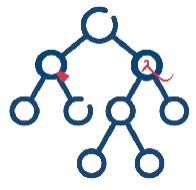
\includegraphics[height=1.0cm]{msca_logo.png}}%
    \end{center}

    \vspace{0.6cm}

    % Main title with Q logos on sides (with clickable links)
    \begin{center}
        \begin{minipage}{0.1\textwidth}
            \centering
            \href{https://quantlet.com}{
\includegraphics[height=1.1cm]{ql_logo.png}}
        \end{minipage}%
        \begin{minipage}{0.78\textwidth}
            \centering
            {\LARGE\bfseries\usebeamercolor[fg]{title}\inserttitle}

            \vspace{0.3cm}

            {\usebeamerfont{subtitle}\usebeamercolor[fg]{title}\insertsubtitle}
        \end{minipage}%
        \begin{minipage}{0.1\textwidth}
            \centering
            \href{https://quantinar.com}{
\includegraphics[height=1.1cm]{qr_logo.png}}
        \end{minipage}
    \end{center}

    \vspace{0.6cm}

    % Authors (left aligned)
    \hspace{0.5cm}{\usebeamerfont{author}\insertauthor}

    \vspace{0.3cm}

    % Institute/Affiliations (left aligned)
    \hspace{0.5cm}\begin{minipage}[t]{0.9\textwidth}
        \raggedright\small\insertinstitute
    \end{minipage}
}

%=============================================================================
% THEOREM ENVIRONMENTS
%=============================================================================
\theoremstyle{definition}
\setbeamertemplate{theorems}[numbered]
\ifdefined\tsalang
\newtheorem{defn}{Definiție}
\newtheorem{thm}{Teoremă}
\newtheorem{prop}{Propoziție}
\newtheorem{rmk}{Observație}
\else
\newtheorem{defn}{Definition}
\newtheorem{thm}{Theorem}
\newtheorem{prop}{Proposition}
\newtheorem{rmk}{Remark}
\fi

%=============================================================================
% CENTRED MINIPAGE (no extra vertical space)
%=============================================================================
\newenvironment{cminipage}[1]{%
    \par\noindent\hfill\begin{minipage}{#1}\ignorespaces
}{%
    \end{minipage}\hfill\null\par
}

%=============================================================================
% CUSTOM COMMANDS
%=============================================================================
\newcommand{\E}{\mathbb{E}}
\newcommand{\Var}{\text{Var}}
\newcommand{\Cov}{\text{Cov}}
\newcommand{\Corr}{\text{Corr}}
\newcommand{\R}{\mathbb{R}}
\newcommand{\N}{\mathbb{N}}
\newcommand{\Z}{\mathbb{Z}}
\newcommand{\B}{\mathbf{B}}
\newcommand{\imark}{\textcolor{MainBlue}{\textbullet}}
\newcommand{\RMSE}{\text{RMSE}}
\newcommand{\MAE}{\text{MAE}}
\newcommand{\MAPE}{\text{MAPE}}

% Boldface vector/matrix commands (VAR, VECM, state space; also used by the older TSA decks)
\newcommand{\bY}{\mathbf{Y}}
\newcommand{\bX}{\mathbf{X}}
\newcommand{\bA}{\mathbf{A}}
\newcommand{\bB}{\mathbf{B}}
\newcommand{\bepsilon}{\boldsymbol{\varepsilon}}
\newcommand{\bSigma}{\boldsymbol{\Sigma}}
\newcommand{\bPhi}{\boldsymbol{\Phi}}
\newcommand{\bGamma}{\boldsymbol{\Gamma}}
\newcommand{\bPi}{\boldsymbol{\Pi}}
\newcommand{\bc}{\mathbf{c}}
\newcommand{\balpha}{\boldsymbol{\alpha}}
\newcommand{\bbeta}{\boldsymbol{\beta}}
\newcommand{\bvarepsilon}{\boldsymbol{\varepsilon}}

% Legacy seminar marks (older TSA seminar decks)
\newcommand{\correct}{\textcolor{Forest}{\checkmark}}
\newcommand{\incorrect}{\textcolor{Crimson}{\texttimes}}
 se definește
%   \newcommand{\coursename}{Time Series Analysis}      (EN)
%   \newcommand{\coursename}{Serii de timp}       (RO)  și  \def\tsalang{ro}
% Fișierele .tex se află în EN/Courses, EN/Seminars, RO/Cursuri, RO/Seminarii (două niveluri sub rădăcină).
% Deck-urile sînt generate de latex/build_chapterN.py / build_seminarN.py (vezi latex/tsa_build.py).

\documentclass[9pt, aspectratio=169, t]{beamer}
\providecommand{\coursename}{Time Series Analysis}

% Ensure content fits on slides
\setbeamersize{text margin left=8mm, text margin right=8mm}
% Smaller institute font (title page)
\setbeamerfont{institute}{size=\footnotesize}

%=============================================================================
% THEME AND STYLE CONFIGURATION
%=============================================================================
\usetheme{default}
% Using default theme for clean header/footer control

% Color Palette (matching Redispatch PDF)
\definecolor{MainBlue}{RGB}{26, 58, 110}
\definecolor{AccentBlue}{RGB}{26, 58, 110}
\definecolor{IDAred}{RGB}{205, 0, 0}
\definecolor{DarkGray}{RGB}{51, 51, 51}
\definecolor{MediumGray}{RGB}{128, 128, 128}
\definecolor{LightGray}{RGB}{248, 248, 248}
\definecolor{VeryLightGray}{RGB}{235, 235, 235}
\definecolor{KeynoteGray}{RGB}{218, 218, 218}
\definecolor{SectionGray}{RGB}{120, 120, 120}
\definecolor{FooterGray}{RGB}{100, 100, 100}
\definecolor{Crimson}{RGB}{220, 53, 69}
\definecolor{Forest}{RGB}{46, 125, 50}
\definecolor{Amber}{RGB}{181, 133, 63}
\definecolor{Orange}{RGB}{230, 126, 34}
\definecolor{Purple}{RGB}{142, 68, 173}

% Gradient background (exact Keynote 315° gradient: white to RGB 218,218,218)
\setbeamertemplate{background}{%
    \begin{tikzpicture}[remember picture, overlay]
        \shade[shading=axis, shading angle=315,
        top color=white, bottom color=KeynoteGray]
        (current page.south west) rectangle (current page.north east);
    \end{tikzpicture}%
}
% Fallback solid color for compatibility
\setbeamercolor{background canvas}{bg=}

\setbeamercolor{palette primary}{bg=MainBlue, fg=white}
\setbeamercolor{palette secondary}{bg=MainBlue!85, fg=white}
\setbeamercolor{palette tertiary}{bg=MainBlue!70, fg=white}
\setbeamercolor{structure}{fg=MainBlue}
\setbeamercolor{title}{fg=IDAred}
\setbeamercolor{frametitle}{fg=IDAred, bg=}
\setbeamercolor{block title}{bg=MainBlue, fg=white}
\setbeamercolor{block body}{bg=VeryLightGray, fg=DarkGray}
\setbeamercolor{block title alerted}{bg=Crimson, fg=white}
\setbeamercolor{block body alerted}{bg=Crimson!8, fg=DarkGray}
\setbeamercolor{block title example}{bg=Forest, fg=white}
\setbeamercolor{block body example}{bg=Forest!8, fg=DarkGray}
\setbeamercolor{item}{fg=MainBlue}

% Footer colors (override Madrid theme blue)
\setbeamercolor{author in head/foot}{fg=FooterGray, bg=}
\setbeamercolor{title in head/foot}{fg=FooterGray, bg=}
\setbeamercolor{date in head/foot}{fg=FooterGray, bg=}
\setbeamercolor{section in head/foot}{fg=FooterGray, bg=}
\setbeamercolor{subsection in head/foot}{fg=FooterGray, bg=}

% Bullet styles (apply everywhere including blocks)
\setbeamertemplate{itemize item}{\color{MainBlue}$\boxdot$}
\setbeamertemplate{itemize subitem}{\color{MainBlue}$\blacktriangleright$}
\setbeamertemplate{itemize subsubitem}{\color{MainBlue}\tiny$\bullet$}
\setbeamertemplate{itemize/enumerate body begin}{\normalsize}
\setbeamertemplate{itemize/enumerate subbody begin}{\normalsize}

% Item spacing - compact style
\setlength{\leftmargini}{10pt}       % Level 1: minimal indent
\setlength{\leftmarginii}{10pt}      % Level 2: minimal additional indent
% Compact list spacing (zero extra space before/after lists in blocks)
\makeatletter
\def\@listi{\leftmargin\leftmargini \topsep 0pt \parsep 0pt \itemsep 0pt}
\def\@listii{\leftmargin\leftmarginii \topsep 0pt \parsep 0pt \itemsep 0pt}
\makeatother

\setbeamertemplate{navigation symbols}{}

%=============================================================================
% CUSTOM HEADLINE
%=============================================================================
\setbeamertemplate{headline}{%
    \vskip10pt%
    \hbox to \paperwidth{%
        \hskip0.5cm%
        {\small\color{FooterGray}\renewcommand{\hyperlink}[2]{##2}\insertsectionhead}%
        \hfill%
        \textcolor{FooterGray}{\small\insertframenumber}%
        \hskip0.5cm%
    }%
    \vskip4pt%
    {\color{FooterGray}\hrule height 0.4pt}%
}

%=============================================================================
% CUSTOM FOOTER
%=============================================================================
\usepackage{fontawesome5}

\setbeamertemplate{footline}{%
    {\color{FooterGray}\hrule height 0.4pt}%
    \vskip4pt%
    \hbox to \paperwidth{%
        \hskip0.5cm%
        \textcolor{FooterGray}{\small\coursename}%
        \hfill%
        \raisebox{-0.1em}{%
            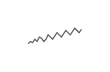
\begin{tikzpicture}[x=0.08em, y=0.08em, line width=0.4pt]
                \draw[FooterGray] (0,3) -- (1,4) -- (2,3.5) -- (3,5) -- (4,4) -- (5,6) -- (6,5.5) -- (7,4) -- (8,5) -- (9,7) -- (10,6) -- (11,5) -- (12,6.5) -- (13,8) -- (14,7) -- (15,6) -- (16,7.5) -- (17,9) -- (18,8) -- (19,7) -- (20,8.5) -- (21,10) -- (22,9) -- (23,8) -- (24,9.5);
            \end{tikzpicture}%
        }%
        \hskip0.5cm%
    }%
    \vskip6pt%
}

%=============================================================================
% PACKAGES
%=============================================================================
\usepackage[utf8]{inputenc}
\DeclareUnicodeCharacter{03B1}{\ensuremath{\alpha}}
\usepackage[T1]{fontenc}
\usepackage{amsmath, amssymb, amsthm}
\usepackage{mathtools}
\usepackage{bm}
\usepackage{tikz}
\usetikzlibrary{arrows.meta, positioning, shapes, calc, decorations.pathreplacing, shadings}
\usepackage{booktabs}
\usepackage{multirow}
\usepackage{array}
\usepackage{graphicx}
\usepackage{animate}
\usepackage{hyperref}
\usepackage{colortbl}
\usepackage{listings}
\lstset{language=Python, basicstyle=\ttfamily\scriptsize, keywordstyle=\color{MainBlue}\bfseries,
  commentstyle=\color{Forest}, stringstyle=\color{Crimson}, breaklines=true,
  frame=none, backgroundcolor=\color{VeryLightGray}, xleftmargin=2mm}
\hypersetup{colorlinks=true, linkcolor=MainBlue, urlcolor=MainBlue}
\graphicspath{{../../logos/}{../../charts/}{../../photos/}}
\usepackage{xcolor}
\hfuzz=2pt  % Suppress tiny overfull warnings (<2pt)
\vfuzz=2pt  % Suppress tiny vertical overfull warnings (<2pt)
% \mathrm in the sans-serif family of the slides (beamer resets \mathrm to the serif family at \begin{document};
% this hook runs after beamer's, so WN, Var, RMSE, ... in formulas match the surrounding text)
% Bold vectors and matrices in the same sans-serif family: \mathbf{A} in sans bold (beamer's own \mathbf came out in
% medium weight), and the bold upright Greek capitals of \boldsymbol / \bm (\bSigma, \bPhi, \boldsymbol{\Theta}) in
% cmss bold: bm.sty fixes its "boldoperators" font when it is loaded (serif cmbx), before beamer switches the
% operators to cmss, so it is reset here.
\AtBeginDocument{%
  \SetMathAlphabet{\mathrm}{normal}{\encodingdefault}{\sfdefault}{\mddefault}{n}%
  \SetMathAlphabet{\mathrm}{bold}{\encodingdefault}{\sfdefault}{bx}{n}%
  \SetMathAlphabet{\mathbf}{normal}{\encodingdefault}{\sfdefault}{bx}{n}%
  \SetMathAlphabet{\mathbf}{bold}{\encodingdefault}{\sfdefault}{bx}{n}%
  \SetSymbolFont{boldoperators}{normal}{OT1}{cmss}{bx}{n}%
  \SetSymbolFont{boldoperators}{bold}{OT1}{cmss}{bx}{n}}

%=============================================================================
% QUANTLET COMMANDS
%   \quantlet{<displayed name>}{<url>}       (generic, compatible with the older TSA decks)
%   \tsaquantlet{Ch_05}{TSA_ch5_garch}       -> https://github.com/danpele/Time-Series-Analysis/tree/main/Quantlets/Ch_05/TSA_ch5_garch
%   \qlurl{<folder>} is defined per chapter by the generator (Quantlets/Ch_NN/<folder>)
%=============================================================================
\newcommand{\tsarepo}{https://github.com/danpele/Time-Series-Analysis}
\newcommand{\tsaqlbase}{https://github.com/danpele/Time-Series-Analysis/tree/main/Quantlets}
\newcommand{\quantlet}[2]{%
    \hfill\href{#2}{%
        \raisebox{-0.15em}{
\includegraphics[height=0.7em]{ql_logo.png}}%
        \textcolor{MainBlue}{\tiny\ #1}%
    }%
}
\newcommand{\tsaquantlet}[2]{\quantlet{\detokenize{#2}}{\tsaqlbase/#1/#2}}

%=============================================================================
% NOTEBOOKS (Google Colab)
%   \colaburl{notebooks/EN/chapter5_seminar_notebook.ipynb} -> the Colab link of a file in the TSA repo
%   \nb: the chapter notebook (each seminar deck redefines it with \renewcommand)
%=============================================================================
\newcommand{\colaburl}[1]{https://colab.research.google.com/github/danpele/Time-Series-Analysis/blob/main/#1}
\newcommand{\nb}{https://colab.research.google.com/github/danpele/Time-Series-Analysis/tree/main/notebooks/EN}
\newcommand{\nbname}{notebooks/EN}

%=============================================================================
% SLIDE HELPERS (used by the generators; the same as in MFM)
%=============================================================================
% local font size for list bodies (the preamble forces \normalsize)
\newcommand{\itemsize}[1]{\setbeamertemplate{itemize/enumerate body begin}{#1}\setbeamertemplate{itemize/enumerate subbody begin}{#1}}
\newcommand{\intitle}[1]{{\hypersetup{urlcolor=white}#1}}   % white links inside coloured title bars
\newcommand{\imgcap}[1]{{\scriptsize #1}\\[0.5mm]}          % caption under a photo
\newcommand{\imgcredit}[2]{{\tiny\color{FooterGray}\href{#1}{#2}}}   % image credit: source URL, author/licence
\newcommand{\aiprompt}[1]{{\ttfamily\color{MainBlue}#1}}     % a prompt to an AI assistant

%=============================================================================
% SEMINARS: student version by default; the instructor wrapper *_solutions.tex sets \solutionstrue
%=============================================================================
\makeatletter\@ifundefined{ifsolutions}{\expandafter\newif\csname ifsolutions\endcsname}{}\makeatother
\newcommand{\solonly}[1]{\ifsolutions #1\fi}
\newcommand{\propsub}{\ifsolutions\else\framesubtitle{\ifdefined\tsalang Rezolvarea se discută la seminar\else Solution discussed in class\fi}\fi}

%=============================================================================
% APPENDIX AND CHAPTER LINKS (latex/appendix_links.py writes the calls; it also re-declares these
% macros before \begin{document}, so the decks compile with or without this preamble block)
%=============================================================================
\providecommand{\tsaapplink}[3]{\hypertarget{#2}{}\hyperlink{#1}{\beamergotobutton{#3}}}
\providecommand{\tsaappback}[2]{\begin{tikzpicture}[remember picture,overlay]\node[anchor=south east] at ([xshift=-3mm,yshift=7mm]current page.south east){\hyperlink{#1}{\beamerreturnbutton{#2}}};\end{tikzpicture}}
\providecommand{\tsachlink}[2]{\href{#1}{#2}}
\providecommand{\tsachlinkt}[2]{\href{#1}{\usebeamercolor[fg]{frametitle}#2}}

%=============================================================================
% QUANTINAR COMMAND: link către un curs Quantinar (subiecte avansate)
%=============================================================================
\newcommand{\quantinar}[2]{%
    \href{#2}{%
        \raisebox{-0.15em}{
\includegraphics[height=0.8em]{qr_logo.png}}%
        \textcolor{MainBlue}{\scriptsize\ #1}%
    }%
}

%=============================================================================
% CUSTOM TITLE PAGE
%=============================================================================
\defbeamertemplate*{title page}{hybrid}[1][]
{
    \vspace{0.2cm}
    % Logos row - top header (with clickable links)
    \begin{center}
        \href{https://www.ase.ro}{
\includegraphics[height=1.0cm]{ase_logo.png}}\hspace{0.3cm}%
        \href{https://theida.net}{
\includegraphics[height=1.0cm]{ida_logo.png}}\hspace{0.3cm}%
        \href{https://blockchain-research-center.com}{
\includegraphics[height=1.0cm]{brc_logo.png}}\hspace{0.3cm}%
        \href{https://www.ai4efin.ase.ro}{
\includegraphics[height=1.0cm]{ai4efin_logo.png}}\hspace{0.3cm}%
        \href{https://ipe.ro/new}{
\includegraphics[height=1.0cm]{acad_logo.png}}\hspace{0.3cm}%
        \href{https://www.digital-finance-msca.com}{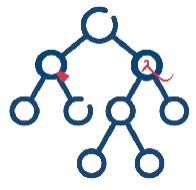
\includegraphics[height=1.0cm]{msca_logo.png}}%
    \end{center}

    \vspace{0.6cm}

    % Main title with Q logos on sides (with clickable links)
    \begin{center}
        \begin{minipage}{0.1\textwidth}
            \centering
            \href{https://quantlet.com}{
\includegraphics[height=1.1cm]{ql_logo.png}}
        \end{minipage}%
        \begin{minipage}{0.78\textwidth}
            \centering
            {\LARGE\bfseries\usebeamercolor[fg]{title}\inserttitle}

            \vspace{0.3cm}

            {\usebeamerfont{subtitle}\usebeamercolor[fg]{title}\insertsubtitle}
        \end{minipage}%
        \begin{minipage}{0.1\textwidth}
            \centering
            \href{https://quantinar.com}{
\includegraphics[height=1.1cm]{qr_logo.png}}
        \end{minipage}
    \end{center}

    \vspace{0.6cm}

    % Authors (left aligned)
    \hspace{0.5cm}{\usebeamerfont{author}\insertauthor}

    \vspace{0.3cm}

    % Institute/Affiliations (left aligned)
    \hspace{0.5cm}\begin{minipage}[t]{0.9\textwidth}
        \raggedright\small\insertinstitute
    \end{minipage}
}

%=============================================================================
% THEOREM ENVIRONMENTS
%=============================================================================
\theoremstyle{definition}
\setbeamertemplate{theorems}[numbered]
\ifdefined\tsalang
\newtheorem{defn}{Definiție}
\newtheorem{thm}{Teoremă}
\newtheorem{prop}{Propoziție}
\newtheorem{rmk}{Observație}
\else
\newtheorem{defn}{Definition}
\newtheorem{thm}{Theorem}
\newtheorem{prop}{Proposition}
\newtheorem{rmk}{Remark}
\fi

%=============================================================================
% CENTRED MINIPAGE (no extra vertical space)
%=============================================================================
\newenvironment{cminipage}[1]{%
    \par\noindent\hfill\begin{minipage}{#1}\ignorespaces
}{%
    \end{minipage}\hfill\null\par
}

%=============================================================================
% CUSTOM COMMANDS
%=============================================================================
\newcommand{\E}{\mathbb{E}}
\newcommand{\Var}{\text{Var}}
\newcommand{\Cov}{\text{Cov}}
\newcommand{\Corr}{\text{Corr}}
\newcommand{\R}{\mathbb{R}}
\newcommand{\N}{\mathbb{N}}
\newcommand{\Z}{\mathbb{Z}}
\newcommand{\B}{\mathbf{B}}
\newcommand{\imark}{\textcolor{MainBlue}{\textbullet}}
\newcommand{\RMSE}{\text{RMSE}}
\newcommand{\MAE}{\text{MAE}}
\newcommand{\MAPE}{\text{MAPE}}

% Boldface vector/matrix commands (VAR, VECM, state space; also used by the older TSA decks)
\newcommand{\bY}{\mathbf{Y}}
\newcommand{\bX}{\mathbf{X}}
\newcommand{\bA}{\mathbf{A}}
\newcommand{\bB}{\mathbf{B}}
\newcommand{\bepsilon}{\boldsymbol{\varepsilon}}
\newcommand{\bSigma}{\boldsymbol{\Sigma}}
\newcommand{\bPhi}{\boldsymbol{\Phi}}
\newcommand{\bGamma}{\boldsymbol{\Gamma}}
\newcommand{\bPi}{\boldsymbol{\Pi}}
\newcommand{\bc}{\mathbf{c}}
\newcommand{\balpha}{\boldsymbol{\alpha}}
\newcommand{\bbeta}{\boldsymbol{\beta}}
\newcommand{\bvarepsilon}{\boldsymbol{\varepsilon}}

% Legacy seminar marks (older TSA seminar decks)
\newcommand{\correct}{\textcolor{Forest}{\checkmark}}
\newcommand{\incorrect}{\textcolor{Crimson}{\texttimes}}


\newcommand{\qlurl}[1]{https://github.com/danpele/Time-Series-Analysis/tree/main/Quantlets/Ch_08/#1}

% Clickable citations (DOIs verified via Crossref)
\newcommand{\refHP}{\href{https://doi.org/10.1007/978-3-031-13584-2}{Huang and Petukhina (2022)}}
\newcommand{\refBDtm}{\href{https://doi.org/10.1007/978-1-4419-0320-4}{Brockwell and Davis (1991)}}
\newcommand{\refBeran}{\href{https://doi.org/10.1007/978-3-642-35512-7}{Beran et al.\ (2013)}}
\newcommand{\refBaillie}{\href{https://doi.org/10.1016/0304-4076(95)01732-1}{Baillie (1996)}}
\newcommand{\refGraves}{\href{https://doi.org/10.3390/e19090437}{Graves et al.\ (2017)}}
\newcommand{\refHurst}{\href{https://doi.org/10.1061/TACEAT.0006518}{Hurst (1951)}}
\newcommand{\refMVN}{\href{https://doi.org/10.1137/1010093}{Mandelbrot and Van Ness (1968)}}
\newcommand{\refNoah}{\href{https://doi.org/10.1029/WR004i005p00909}{Mandelbrot and Wallis (1968)}}
\newcommand{\refMW}{\href{https://doi.org/10.1029/WR005i005p00967}{Mandelbrot and Wallis (1969)}}
\newcommand{\refGJ}{\href{https://doi.org/10.1111/j.1467-9892.1980.tb00297.x}{Granger and Joyeux (1980)}}
\newcommand{\refHosking}{\href{https://doi.org/10.1093/biomet/68.1.165}{Hosking (1981)}}
\newcommand{\refLo}{\href{https://doi.org/10.2307/2938368}{Lo (1991)}}
\newcommand{\refPeng}{\href{https://doi.org/10.1103/PhysRevE.49.1685}{Peng et al.\ (1994)}}
\newcommand{\refGPH}{\href{https://doi.org/10.1111/j.1467-9892.1983.tb00371.x}{Geweke and Porter-Hudak (1983)}}
\newcommand{\refRob}{\href{https://doi.org/10.1214/aos/1176324317}{Robinson (1995)}}
\newcommand{\refVelasco}{\href{https://doi.org/10.1111/1467-9892.00127}{Velasco (1999)}}
\newcommand{\refSowell}{\href{https://doi.org/10.1016/0304-4076(92)90084-5}{Sowell (1992)}}
\newcommand{\refFT}{\href{https://doi.org/10.1214/aos/1176349936}{Fox and Taqqu (1986)}}
\newcommand{\refRay}{\href{https://doi.org/10.1111/j.1467-9892.1993.tb00161.x}{Ray (1993)}}
\newcommand{\refHW}{\href{https://doi.org/10.1080/07350015.1995.10524577}{Hassler and Wolters (1995)}}
\newcommand{\refDGE}{\href{https://doi.org/10.1016/0927-5398(93)90006-D}{Ding, Granger and Engle (1993)}}
\newcommand{\refBBM}{\href{https://doi.org/10.1016/S0304-4076(95)01749-6}{Baillie, Bollerslev and Mikkelsen (1996)}}
\newcommand{\refABDL}{\href{https://doi.org/10.1111/1468-0262.00418}{Andersen et al.\ (2003)}}
\newcommand{\refCorsi}{\href{https://doi.org/10.1093/jjfinec/nbp001}{Corsi (2009)}}
\newcommand{\refDI}{\href{https://doi.org/10.1016/S0304-4076(01)00073-2}{Diebold and Inoue (2001)}}
\newcommand{\refGH}{\href{https://doi.org/10.1016/j.jempfin.2003.03.001}{Granger and Hyung (2004)}}
\newcommand{\refCobb}{\href{https://doi.org/10.1093/biomet/65.2.243}{Cobb (1978)}}
\newcommand{\refWeron}{\href{https://doi.org/10.1016/S0378-4371(02)00961-5}{Weron (2002)}}
\newcommand{\refCL}{\href{https://doi.org/10.1080/07350015.1993.10509936}{Cheung and Lai (1993)}}

\title[Time Series Analysis]{Time Series Analysis}
\subtitle{Chapter 8: Long memory and ARFIMA}
\author[D.T. Pele]{Daniel Traian PELE}
\institute{Bucharest University of Economic Studies\\
IDA Institute Digital Assets\\
Blockchain Research Center\\
AI4EFin Artificial Intelligence for Energy Finance\\
Romanian Academy, Institute for Economic Forecasting\\
MSCA Digital Finance}
\date{}

%=============================================================================
\providecommand{\tsaapplink}[3]{\hypertarget{#2}{}\hyperlink{#1}{\beamergotobutton{#3}}}  % APPLINKS-MACROS
\providecommand{\tsaappback}[2]{\begin{tikzpicture}[remember picture,overlay]\node[anchor=south east] at ([xshift=-3mm,yshift=7mm]current page.south east){\hyperlink{#1}{\beamerreturnbutton{#2}}};\end{tikzpicture}}  % APPLINKS-MACROS
\providecommand{\tsachlink}[2]{\href{#1}{#2}}  % APPLINKS-MACROS
\providecommand{\tsachlinkt}[2]{\href{#1}{\usebeamercolor[fg]{frametitle}#2}}  % APPLINKS-MACROS
\begin{document}
%=============================================================================

{
\setbeamertemplate{headline}{}
\setbeamertemplate{footline}{}
\begin{frame}[noframenumbering]
    \titlepage
\end{frame}
}
% BEGIN-ACRONYMS (generat de latex/acronyms.py; nu editati manual)
\begin{frame}{Acronyms used in this material (1/2)}
\setbeamertemplate{itemize/enumerate body begin}{\footnotesize}
\begin{columns}[T]
\begin{column}{0.49\textwidth}
\begin{itemize}\setlength{\itemsep}{0pt}
    \item \textbf{ACF}: Autocorrelation Function
    \item \textbf{ADF}: Augmented Dickey–Fuller (test)
    \item \textbf{AI}: Artificial Intelligence
    \item \textbf{AIC}: Akaike Information Criterion
    \item \textbf{AR}: AutoRegressive (model)
    \item \textbf{ARCH}: AutoRegressive Conditional Heteroskedasticity
    \item \textbf{ARFIMA}: AutoRegressive Fractionally Integrated Moving Average (model)
    \item \textbf{ARIMA}: AutoRegressive Integrated Moving Average (model)
\end{itemize}
\end{column}
\begin{column}{0.49\textwidth}
\begin{itemize}\setlength{\itemsep}{0pt}
    \item \textbf{ARMA}: AutoRegressive Moving Average (model)
    \item \textbf{BET}: Bucharest Exchange Trading (index)
    \item \textbf{BIC}: Bayesian Information Criterion
    \item \textbf{BNR}: Banca Națională a României (the National Bank of Romania)
    \item \textbf{CPI}: Consumer Price Index
    \item \textbf{DFA}: Detrended Fluctuation Analysis
    \item \textbf{EODHD}: EOD Historical Data (market-data provider)
    \item \textbf{FFT}: Fast Fourier Transform
\end{itemize}
\end{column}
\end{columns}
\end{frame}
\begin{frame}{Acronyms used in this material (2/2)}
\setbeamertemplate{itemize/enumerate body begin}{\footnotesize}
\begin{columns}[T]
\begin{column}{0.49\textwidth}
\begin{itemize}\setlength{\itemsep}{0pt}
    \item \textbf{FIGARCH}: Fractionally Integrated GARCH
    \item \textbf{FRED}: Federal Reserve Economic Data
    \item \textbf{GARCH}: Generalised AutoRegressive Conditional Heteroskedasticity
    \item \textbf{GPH}: Geweke–Porter-Hudak (estimator)
    \item \textbf{HAR}: Heterogeneous AutoRegressive (model)
    \item \textbf{HICP}: Harmonised Index of Consumer Prices
    \item \textbf{IGARCH}: Integrated GARCH
    \item \textbf{LW}: Local Whittle (estimator)
\end{itemize}
\end{column}
\begin{column}{0.49\textwidth}
\begin{itemize}\setlength{\itemsep}{0pt}
    \item \textbf{MA}: Moving Average
    \item \textbf{ML}: Machine Learning
    \item \textbf{OLS}: Ordinary Least Squares
    \item \textbf{RMS}: Root Mean Square
    \item \textbf{RMSE}: Root Mean Squared Error
    \item \textbf{RV}: Realised Volatility
    \item \textbf{SD}: Standard Deviation
    \item \textbf{SE}: Standard Error
    \item \textbf{US}: United States
\end{itemize}
\end{column}
\end{columns}
\end{frame}
% END-ACRONYMS

\begin{frame}{Today's question and route}
\itemsize{\small}
\begin{itemize}
    \item \textbf{Question}: how long does a shock stay in a series? ARMA models (\tsachlink{https://danpele.github.io/Time-Series-Analysis/EN/Courses/chapter2_arma_models.pdf}{Chapter 2}) forget at an exponential rate; some series forget much more slowly
    \begin{itemize}
        \item examples: the Nile floods, inflation, unemployment, the volatility of stock returns
    \end{itemize}
    \item \textbf{Route} of the chapter
    \begin{itemize}
        \item short and long memory: exponential against hyperbolic decay of the ACF
        \item fractional differencing $(1-L)^d$ and the ARFIMA$(p,d,q)$ model
        \item estimating $d$: R/S, DFA, GPH, local Whittle, maximum likelihood; forecasting
        \item long memory in volatility; spurious long memory from breaks and regimes
    \end{itemize}
    \item We build on \tsachlink{https://danpele.github.io/Time-Series-Analysis/EN/Courses/chapter1_stochastic_processes_stationarity.pdf}{Chapter 1} (ACF, spectrum), \tsachlink{https://danpele.github.io/Time-Series-Analysis/EN/Courses/chapter3_unit_roots_arima_models.pdf}{Chapter 3} (unit roots) and \tsachlink{https://danpele.github.io/Time-Series-Analysis/EN/Courses/chapter5_conditional_volatility_garch.pdf}{Chapter 5} (GARCH); Seminar 8 comes before this lecture
\end{itemize}
\end{frame}

\begin{frame}{Learning outcomes}
\itemsize{\small}
\begin{itemize}
    \item Distinguish short from long memory by the decay of the ACF and by the spectrum near frequency zero
    \item Compute the weights of $(1-L)^d$ and the autocorrelations of ARFIMA$(0,d,0)$
    \item State the stationarity and invertibility ranges of $d$ and the link $H = d + 1/2$
    \item Estimate $d$ with R/S, DFA, GPH, local Whittle and maximum likelihood, and judge their uncertainty
    \item Forecast with ARFIMA and compare it fairly with ARMA benchmarks
    \item Recognise spurious long memory caused by breaks and regime shifts
\end{itemize}
\end{frame}

\begin{frame}{Reading and tools}
\itemsize{\small}
\begin{itemize}
    \item Textbook background: \refHP\ (ARIMA and GARCH models, the building blocks of this chapter)
    \begin{itemize}
        \item theory: \refBDtm, Sec.~13.2 (long memory processes); \refBeran; survey: \refBaillie
        \item history: \refGraves, ``A brief history of long memory: Hurst, Mandelbrot and the road to ARFIMA''
    \end{itemize}
    \item Python Quantlets of this chapter: \href{https://github.com/danpele/Time-Series-Analysis/tree/main/Quantlets/Ch_08}{Quantlets/Ch\_08}
    \begin{itemize}
        \item the estimators are written out in the code (R/S, DFA, GPH, local Whittle, exact ML); \texttt{statsmodels} has no ARFIMA class; FIGARCH comes from the \texttt{arch} package
    \end{itemize}
    \item Lecture notebook: \href{\colaburl{notebooks/EN/chapter8_lecture_notebook.ipynb}}{open in Google Colab}
    \item Video course: \quantinar{Applied Time Series Analysis with Python}{https://quantinar.com/course/137/applied-time-series-analysis-with-python}
\end{itemize}
\end{frame}


%=============================================================================
\section{Short and long memory}
%=============================================================================

\begin{frame}{Harold Edwin Hurst and the Nile}
\itemsize{\footnotesize}
\begin{columns}[T]
\begin{column}{0.38\textwidth}
\centering
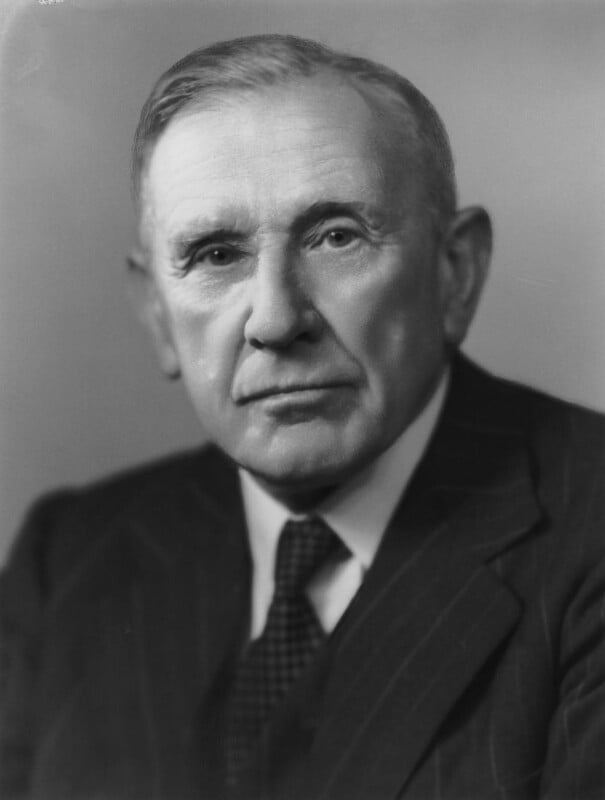
\includegraphics[height=0.38\textheight]{ch8_hurst_1953.jpg}\\[1mm]
\imgcap{H. E. Hurst (1880--1978)}
\imgcredit{https://commons.wikimedia.org/wiki/File:Harold_Edwin_Hurst_in_1953.jpg}{Photo: Elliott \& Fry (1953); public domain; Wikimedia Commons}
\end{column}
\begin{column}{0.6\textwidth}
\begin{itemize}
    \item Hurst spent more than 60 years in Egypt measuring the Nile, to size the reservoirs of the Aswan dams
    \begin{itemize}
        \item a reservoir must cover the longest run of dry years: its size depends on the \textbf{range} of cumulative inflows
    \end{itemize}
    \item \refHurst: the range grows like $n^{H}$ with $H \approx 0.7$, not like $n^{0.5}$ as for independent years
    \begin{itemize}
        \item wet years cluster with wet years and dry with dry, over decades: the ``Joseph effect'' of \refNoah
    \end{itemize}
    \item This is \textbf{long memory}: a dependence that fades too slowly for any low-order ARMA model
\end{itemize}\centering
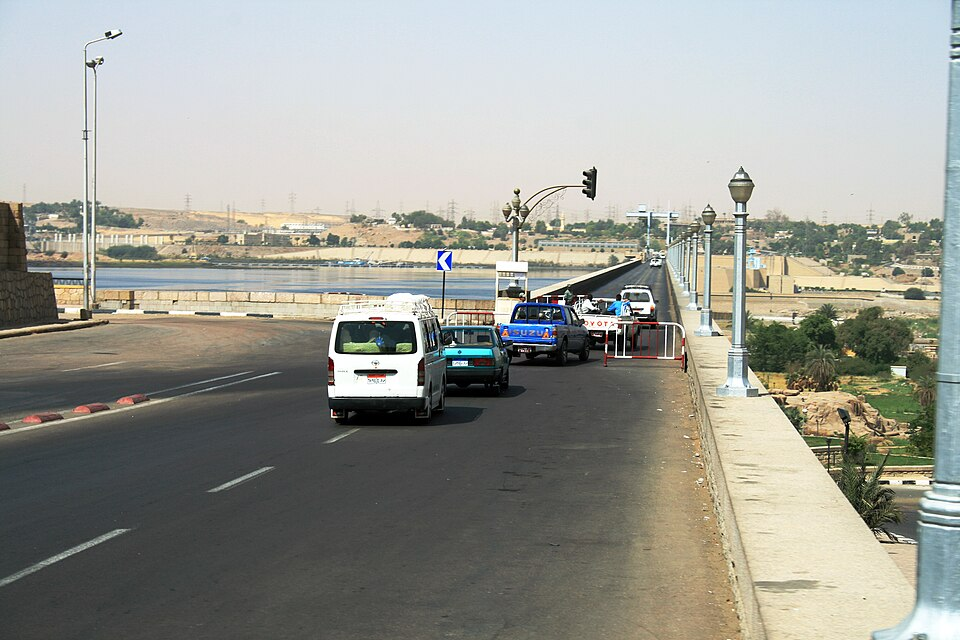
\includegraphics[height=0.17\textheight]{ch8_aswan_low_dam.jpg}\\[1mm]
\imgcap{The Aswan Low Dam (1902), on the Nile}
\imgcredit{https://commons.wikimedia.org/wiki/File:Aswan_Low_Dam_Egypt_1.jpg}{Photo: Karelj (2010); public domain; Wikimedia Commons}
\end{column}
\end{columns}
\end{frame}

\begin{frame}{Four persistent series}
\itemsize{\footnotesize}
\begin{center}
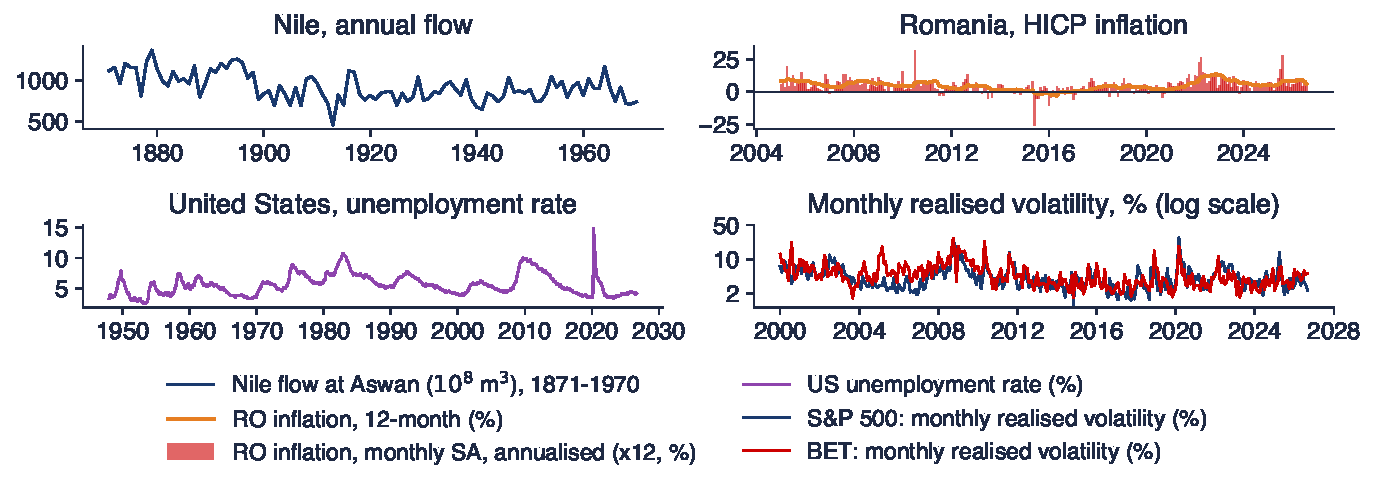
\includegraphics[width=0.97\textwidth,height=0.66\textheight,keepaspectratio]{tsa_ch8_memory_data.pdf}
\end{center}
\vspace{-0.25cm}
\begin{itemize}
    \item Nile flow at Aswan, 1871--1970 (statsmodels); Romanian HICP inflation, 12-month and monthly, seasonally adjusted (SA) with the monthly means (Eurostat)
    \item US unemployment rate (FRED UNRATE); monthly realised volatility of daily S\&P 500 and BET returns (EODHD)
\end{itemize}
\quantlet{TSA\_ch8\_memory\_data}{\qlurl{TSA_ch8_memory_data}}
\end{frame}

\begin{frame}{Interpreting the four series}
\itemsize{\small}
\begin{itemize}
    \item Each series stays above or below its mean for long stretches
    \begin{itemize}
        \item Nile: mean 919 ($10^8$ m$^3$), long dry spells after 1900; Romanian 12-month inflation peaked at 13.6\% in November 2022 and was 6.1\% in August 2026
    \end{itemize}
    \item US unemployment rises fast in recessions (peak 14.8\% in April 2020) and falls back slowly; latest 4.2\% (September 2026)
    \begin{itemize}
        \item realised volatility: calm and turbulent years alternate; maxima 27\% (S\&P 500, March 2020) and 27\% (BET, October 2008)
    \end{itemize}
    \item The question of the chapter: is this a slowly decaying (long) memory, a near unit root, or a sequence of regimes?
\end{itemize}
\end{frame}

\begin{frame}{Short memory}
\itemsize{\small}
\begin{itemize}
    \item Recall (\tsachlink{https://danpele.github.io/Time-Series-Analysis/EN/Courses/chapter1_stochastic_processes_stationarity.pdf}{Chapter 1}): $\rho(k) = \gamma(k)/\gamma(0)$, the autocorrelation at lag $k$ of a stationary series
    \begin{itemize}
        \item \textbf{short memory}: the autocorrelations are absolutely summable, $\sum_{k=0}^{\infty}|\rho(k)| < \infty$
    \end{itemize}
    \item Stationary ARMA processes: $|\rho(k)| \le C r^k$ with $0 < r < 1$: \textbf{exponential} decay
    \begin{itemize}
        \item $C > 0$: a constant; $r$: the decay rate per lag (for an AR(1), $r = |\phi|$)
        \item AR(1): $\rho(k) = \phi^k$; with $\phi = 0.9$, $\rho(50) = 0.005$: after 50 periods the shock is forgotten
    \end{itemize}
    \item Spectral view: the spectral density $f(\lambda)$ is finite and positive at frequency $\lambda = 0$
    \begin{itemize}
        \item $\lambda \in [0, \pi]$: the frequency in radians per period (a cycle of length $2\pi/\lambda$ periods)
        \item $\gamma(k)$: the autocovariance at lag $k$
        \item $f(0) = \frac{1}{2\pi}\sum_k \gamma(k)$: the long-run variance is finite; the variance of the sample mean falls like $1/T$
    \end{itemize}
\end{itemize}
\end{frame}

\begin{frame}{Long memory}
\itemsize{\small}
\begin{itemize}
    \item \textbf{Long memory} (long-range dependence): $\rho(k) \sim C\,k^{2d-1}$ as $k \to \infty$, with $0 < d < 1/2$
    \begin{itemize}
        \item a \textbf{hyperbolic} (power-law) decay: the exponent $2d - 1$ lies in $(-1, 0)$
        \item the sum $\sum_k \rho(k)$ diverges: distant observations still matter together
        \item $\sim$: the ratio of the two sides tends to 1; $C, G, c > 0$: constants; $d$: the memory parameter
    \end{itemize}
    \item Spectral view: $f(\lambda) \sim G\,\lambda^{-2d}$ as $\lambda \to 0$: a \textbf{pole} at frequency zero
    \begin{itemize}
        \item the low frequencies (slow cycles of all lengths) carry most of the variance
    \end{itemize}
    \item Consequence: $\Var(\bar{x}_T) \sim c\,T^{2d-1}$ ($\bar{x}_T$: the sample mean of $T$ observations), slower than $1/T$
    \begin{itemize}
        \item confidence intervals that assume independence are too narrow; the memory parameter $d$ measures how slowly the past fades
    \end{itemize}
\end{itemize}
\end{frame}

\begin{frame}{Sample ACF against an AR(1)}
\itemsize{\footnotesize}
\begin{center}
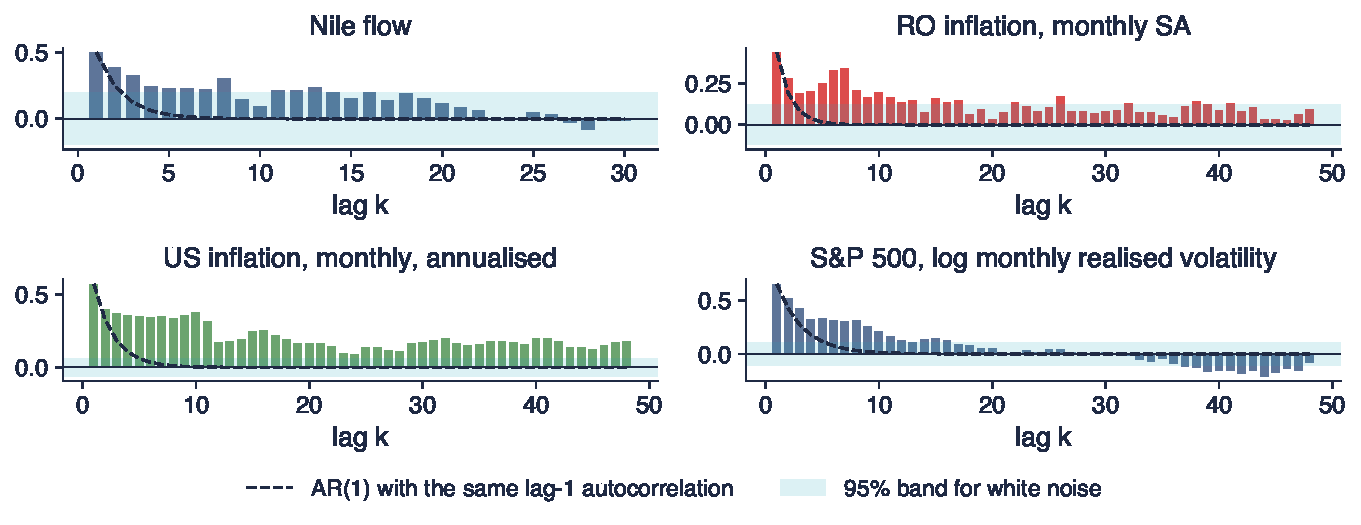
\includegraphics[width=0.97\textwidth,height=0.7\textheight,keepaspectratio]{tsa_ch8_memory_acf.pdf}
\end{center}
\vspace{-0.25cm}
\begin{itemize}
    \item Bars: sample ACF; dashed line: $\hat\rho(1)^k$, the ACF of an AR(1) with the same lag-1 autocorrelation; shaded: $\pm 1.96/\sqrt{T}$
\end{itemize}
\quantlet{TSA\_ch8\_memory\_data}{\qlurl{TSA_ch8_memory_data}}
\end{frame}

\begin{frame}{Interpreting the sample ACF}
\itemsize{\small}
\begin{itemize}
    \item Nile: $\hat\rho(1) = 0.50$; an AR(1) would give $\rho(10) = 0.0009$, the data give 0.09
    \begin{itemize}
        \item 11 of the first 30 autocorrelations lie above the white-noise band
    \end{itemize}
    \item Romanian monthly inflation: $\hat\rho(1) = 0.44$, $\hat\rho(10) = 0.20$; 22 of 48 lags above the band
    \begin{itemize}
        \item US monthly inflation: 48 of 48; S\&P 500 log realised volatility: 15 of 48
    \end{itemize}
    \item A low first autocorrelation with a long, slowly decaying tail is the signature of long memory; an AR(1) cannot produce it
\end{itemize}
\end{frame}

\begin{frame}{Hyperbolic against exponential decay}
\itemsize{\footnotesize}
\begin{center}
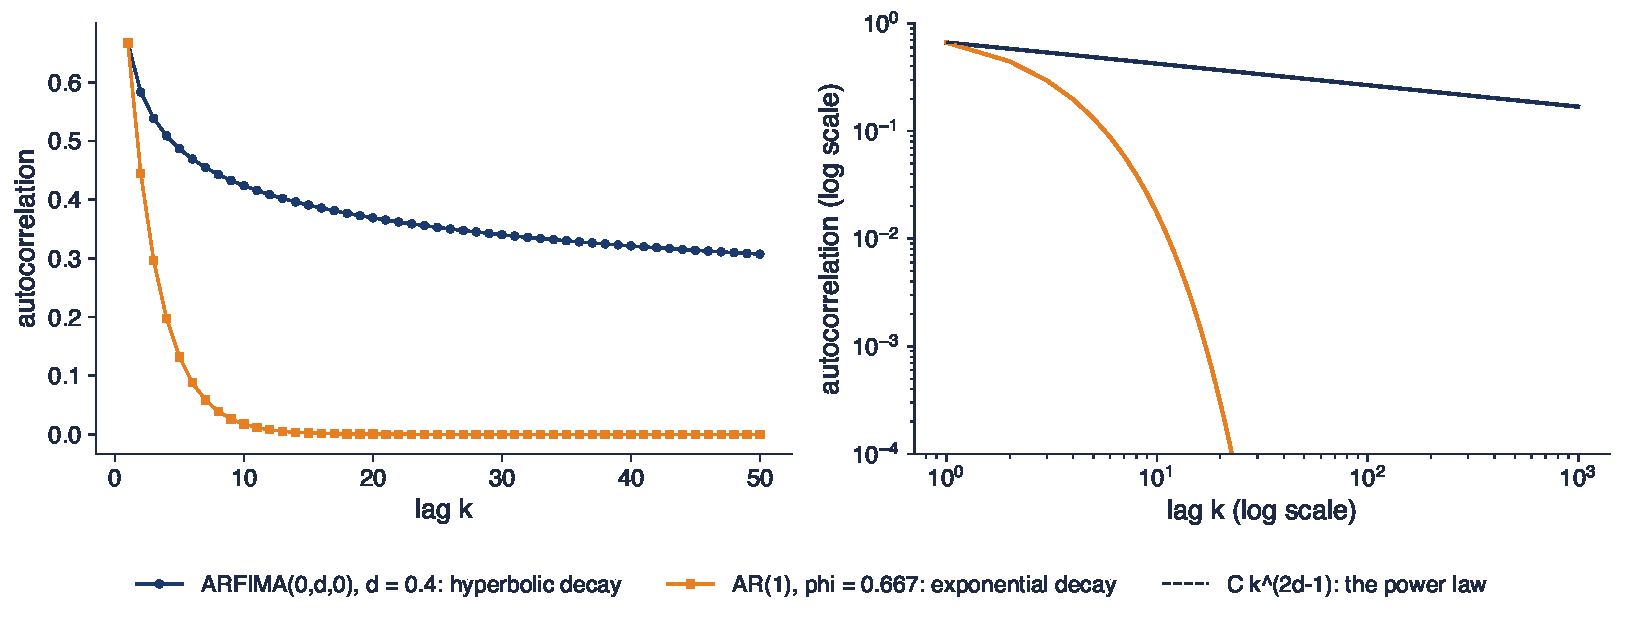
\includegraphics[width=0.97\textwidth,height=0.7\textheight,keepaspectratio]{tsa_ch8_decay.pdf}
\end{center}
\vspace{-0.25cm}
\begin{itemize}
    \item Theoretical ACF of ARFIMA$(0,d,0)$ with $d = 0.4$ (next sections) and of an AR(1) with the same $\rho(1) = d/(1-d) = 0.667$; right: both on log--log axes, with the power law $C k^{2d-1}$
\end{itemize}
\quantlet{TSA\_ch8\_arfima\_processes}{\qlurl{TSA_ch8_arfima_processes}}
\end{frame}

\begin{frame}{Interpreting the two decay laws}
\itemsize{\small}
\begin{itemize}
    \item Same start, different tails: at lag 10, 0.424 against 0.017; at lag 50, 0.307 against $1.6 \cdot 10^{-9}$
    \begin{itemize}
        \item the long-memory ACF is still 0.169 at lag 1000
    \end{itemize}
    \item On log--log axes the hyperbolic ACF becomes a straight line of slope $2d - 1 = -0.2$; the exponential ACF bends down
    \begin{itemize}
        \item the slope of a log--log plot is the idea behind every estimator of this chapter
    \end{itemize}
    \item Sums of autocorrelations: AR(1) $\sum_{k\ge1}\phi^k = 2.0$; ARFIMA: 33.0 up to lag 100 and 210.4 up to lag 1000, still growing
\end{itemize}
\end{frame}

\begin{frame}{Recap: Short and long memory}
\itemsize{\small}
\begin{itemize}
    \item Short memory: summable ACF, exponential decay, finite spectrum at zero (ARMA)
    \item Long memory: $\rho(k) \sim Ck^{2d-1}$, non-summable ACF, spectral pole $f(\lambda) \sim G\lambda^{-2d}$
    \item Hurst and the Nile: ranges grow like $n^H$, $H > 1/2$
    \item Inflation and volatility show long, slowly decaying ACF tails
\end{itemize}
\end{frame}


%=============================================================================
\section{Fractional differencing}
%=============================================================================

\begin{frame}{From integer to fractional differences}
\itemsize{\small}
\begin{itemize}
    \item Lag operator: $Lx_t = x_{t-1}$; first difference $(1-L)x_t = x_t - x_{t-1}$ (\tsachlink{https://danpele.github.io/Time-Series-Analysis/EN/Courses/chapter3_unit_roots_arima_models.pdf}{Chapter 3})
    \begin{itemize}
        \item $d = 0$: the level; $d = 1$: the first difference; $d = 2$: $x_t - 2x_{t-1} + x_{t-2}$
    \end{itemize}
    \item \textbf{Fractional difference} for any real $d$ (binomial series)
    \begin{itemize}
        \item $(1-L)^d = \sum_{k=0}^{\infty}\binom{d}{k}(-L)^k = \sum_{k=0}^{\infty}\pi_k L^k$
        \item $(1-L)^d = 1 - dL - \frac{d(1-d)}{2!}L^2 - \frac{d(1-d)(2-d)}{3!}L^3 - \dots$
        \item recursion: $\pi_0 = 1$, $\pi_k = \pi_{k-1}\,\dfrac{k - 1 - d}{k}$; for large $k$: $\pi_k \approx -\dfrac{d}{\Gamma(1-d)}\,k^{-1-d}$
        \item $\binom{d}{k} = d(d-1)\cdots(d-k+1)/k!$: the binomial coefficient for real $d$; $\pi_k$: the weight of $x_{t-k}$; $\Gamma(\cdot)$: the gamma function, $\Gamma(n) = (n-1)!$ for integers
    \end{itemize}
    \item A fractional difference uses \textbf{all} past values, with weights that decay hyperbolically: it removes part of the memory, not all of it
\end{itemize}
\end{frame}

\begin{frame}{Worked example: the weights of $(1-L)^{0.4}$}
\itemsize{\small}
\begin{itemize}
    \item Recursion $\pi_k = \pi_{k-1}(k - 1 - d)/k$ with $d = 0.4$:
    \begin{itemize}
        \item $\pi_1 = 1 \cdot (0 - 0.4)/1 = -0.40$
        \item $\pi_2 = -0.40 \cdot (1 - 0.4)/2 = -0.12$
        \item $\pi_3 = -0.12 \cdot (2 - 0.4)/3 = -0.0640$; \quad $\pi_4 = -0.0640 \cdot 3.6/4 = -0.0416$; \quad $\pi_5 = -0.0300$
    \end{itemize}
    \item So $(1-L)^{0.4}x_t = x_t - 0.4x_{t-1} - 0.12x_{t-2} - 0.064x_{t-3} - 0.0416x_{t-4} - \dots$
    \begin{itemize}
        \item the weights sum to $(1-1)^{0.4} = 0$ over all lags: a constant level is removed, as with $d = 1$
    \end{itemize}
    \item Compare $d = 1$: $\pi_1 = -1$ and all other weights are 0; $d = 0.7$: $\pi_1 = -0.70$, $\pi_2 = -0.105$
\end{itemize}
\end{frame}

\begin{frame}{Fractional differencing and fractional integration}
\itemsize{\footnotesize}
\begin{center}
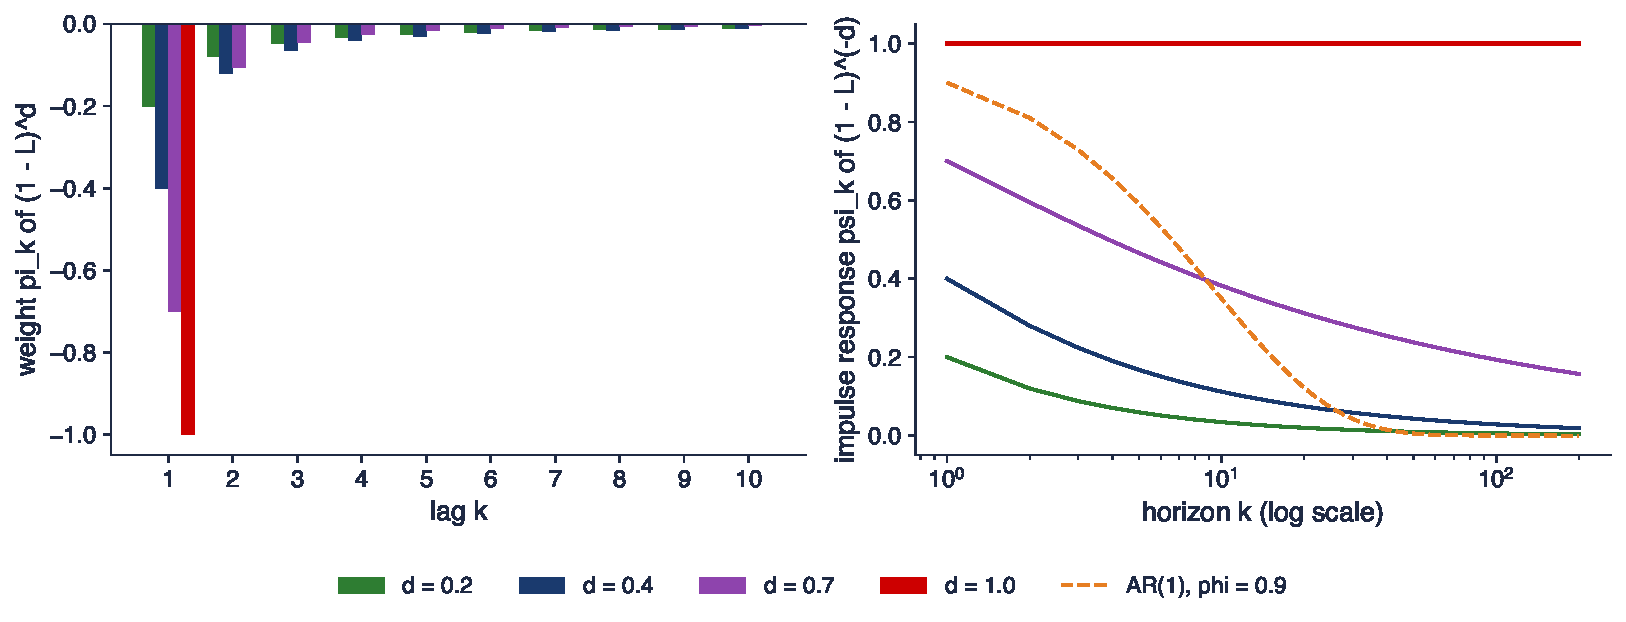
\includegraphics[width=0.97\textwidth,height=0.7\textheight,keepaspectratio]{tsa_ch8_weights.pdf}
\end{center}
\vspace{-0.25cm}
\begin{itemize}
    \item Left: weights $\pi_k$ of $(1-L)^d$; right: the impulse responses $\psi_k$ of $(1-L)^{-d}$, i.e.\ the effect after $k$ periods of a unit shock to a fractionally integrated series, against an AR(1) with $\phi = 0.9$
\end{itemize}
\quantlet{TSA\_ch8\_fractional\_differencing}{\qlurl{TSA_ch8_fractional_differencing}}
\end{frame}

\begin{frame}{Interpreting the weights}
\itemsize{\small}
\begin{itemize}
    \item Fractional integration: $x_t = (1-L)^{-d}\varepsilon_t = \sum_k\psi_k\varepsilon_{t-k}$, with $\psi_k = \psi_{k-1}(k-1+d)/k \approx k^{d-1}/\Gamma(d)$
    \begin{itemize}
        \item after 100 periods a shock still has weight 0.028 ($d = 0.4$) and 0.193 ($d = 0.7$); the AR(1) keeps $2.7 \cdot 10^{-5}$
    \end{itemize}
    \item Early on the AR(1) remembers more (0.349 at lag 10, against 0.112 for $d = 0.4$); later it forgets much faster
    \begin{itemize}
        \item $d = 1$ (random walk): $\psi_k = 1$ forever, the shock never fades
    \end{itemize}
    \item For $0 < d < 1$ the responses tend to zero: the series is \textbf{mean-reverting}, even when it is non-stationary ($d \ge 0.5$)
\end{itemize}
\end{frame}

\begin{frame}{The degree of differencing a price needs}
\itemsize{\footnotesize}
\begin{center}
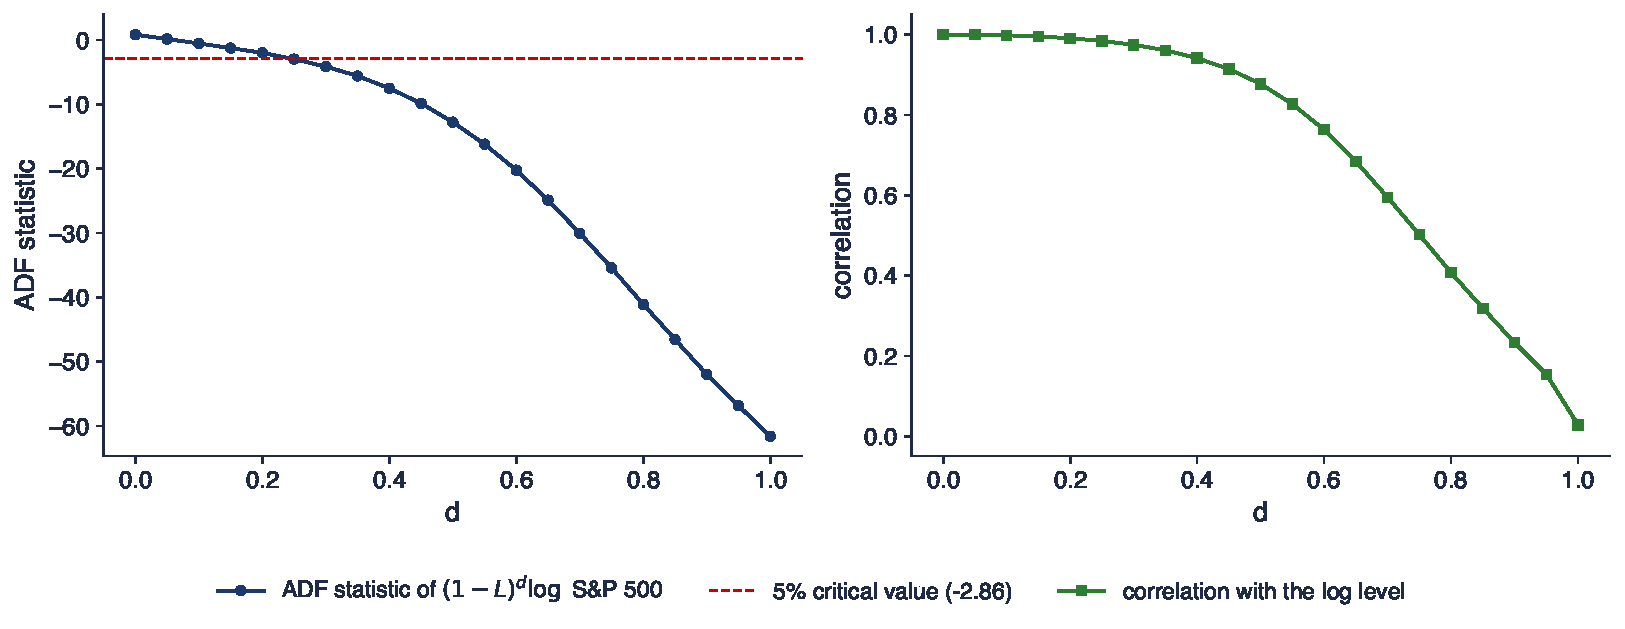
\includegraphics[width=0.97\textwidth,height=0.7\textheight,keepaspectratio]{tsa_ch8_ffd.pdf}
\end{center}
\vspace{-0.25cm}
\begin{itemize}
    \item Log S\&P 500, daily, 6\,715 days since 2000; $(1-L)^d$ with a fixed window (weights below $10^{-4}$ dropped), $d = 0, 0.05, \dots, 1$; left: ADF statistic (\tsachlink{https://danpele.github.io/Time-Series-Analysis/EN/Courses/chapter3_unit_roots_arima_models.pdf}{Chapter 3}); right: correlation with the log level
\end{itemize}
\quantlet{TSA\_ch8\_fractional\_differencing}{\qlurl{TSA_ch8_fractional_differencing}}
\end{frame}

\begin{frame}{Interpreting fractional differencing of a price}
\itemsize{\small}
\begin{itemize}
    \item The log level ($d = 0$) has a unit root (ADF 0.84); the return ($d = 1$) is stationary (ADF $-$61.6) but has correlation 0.03 with the level
    \begin{itemize}
        \item the first difference throws away all the information about the level
    \end{itemize}
    \item The ADF statistic crosses the 5\% critical value ($-$2.86) already at $d = 0.25$, where the correlation with the level is still 0.984
    \begin{itemize}
        \item the fixed window then has 445 weights
    \end{itemize}
    \item A fractional difference can make a series stationary while keeping most of its memory: a tool used for forecasting features in machine learning (\tsachlink{https://danpele.github.io/Time-Series-Analysis/EN/Courses/chapter9_machine_learning_time_series.pdf}{Chapter 9})
\end{itemize}
\end{frame}

\begin{frame}{Recap: Fractional differencing}
\itemsize{\small}
\begin{itemize}
    \item $(1-L)^d = \sum_k\pi_k L^k$, $\pi_k = \pi_{k-1}(k-1-d)/k$: hyperbolically decaying weights
    \item $(1-L)^{-d}$: impulse responses $\psi_k \approx k^{d-1}/\Gamma(d)$; mean reversion for $d < 1$
    \item $d$ between 0 and 1 fills the gap between levels and first differences
\end{itemize}
\end{frame}


%=============================================================================
\section{The ARFIMA$(p,d,q)$ model}
%=============================================================================

\begin{frame}{The ARFIMA$(p,d,q)$ model}
\itemsize{\small}
\begin{itemize}
    \item \textbf{Definition}: $\phi(L)(1-L)^d(x_t - \mu) = \theta(L)\varepsilon_t$, $\varepsilon_t$ white noise with variance $\sigma^2$
    \begin{itemize}
        \item $\phi(L) = 1 - \phi_1L - \dots - \phi_pL^p$ and $\theta(L) = 1 + \theta_1L + \dots + \theta_qL^q$, with roots outside the unit circle (\tsachlink{https://danpele.github.io/Time-Series-Analysis/EN/Courses/chapter2_arma_models.pdf}{Chapter 2})
        \item $\mu$: the mean of $x_t$; ARFIMA: autoregressive fractionally integrated moving average
    \end{itemize}
    \item Two parts with two jobs
    \begin{itemize}
        \item $d$: the \textbf{long-run} memory, the hyperbolic tail of the ACF
        \item $\phi$, $\theta$: the \textbf{short-run} dynamics, the first few autocorrelations
    \end{itemize}
    \item Special cases: $d = 0$: ARMA$(p,q)$; $d = 1$: ARIMA$(p,1,q)$ (\tsachlink{https://danpele.github.io/Time-Series-Analysis/EN/Courses/chapter3_unit_roots_arima_models.pdf}{Chapter 3}); $d$ between them: fractional integration, $x_t \sim I(d)$
\end{itemize}
\end{frame}

\begin{frame}{Granger, Joyeux and Hosking (1980--1981)}
\itemsize{\small}
\begin{columns}[T]
\begin{column}{0.38\textwidth}
\centering
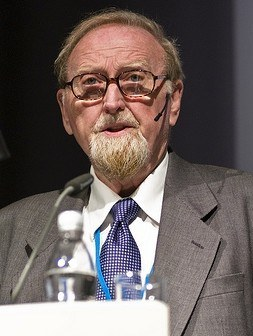
\includegraphics[height=0.48\textheight]{ch3_clive_granger_2008.jpg}\\[1mm]
\imgcap{Clive W. J. Granger (1934--2009), Nobel Prize 2003}
\imgcredit{https://commons.wikimedia.org/wiki/File:Clive_Granger_by_Olaf_Storbeck_(3x4_cropped).jpg}{Photo: Olaf Storbeck (2008); CC BY-SA 2.0; Wikimedia Commons}
\end{column}
\begin{column}{0.6\textwidth}
\begin{itemize}
    \item \refGJ\ and \refHosking\ introduced fractional differencing independently
    \begin{itemize}
        \item Granger and Joyeux: aggregating many AR(1) series with different persistence produces long memory
        \item Hosking: the ACF, the stationarity and invertibility conditions, and the ARFIMA$(p,d,q)$ family
    \end{itemize}
    \item Their model connects the Hurst exponent of hydrology with the Box--Jenkins models of econometrics
    \item Applications followed in inflation \refHW, output, interest rates and volatility \refDGE
\end{itemize}
\end{column}
\end{columns}
\end{frame}

\begin{frame}{The parameter $d$: what each range means}
\itemsize{\small}
\begin{center}
\footnotesize
\begin{tabular}{lll}
\toprule
\textbf{Range of $d$} & \textbf{Properties} & \textbf{ACF / shocks} \\
\midrule
$d \le -0.5$ & not invertible (no AR($\infty$) form) & -- \\
$-0.5 < d < 0$ & stationary, invertible, anti-persistent & negative, summable to $-1/2$ \\
$d = 0$ & ARMA, short memory & exponential decay \\
$0 < d < 0.5$ & stationary, long memory & hyperbolic, not summable \\
$0.5 \le d < 1$ & non-stationary, mean-reverting & shocks fade, slowly \\
$d = 1$ & unit root, ARIMA & shocks are permanent \\
\bottomrule
\end{tabular}
\end{center}
\begin{itemize}
    \item Stationarity needs $d < 1/2$, invertibility needs $d > -1/2$ (\refHosking); a non-stationary series with $d < 1.5$ is handled by differencing once: $(1-L)x_t \sim I(d-1)$
    \item Hurst exponent of the stationary increments: $H = d + 1/2$; $H > 1/2$ persistence, $H < 1/2$ anti-persistence
\end{itemize}
\end{frame}

\begin{frame}{Autocorrelations of ARFIMA$(0,d,0)$}
\itemsize{\small}
\begin{itemize}
    \item For $x_t = (1-L)^{-d}\varepsilon_t$, $-1/2 < d < 1/2$ (\refHosking):
    \begin{itemize}
        \item variance $\gamma(0) = \sigma^2\,\dfrac{\Gamma(1-2d)}{\Gamma(1-d)^2}$
        \item autocorrelations $\rho(k) = \dfrac{\Gamma(1-d)\,\Gamma(k+d)}{\Gamma(d)\,\Gamma(k+1-d)}$, computed with $\rho(k) = \rho(k-1)\,\dfrac{k-1+d}{k-d}$
    \end{itemize}
    \item First lags: $\rho(1) = \dfrac{d}{1-d}$, \quad $\rho(2) = \dfrac{d(1+d)}{(1-d)(2-d)}$
    \begin{itemize}
        \item large $k$: $\rho(k) \approx \dfrac{\Gamma(1-d)}{\Gamma(d)}\,k^{2d-1}$, the power law of Section 1 with $C = \Gamma(1-d)/\Gamma(d)$
    \end{itemize}
    \item Spectral density ($i$: the imaginary unit): $f(\lambda) = \dfrac{\sigma^2}{2\pi}\,|1 - e^{-i\lambda}|^{-2d} = \dfrac{\sigma^2}{2\pi}\,\bigl(2\sin(\lambda/2)\bigr)^{-2d} \approx \dfrac{\sigma^2}{2\pi}\lambda^{-2d}$ near 0
\end{itemize}
\end{frame}

\begin{frame}{Worked example: ARFIMA$(0, 0.3, 0)$}
\itemsize{\small}
\begin{itemize}
    \item $\rho(1) = 0.3/0.7 = 0.429$; \quad $\rho(2) = 0.429 \cdot 1.3/1.7 = 0.328$; \quad $\rho(3) = 0.328 \cdot 2.3/2.7 = 0.279$
    \begin{itemize}
        \item continuing the recursion: $\rho(5) = 0.228$, $\rho(10) = 0.173$
    \end{itemize}
    \item Variance with $\sigma^2 = 1$: $\Gamma(0.4)/\Gamma(0.7)^2 = 1.316$, larger than the variance of the shocks
    \begin{itemize}
        \item the memory accumulates past shocks
    \end{itemize}
    \item An AR(1) with the same $\rho(1) = 0.429$ has $\rho(10) = 0.429^{10} = 0.0002$: three orders of magnitude below 0.173
    \item $H = d + 0.5 = 0.8$: a persistent series
\end{itemize}
\end{frame}

\begin{frame}{ARFIMA$(0,d,0)$ with $d = 0.4$ and $d = -0.4$}
\itemsize{\footnotesize}
\begin{center}
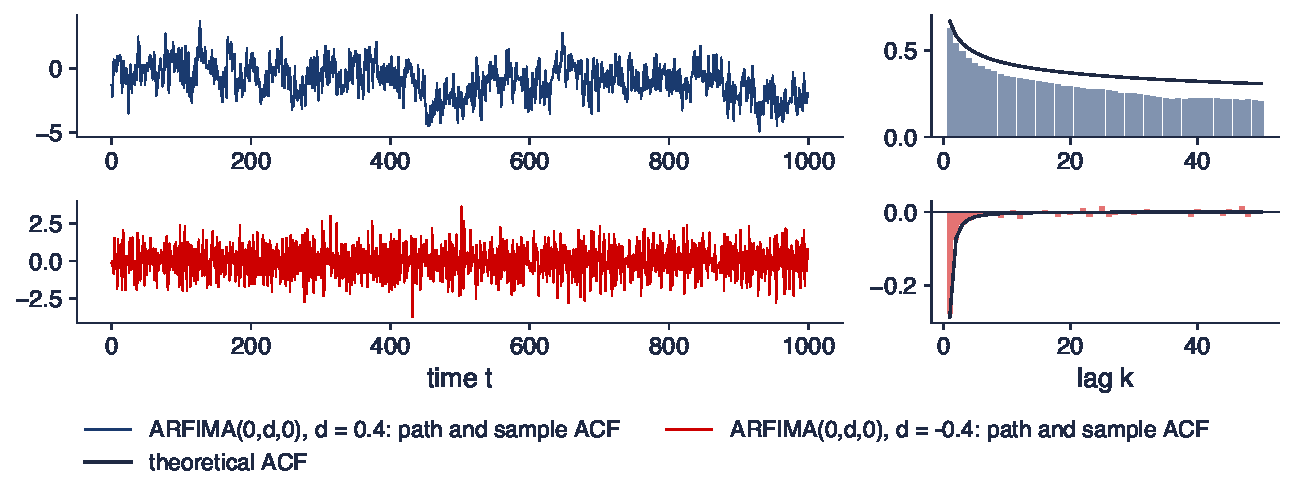
\includegraphics[width=0.97\textwidth,height=0.7\textheight,keepaspectratio]{tsa_ch8_arfima_paths.pdf}
\end{center}
\vspace{-0.25cm}
\begin{itemize}
    \item Simulated paths (1000 observations, exact simulation by circulant embedding) with $\varepsilon_t \sim N(0, 1)$; right: sample ACF of 20\,000 observations and the theoretical ACF
\end{itemize}
\quantlet{TSA\_ch8\_arfima\_processes}{\qlurl{TSA_ch8_arfima_processes}}
\end{frame}

\begin{frame}{Interpreting the two ARFIMA paths}
\itemsize{\small}
\begin{itemize}
    \item $d = 0.4$: long excursions above and below zero; $\rho(1) = 0.667$, $\rho(10) = 0.424$, $\rho(50) = 0.307$; variance 2.07
    \begin{itemize}
        \item the path looks as if it had trends, although the mean is constant: a reason why long memory is mistaken for non-stationarity
    \end{itemize}
    \item $d = -0.4$: rapid zig-zag; $\rho(1) = -0.286$, $\rho(2) = -0.071$; variance 1.18
    \begin{itemize}
        \item anti-persistence: a rise tends to be followed by a fall; typical of over-differenced series, e.g.\ the difference of a series with $d = 0.6$
    \end{itemize}
\end{itemize}
\end{frame}

\begin{frame}{Mandelbrot: fractional Brownian motion and $H$}
\itemsize{\small}
\begin{columns}[T]
\begin{column}{0.38\textwidth}
\centering
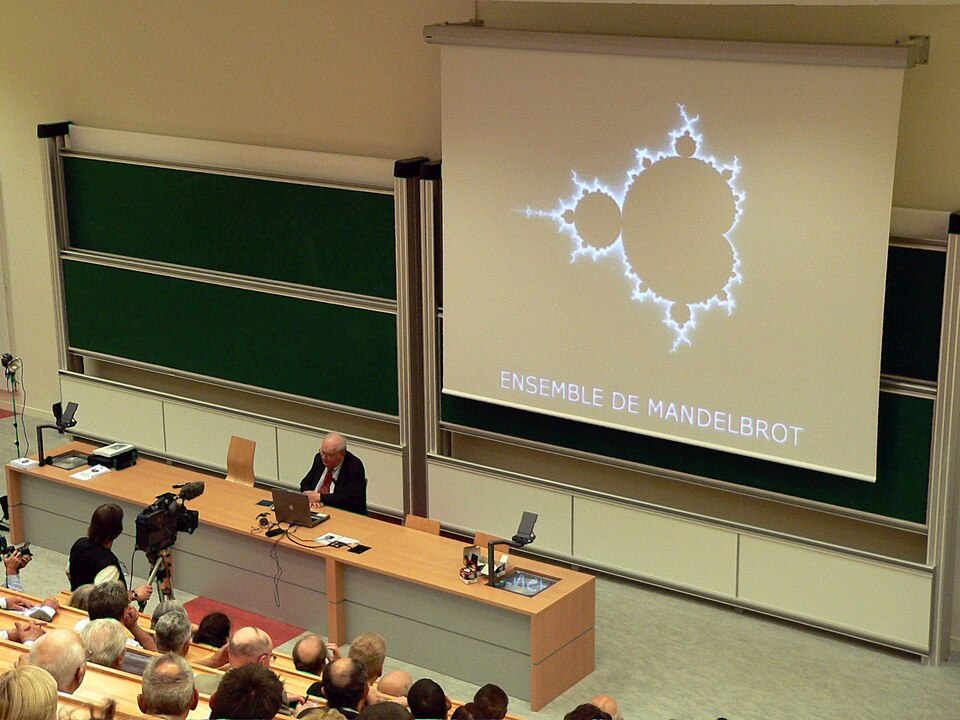
\includegraphics[height=0.42\textheight]{ch8_mandelbrot_2006.jpg}\\[1mm]
\imgcap{Benoît Mandelbrot (1924--2010)}
\imgcredit{https://commons.wikimedia.org/wiki/File:Mandelbrot_p1130876.jpg}{Photo: David Monniaux (2006); CC BY-SA 3.0; Wikimedia Commons}
\end{column}
\begin{column}{0.6\textwidth}
\begin{itemize}
    \item \textbf{Fractional Brownian motion} $B_H(t)$, $0 < H < 1$ \refMVN: Gaussian, $B_H(0) = 0$, $\Var(B_H(t)) = t^{2H}$
    \begin{itemize}
        \item self-similar: $B_H(ct)$ has the same distribution as $c^H B_H(t)$; $H = 1/2$: Brownian motion
    \end{itemize}
    \item Its increments, \textbf{fractional Gaussian noise} (fGn), are stationary with $\rho(k) = \tfrac12(|k+1|^{2H} - 2|k|^{2H} + |k-1|^{2H})$
    \begin{itemize}
        \item $\rho(k) \approx H(2H-1)k^{2H-2}$: the same tail as ARFIMA with $d = H - 1/2$
    \end{itemize}
    \item Mandelbrot brought Hurst's finding into statistics: fGn is the continuous-time cousin of ARFIMA$(0,d,0)$
\end{itemize}
\end{column}
\end{columns}
\end{frame}

\begin{frame}{Fractional Brownian motion for three Hurst exponents}
\itemsize{\footnotesize}
\begin{center}
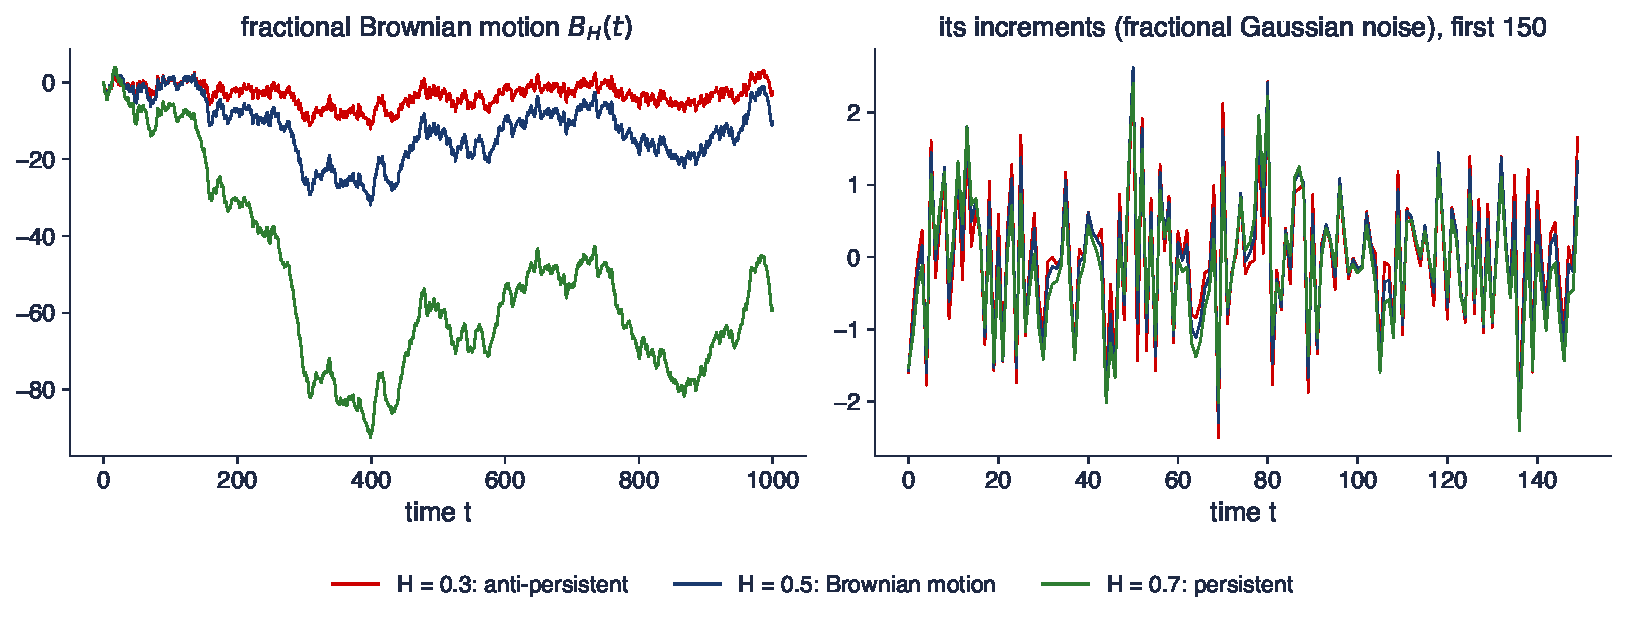
\includegraphics[width=0.97\textwidth,height=0.7\textheight,keepaspectratio]{tsa_ch8_fbm.pdf}
\end{center}
\vspace{-0.25cm}
\begin{itemize}
    \item The same random numbers for $H = 0.3$, $0.5$ and $0.7$ (circulant embedding); right: the first 150 increments
\end{itemize}
\quantlet{TSA\_ch8\_arfima\_processes}{\qlurl{TSA_ch8_arfima_processes}}
\end{frame}

\begin{frame}{Interpreting the fBm paths}
\itemsize{\small}
\begin{itemize}
    \item $H = 0.7$: smooth, trending path; lag-1 autocorrelation of the increments $2^{2H-1} - 1 = 0.32$ (sample 0.32)
    \begin{itemize}
        \item $H = 0.3$: rough path that keeps turning back; $\rho(1) = -0.24$ (sample $-$0.23)
    \end{itemize}
    \item The range of the path grows like $t^H$: the quantity Hurst measured on the Nile
    \item In time-series modelling we prefer ARFIMA: it adds the short-run ARMA part that fGn lacks
\end{itemize}
\end{frame}

\begin{frame}{Recap: The ARFIMA model}
\itemsize{\small}
\begin{itemize}
    \item $\phi(L)(1-L)^d(x_t - \mu) = \theta(L)\varepsilon_t$: $d$ for the long run, ARMA for the short run
    \item Stationary for $d < 1/2$, invertible for $d > -1/2$; mean-reverting for $d < 1$
    \item ARFIMA$(0,d,0)$: $\rho(1) = d/(1-d)$, $\rho(k) \sim Ck^{2d-1}$; $H = d + 1/2$
    \item fBm and fGn: the same long memory in Mandelbrot's continuous-time form
\end{itemize}
\end{frame}


%=============================================================================
\section{Estimating $d$}
%=============================================================================

\begin{frame}{Five estimators}
\itemsize{\small}
\begin{center}
\scriptsize
\begin{tabular}{>{\raggedright\arraybackslash}p{2.3cm}>{\raggedright\arraybackslash}p{3.1cm}>{\raggedright\arraybackslash}p{3.6cm}>{\raggedright\arraybackslash}p{1.9cm}}
\toprule
\textbf{Estimator} & \textbf{Uses} & \textbf{Estimate} & \textbf{Type} \\
\midrule
R/S \refHurst{} & range of partial sums in blocks & slope of $\log(R/S)_n$ on $\log n$ = $H$ & heuristic \\
DFA \refPeng{} & detrended fluctuations of the profile & slope of $\log F(n)$ on $\log n$ = $H$ & heuristic \\
GPH \refGPH{} & lowest $m$ periodogram ordinates & OLS slope of a log-periodogram regression & semiparametric \\
Local Whittle \refRob{} & lowest $m$ periodogram ordinates & maximises a local Gaussian likelihood & semiparametric \\
Exact ML, Whittle \refSowell, \refFT{} & the whole series & $d$, $\phi$, $\theta$, $\sigma^2$ jointly & parametric \\
\bottomrule
\end{tabular}
\end{center}
\begin{itemize}
    \item Semiparametric: only the behaviour near frequency zero is modelled, the short-run part is left free; parametric: the whole ARFIMA model must be right
    \item ML: maximum likelihood; OLS: ordinary least squares; $d = H - 1/2$ converts between the two scales
\end{itemize}
\end{frame}

\begin{frame}{The R/S statistic, step by step}
\itemsize{\footnotesize}
\begin{itemize}
    \item Block $x_1, \dots, x_n$: mean $\bar x$, cumulative deviations $Y_k = \sum_{i\le k}(x_i - \bar x)$
    \begin{itemize}
        \item range $R = \max_k Y_k - \min_k Y_k$, $S$: the standard deviation of the block; rescaled range $R/S$
    \end{itemize}
    \item Example: $x = (0.5, -0.3, 0.8, -0.2, 0.6, -0.1, 0.4, -0.7)$, $\bar x = 0.125$
    \begin{itemize}
        \item $Y_k$: 0.375, $-$0.050, 0.625, 0.300, 0.775, 0.550, 0.825, 0; $R = 0.825 - (-0.050) = 0.875$
        \item $S = 0.489$, so $R/S = 1.79$
    \end{itemize}
    \item \textbf{Hurst exponent}: average $(R/S)_n$ over blocks of size $n$; $E(R/S)_n \approx c\,n^H$, so $H$ is the slope of $\log(R/S)_n$ on $\log n$
    \begin{itemize}
        \item pitfalls: biased upwards in small blocks \refMW; short memory also raises it; \refLo\ corrects $S$ with autocovariances (modified R/S)
        \item \textbf{DFA} \refPeng: fit a line to the profile $Y_k$ in each block; $F(n)$, the RMS (root mean square) deviation, grows like $n^H$
    \end{itemize}
\end{itemize}
\end{frame}

\begin{frame}{R/S and DFA on three series}
\itemsize{\footnotesize}
\begin{center}
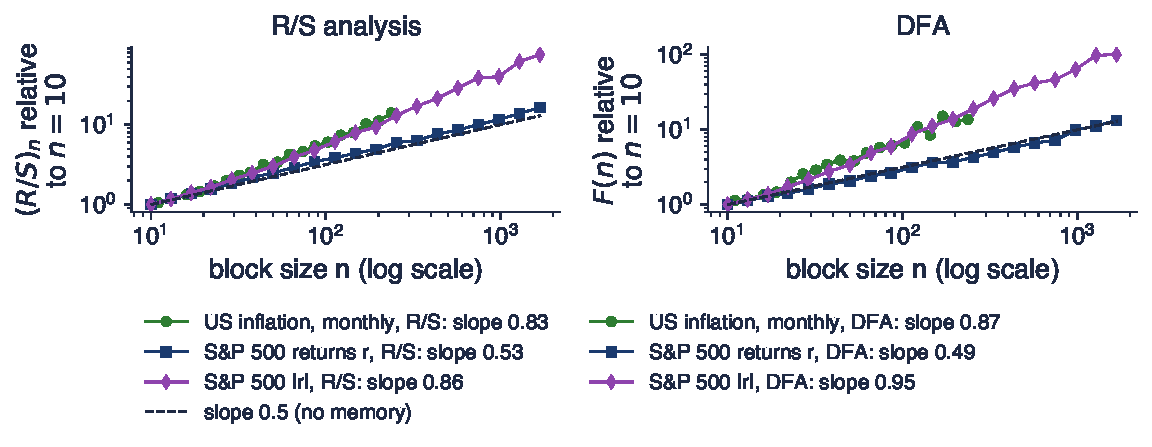
\includegraphics[width=0.97\textwidth,height=0.7\textheight,keepaspectratio]{tsa_ch8_rs_dfa.pdf}
\end{center}
\vspace{-0.25cm}
\begin{itemize}
    \item US monthly inflation (FRED CPIAUCSL, 1947--2026), daily S\&P 500 returns $r_t$ and absolute returns $|r_t|$ (2000--2026); both axes logarithmic, curves normalised to 1 at $n = 10$
\end{itemize}
\quantlet{TSA\_ch8\_hurst\_rs\_dfa}{\qlurl{TSA_ch8_hurst_rs_dfa}}
\end{frame}

\begin{frame}{Interpreting the R/S and DFA slopes}
\itemsize{\small}
\begin{itemize}
    \item S\&P 500 returns: slopes 0.53 (R/S) and 0.49 (DFA), close to 0.5: no memory in returns
    \begin{itemize}
        \item the weak efficiency of \tsachlink{https://danpele.github.io/Time-Series-Analysis/EN/Courses/chapter3_unit_roots_arima_models.pdf}{Chapter 3} holds for the level of returns
    \end{itemize}
    \item Absolute returns: 0.86 and 0.95; US inflation: 0.83 and 0.87
    \begin{itemize}
        \item both well above 0.5: persistent; a DFA slope near 1 hints at $d$ close to 0.5, the edge of stationarity
    \end{itemize}
    \item These are graphical tools: they give no standard error and react to short memory and trends; the next estimators are built for inference
\end{itemize}
\end{frame}

\begin{frame}{The periodogram and the GPH estimator}
\itemsize{\small}
\begin{itemize}
    \item \textbf{Periodogram} at the Fourier frequencies $\lambda_j = 2\pi j/T$: $I(\lambda_j) = \frac{1}{2\pi T}\bigl|\sum_t (x_t - \bar x)e^{-i\lambda_j t}\bigr|^2$
    \begin{itemize}
        \item $i$: the imaginary unit; $|\cdot|$: the modulus of a complex number; $j = 1, \dots, \lfloor T/2\rfloor$
        \item a noisy estimate of the spectral density $f(\lambda_j)$; $\lambda_j$ near 0 = slow cycles of period $T/j$
    \end{itemize}
    \item Near zero, $f(\lambda) \approx G\,(4\sin^2(\lambda/2))^{-d}$; taking logs:
    \begin{itemize}
        \item \textbf{GPH regression} \refGPH: $\log I(\lambda_j) = c + d\,\bigl[-\log(4\sin^2(\lambda_j/2))\bigr] + u_j$, $j = 1, \dots, m$
        \item $c$: constant; $u_j$: regression error; $\hat d$ = OLS slope; standard error $\pi/\sqrt{24m}$
    \end{itemize}
    \item \textbf{Bandwidth} $m$: how many low frequencies we use; here $m = \lfloor T^{0.65}\rfloor$
    \begin{itemize}
        \item small $m$: little bias from the short-run part, large variance; large $m$: small variance, but short memory leaks into $\hat d$
    \end{itemize}
\end{itemize}
\end{frame}

\begin{frame}{GPH regressions: the Nile and Romanian inflation}
\itemsize{\footnotesize}
\begin{center}
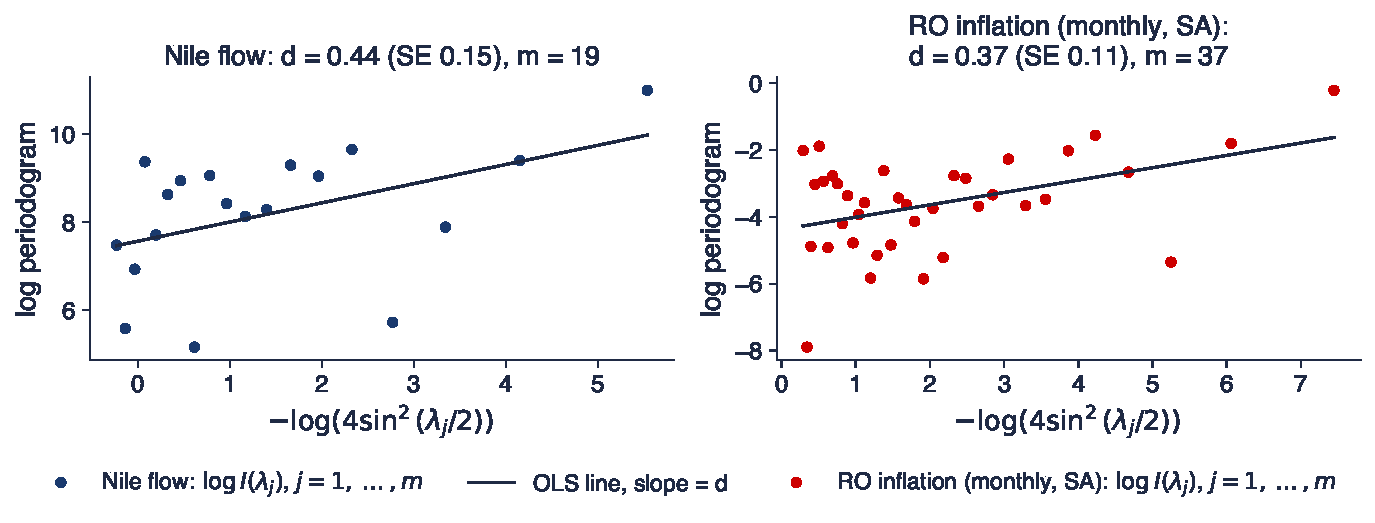
\includegraphics[width=0.97\textwidth,height=0.7\textheight,keepaspectratio]{tsa_ch8_gph.pdf}
\end{center}
\vspace{-0.25cm}
\begin{itemize}
    \item Dots: log periodogram at the $m$ lowest Fourier frequencies; line: OLS fit. Nile: $T = 100$ years; Romanian monthly inflation (SA): $T = 260$ months, August 2026 the last
\end{itemize}
\quantlet{TSA\_ch8\_estimation}{\qlurl{TSA_ch8_estimation}}
\end{frame}

\begin{frame}{Interpreting the GPH regressions}
\itemsize{\small}
\begin{itemize}
    \item Nile: $\hat d = 0.44$ (SE 0.15), $m = 19$ frequencies, i.e.\ cycles longer than 5.3 years
    \begin{itemize}
        \item local Whittle (next slide): 0.40 (SE 0.11); both significantly above 0, inside the stationary range
    \end{itemize}
    \item Romanian inflation: $\hat d = 0.37$ (SE 0.11); local Whittle 0.31 (SE 0.08)
    \begin{itemize}
        \item cycles longer than 7.0 months: a shock to monthly inflation fades over years, not months
    \end{itemize}
    \item The cloud is wide: each periodogram ordinate is roughly an exponential variable around $f(\lambda_j)$; the slope needs many points
\end{itemize}
\end{frame}

\begin{frame}{The local Whittle estimator}
\itemsize{\small}
\begin{itemize}
    \item Local Whittle (LW) \refRob
    \begin{itemize}
        \item assume $f(\lambda) \approx G\lambda^{-2d}$ for $\lambda_1, \dots, \lambda_m$ and maximise the Gaussian (Whittle) likelihood of these ordinates
        \item after concentrating out the constant $G$ of $f(\lambda) \approx G\lambda^{-2d}$: $\hat d = \arg\min_d\ \log\Bigl(\frac1m\sum_{j=1}^m \lambda_j^{2d}I(\lambda_j)\Bigr) - \frac{2d}{m}\sum_{j=1}^m\log\lambda_j$
    \end{itemize}
    \item Standard error $1/(2\sqrt m)$, smaller than GPH ($\pi/\sqrt{24m} \approx 0.64/\sqrt m$)
    \begin{itemize}
        \item valid also for non-stationary series with $d$ up to about 1 \refVelasco
    \end{itemize}
    \item Both GPH and local Whittle depend on $m$: always report $\hat d$ for several bandwidths
\end{itemize}
\end{frame}

\begin{frame}{Sensitivity to the bandwidth}
\itemsize{\footnotesize}
\begin{center}
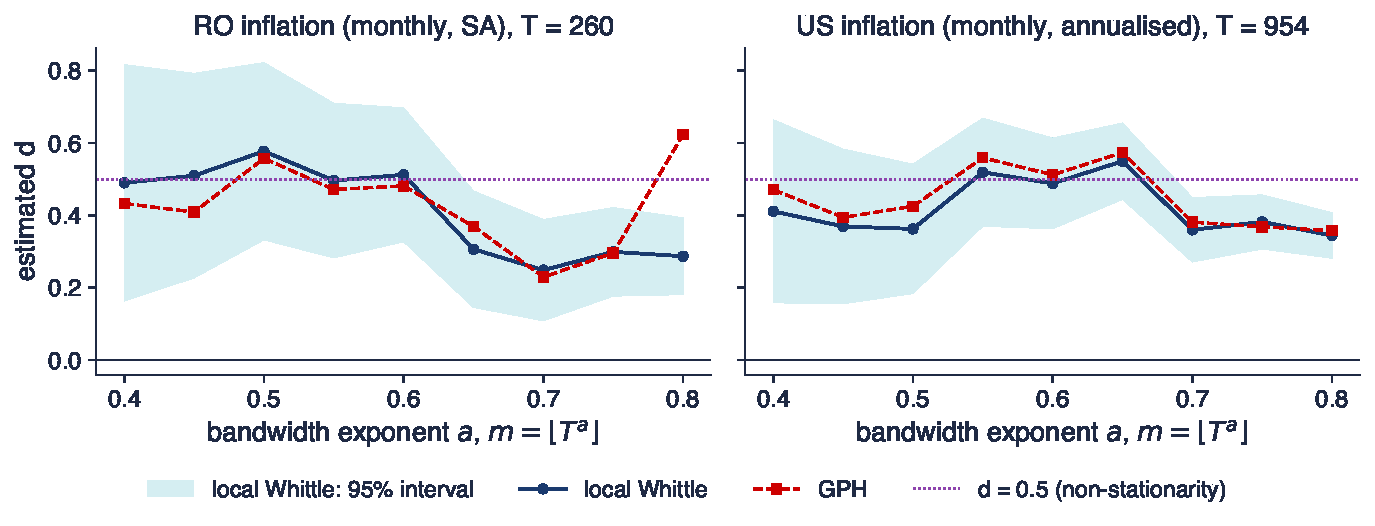
\includegraphics[width=0.97\textwidth,height=0.7\textheight,keepaspectratio]{tsa_ch8_bandwidth.pdf}
\end{center}
\vspace{-0.25cm}
\begin{itemize}
    \item $\hat d$ for $m = \lfloor T^a\rfloor$, $a = 0.40, \dots, 0.80$; shaded: 95\% interval of local Whittle. Romanian monthly inflation ($T = 260$, $m$ from 9 to 85) and US monthly inflation ($T = 954$)
\end{itemize}
\quantlet{TSA\_ch8\_estimation}{\qlurl{TSA_ch8_estimation}}
\end{frame}

\begin{frame}{Interpreting the bandwidth plot}
\itemsize{\small}
\begin{itemize}
    \item Romania: local Whittle between 0.25 and 0.58, GPH between 0.23 and 0.62
    \begin{itemize}
        \item with few frequencies the estimate is near 0.5; with more it falls to about 0.3: the answer depends on the choice of $m$
    \end{itemize}
    \item United States: local Whittle between 0.34 and 0.55, always well above 0
    \begin{itemize}
        \item the long sample (1947--2026) gives narrow intervals; the level of $d$ near 0.5 hints at regime changes (Section 7)
    \end{itemize}
    \item Conclusion: inflation has long memory in both countries; a single number for $d$ hides an uncertainty of about $\pm 0.15$
\end{itemize}
\end{frame}

\begin{frame}{Maximum likelihood for ARFIMA$(p,d,q)$}
\itemsize{\footnotesize}
\begin{itemize}
    \item \textbf{Exact ML} \refSowell: for Gaussian $x = (x_1, \dots, x_T)'$ with covariance matrix $\Gamma(\vartheta)$, $\vartheta = (d, \phi, \theta, \sigma^2)$:
    \begin{itemize}
        \item $\ell(\vartheta) = -\frac{T}{2}\log 2\pi - \frac12\log\det\Gamma(\vartheta) - \frac12 (x - \mu)'\Gamma(\vartheta)^{-1}(x - \mu)$
        \item $\ell$: the log-likelihood; $\mu$: the vector of means; $\Gamma(\vartheta)$: the $T \times T$ matrix of the ARFIMA autocovariances
        \item $\Gamma$ comes from the ARFIMA autocovariances; the Durbin--Levinson recursion evaluates $\ell$ in $O(T^2)$ operations
    \end{itemize}
    \item \textbf{Whittle} (approximate) ML \refFT: replace the likelihood by $-\frac12\sum_j\bigl[\log f(\lambda_j;\vartheta) + I(\lambda_j)/f(\lambda_j;\vartheta)\bigr]$ over all Fourier frequencies
    \begin{itemize}
        \item $f(\lambda_j;\vartheta)$: the spectral density implied by the parameters $\vartheta$
        \item fast ($O(T\log T)$ with the FFT, the fast Fourier transform), close to exact ML in large samples
    \end{itemize}
    \item Parametric estimators are efficient (SE about $\sqrt{6}/(\pi\sqrt T)$ for ARFIMA$(0,d,0)$) only if the ARMA orders are right; choose $p$, $q$ by AIC/BIC
\end{itemize}
\end{frame}

\begin{frame}{Monte Carlo: five estimators of $d$}
\itemsize{\footnotesize}
\begin{center}
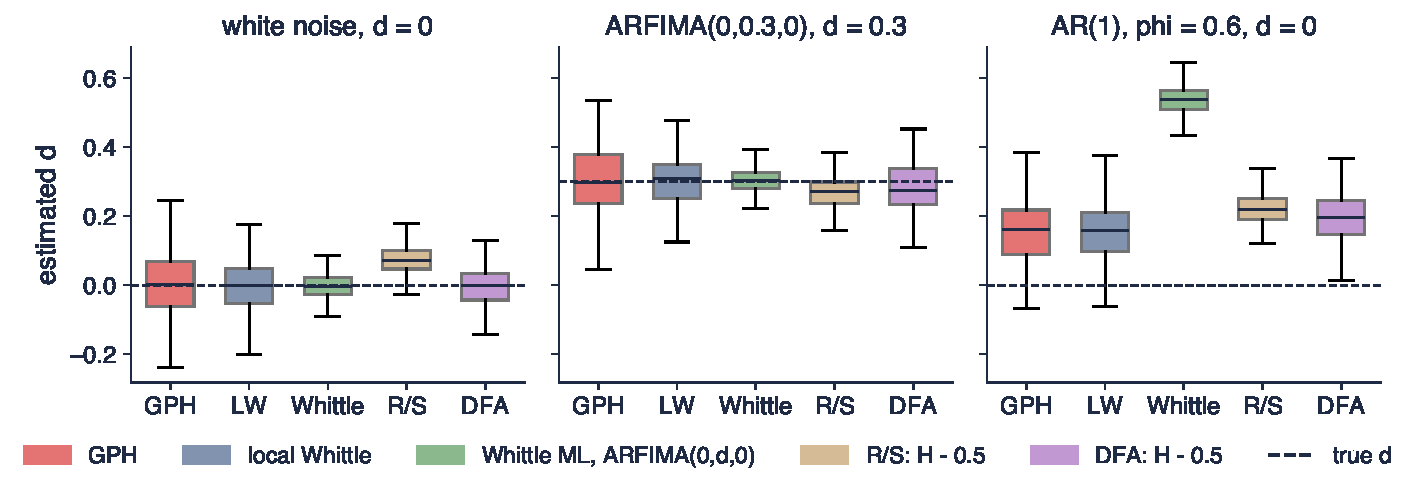
\includegraphics[width=0.97\textwidth,height=0.7\textheight,keepaspectratio]{tsa_ch8_mc.pdf}
\end{center}
\vspace{-0.25cm}
\begin{itemize}
    \item 300 samples of $T = 500$ per design; GPH and local Whittle with $m = \lfloor T^{0.65}\rfloor$; Whittle ML of ARFIMA$(0,d,0)$; R/S and DFA converted with $d = H - 1/2$
\end{itemize}
\quantlet{TSA\_ch8\_monte\_carlo}{\qlurl{TSA_ch8_monte_carlo}}
\end{frame}

\begin{frame}{Interpreting the Monte Carlo}
\itemsize{\small}
\begin{itemize}
    \item Correct model: Whittle ML is the most precise (SD 0.04 against 0.08 for local Whittle and 0.10 for GPH at $d = 0.3$)
    \begin{itemize}
        \item R/S is biased upwards under white noise (mean 0.07) \refMW
    \end{itemize}
    \item AR(1) with $\phi = 0.6$ and no long memory: ARFIMA$(0,d,0)$ by Whittle gives 0.54, GPH 0.15, local Whittle 0.15
    \begin{itemize}
        \item a misspecified parametric model turns short memory into ``long memory''; semiparametric estimators suffer less, but are not immune
    \end{itemize}
    \item Practice: always fit ARFIMA$(p,d,q)$ with $p, q \ge 1$ as alternatives, and check the semiparametric $\hat d$ for several $m$
\end{itemize}
\end{frame}

\begin{frame}{Romanian inflation: ARMA or ARFIMA?}
\itemsize{\small}
\begin{center}
\scriptsize
\begin{tabular}{lrrrrr}
\toprule
\textbf{Model (exact ML)} & $\hat d$ & \textbf{AR / MA} & $\ell$ & AIC & BIC \\
\midrule
ARMA(1,1) & 0 & 0.92 / $-$0.71 & $-$138.0 & 282.1 & 292.8 \\
ARMA(2,0) & 0 & 0.39, \dots & $-$139.9 & 285.9 & 296.6 \\
ARFIMA(0,$d$,0) & 0.31 & -- & $-$135.9 & \textbf{275.8} & \textbf{282.9} \\
ARFIMA(1,$d$,0) & 0.27 & 0.07 / -- & $-$135.6 & 277.1 & 287.8 \\
ARFIMA(0,$d$,1) & 0.27 & -- / 0.08 & $-$135.5 & 277.1 & 287.8 \\
ARFIMA(1,$d$,1) & 0.27 & $-$0.03 / 0.10 & $-$135.5 & 279.1 & 293.3 \\
\bottomrule
\end{tabular}
\end{center}
\begin{itemize}
    \item Romanian monthly HICP inflation, seasonally adjusted, $T = 260$ months (2005--2026); $\ell$: maximised log-likelihood; bold: the smallest criterion
    \item ARFIMA$(0,d,0)$ wins with one parameter: $\hat d = 0.31$ (SE 0.047); adding $\phi$ or $\theta$ barely changes $\ell$
    \item The best ARMA needs $\phi = 0.92$ close to 1 and a cancelling MA term to imitate the slow decay
\end{itemize}
\end{frame}

\begin{frame}{Romanian inflation: fitted autocorrelations}
\itemsize{\footnotesize}
\begin{center}
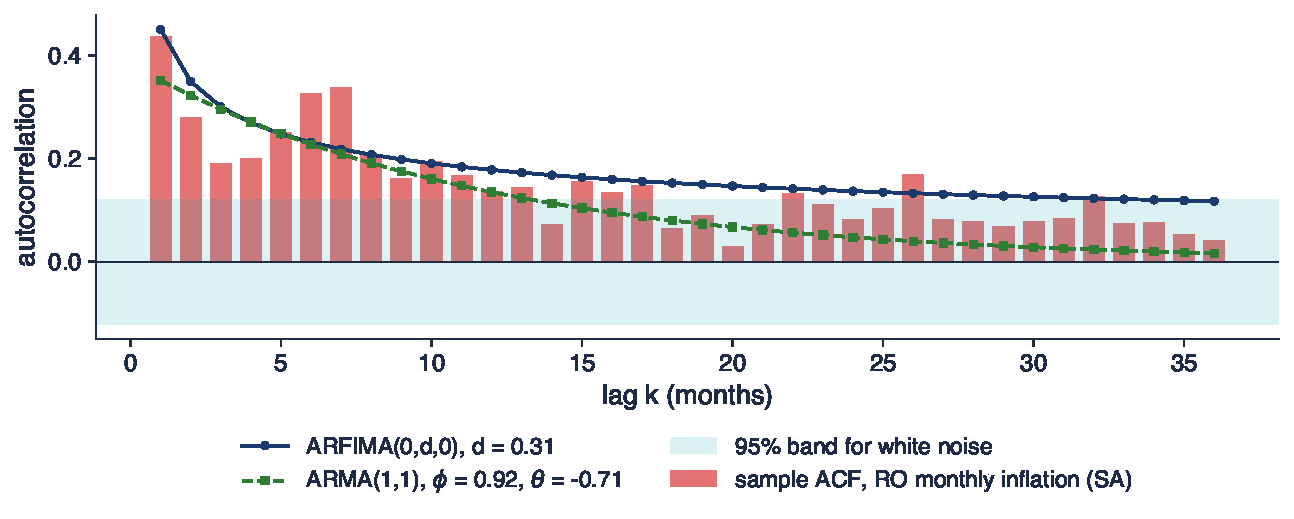
\includegraphics[width=0.97\textwidth,height=0.7\textheight,keepaspectratio]{tsa_ch8_arfima_fit.pdf}
\end{center}
\vspace{-0.25cm}
\begin{itemize}
    \item Bars: sample ACF; lines: the ACF implied by ARFIMA$(0,d,0)$ and by ARMA(1,1), both estimated by exact ML
\end{itemize}
\quantlet{TSA\_ch8\_estimation}{\qlurl{TSA_ch8_estimation}}
\end{frame}

\begin{frame}{Interpreting the fitted ACF}
\itemsize{\small}
\begin{itemize}
    \item At lag 12: sample 0.14, ARFIMA 0.18, ARMA(1,1) 0.14; at lag 24: 0.08, 0.14 and 0.05
    \begin{itemize}
        \item the two models agree on the first year and disagree on the second: their long-horizon forecasts will differ
    \end{itemize}
    \item The ARFIMA curve matches the slow tail with one parameter; the ARMA curve goes to zero exponentially
    \item Seasonal adjustment matters: a seasonal peak near the lowest frequencies would distort $\hat d$ (\tsachlink{https://danpele.github.io/Time-Series-Analysis/EN/Courses/chapter4_seasonality_forecasting.pdf}{Chapter 4})
\end{itemize}
\end{frame}

\begin{frame}{Long memory in twelve series}
\itemsize{\footnotesize}
\begin{center}
\scriptsize
\begin{tabular}{lrrrrr}
\toprule
\textbf{Series} & $T$ & $H_{R/S}$ & $H_{DFA}$ & $d_{GPH}$ & $d_{LW}$ (SE) \\
\midrule
Nile & 100 & 0.83 & 0.64 & 0.44 & 0.40 (0.11) \\
RO inflation, monthly SA & 260 & 0.75 & 0.84 & 0.37 & 0.31 (0.08) \\
RO inflation, 12-month & 260 & 0.96 & 1.38 & 1.14 & 1.00 (0.08) \\
US inflation, monthly & 954 & 0.83 & 0.87 & 0.57 & 0.55 (0.05) \\
US inflation, 1985--2019 & 420 & 0.69 & 0.59 & 0.07 & 0.10 (0.07) \\
US unemployment & 944 & 0.97 & 1.27 & 0.82 & 0.91 (0.05) \\
S\&P 500, $r_t$ & 6\,714 & 0.53 & 0.49 & 0.02 & $-$0.01 (0.03) \\
S\&P 500, $|r_t|$ & 6\,714 & 0.86 & 0.95 & 0.56 & 0.53 (0.03) \\
BET, $r_t$ & 6\,670 & 0.58 & 0.57 & 0.16 & 0.12 (0.03) \\
BET, $|r_t|$ & 6\,670 & 0.79 & 0.85 & 0.40 & 0.39 (0.03) \\
EUR/RON, $r_t$ & 5\,352 & 0.53 & 0.52 & $-$0.01 & $-$0.01 (0.03) \\
EUR/RON, $|r_t|$ & 5\,352 & 0.82 & 0.85 & 0.38 & 0.39 (0.03) \\
\bottomrule
\end{tabular}
\end{center}
\begin{itemize}
    \item $m = \lfloor T^{0.65}\rfloor$; LW: local Whittle; data: statsmodels, Eurostat, FRED, EODHD, BNR; returns daily since 2000 (EUR/RON since 2005)
\end{itemize}
\end{frame}

\begin{frame}{Interpreting the table}
\itemsize{\small}
\begin{itemize}
    \item Returns: $d \approx 0$ for the S\&P 500 ($-$0.01) and EUR/RON ($-$0.01); small but positive for the BET (0.12)
    \begin{itemize}
        \item absolute returns: 0.53, 0.39 and 0.39: long memory in volatility (Section 6)
    \end{itemize}
    \item Romanian 12-month inflation: $d \approx$ 1.00, against 0.31 for the monthly rate: the 12-month rate sums 12 overlapping monthly changes
    \begin{itemize}
        \item the overlap kills the spectrum at the frequencies used by the estimator and pushes $\hat d$ towards 1; model the monthly rate
    \end{itemize}
    \item US unemployment: $d \approx$ 0.91: non-stationary but mean-reverting; US inflation 1985--2019: 0.10, against 0.55 on 1947--2026
\end{itemize}
\end{frame}

\begin{frame}{Recap: Estimating $d$}
\itemsize{\small}
\begin{itemize}
    \item R/S and DFA: slopes of log--log plots, graphical, biased in small samples
    \item GPH and local Whittle: regressions or likelihoods on the $m$ lowest frequencies; report several $m$
    \item Exact ML and Whittle: efficient if the ARMA part is right; short memory can masquerade as $d$
    \item Romanian monthly inflation: ARFIMA$(0,d,0)$ with $\hat d = 0.31$ beats ARMA by AIC and BIC
\end{itemize}
\end{frame}


%=============================================================================
\section{Forecasting with ARFIMA}
%=============================================================================

\begin{frame}{Forecasts from the AR($\infty$) form}
\itemsize{\small}
\begin{itemize}
    \item An invertible ARFIMA can be written as $\pi(L)(x_t - \mu) = \varepsilon_t$, with $\pi(L) = \phi(L)(1-L)^d/\theta(L) = \sum_k\pi_kL^k$
    \begin{itemize}
        \item $\pi_k$: the AR($\infty$) weights (for ARFIMA$(0,d,0)$, the weights of $(1-L)^d$); $\hat x_{T+h}$: the forecast made at $T$ for $T + h$
        \item one step: $\hat x_{T+1} = \mu - \sum_{k=1}^{T}\pi_k(x_{T+1-k} - \mu)$; $h$ steps: the same recursion, with forecasts in place of unknown values
    \end{itemize}
    \item Example, ARFIMA$(0,0.4,0)$: $-\pi_k = 0.4,\ 0.12,\ 0.064,\ 0.042, \dots$
    \begin{itemize}
        \item $\hat x_{T+1} - \mu = 0.4(x_T - \mu) + 0.12(x_{T-1} - \mu) + 0.064(x_{T-2} - \mu) + \dots$: the whole history counts
        \item an AR(1) uses only $x_T$; after a long period above the mean the ARFIMA forecast stays higher, for longer
    \end{itemize}
    \item Forecasts revert to $\mu$ hyperbolically; the forecast error variance $\sigma^2\sum_{j<h}\psi_j^2$ ($\psi_j$: the MA($\infty$) weights) grows slowly towards $\gamma(0)$ \refRay
\end{itemize}
\end{frame}

\begin{frame}{US inflation: ARFIMA and AR forecasts}
\itemsize{\footnotesize}
\begin{center}
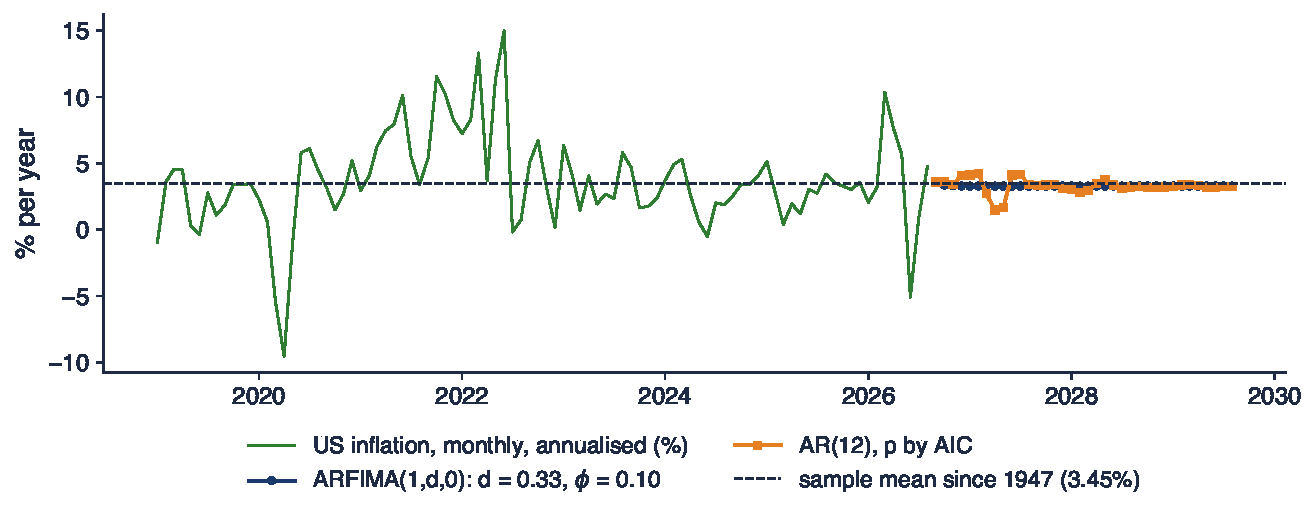
\includegraphics[width=0.97\textwidth,height=0.7\textheight,keepaspectratio]{tsa_ch8_forecast_path.pdf}
\end{center}
\vspace{-0.25cm}
\begin{itemize}
    \item US monthly CPI inflation, annualised, $T = 954$ months up to August 2026; ARFIMA(1,$d$,0) estimated by Whittle; AR($p$) with $p$ by AIC; 36 months ahead
\end{itemize}
\quantlet{TSA\_ch8\_forecasting}{\qlurl{TSA_ch8_forecasting}}
\end{frame}

\begin{frame}{Interpreting the two forecasts}
\itemsize{\small}
\begin{itemize}
    \item ARFIMA: $\hat d = 0.33$, $\hat\phi = 0.10$; AR: $p = 12$ lags, the largest allowed
    \begin{itemize}
        \item the AR needs a year of lags to imitate what $d$ does with one parameter
    \end{itemize}
    \item Last 12 months average 3.65\%; the forecasts: 3.62\% and 3.59\% next month, 3.28\% and 3.38\% in a year, 3.29\% and 3.26\% in three years
    \begin{itemize}
        \item both approach the long-run mean 3.45\%; the paths differ little because the AR(12) already carries a long memory
    \end{itemize}
    \item Whether the long-run mean of 1947--2026 is the right anchor today is a question about regimes, not about $d$
\end{itemize}
\end{frame}

\begin{frame}{Does long memory improve forecasts?}
\itemsize{\footnotesize}
\begin{center}
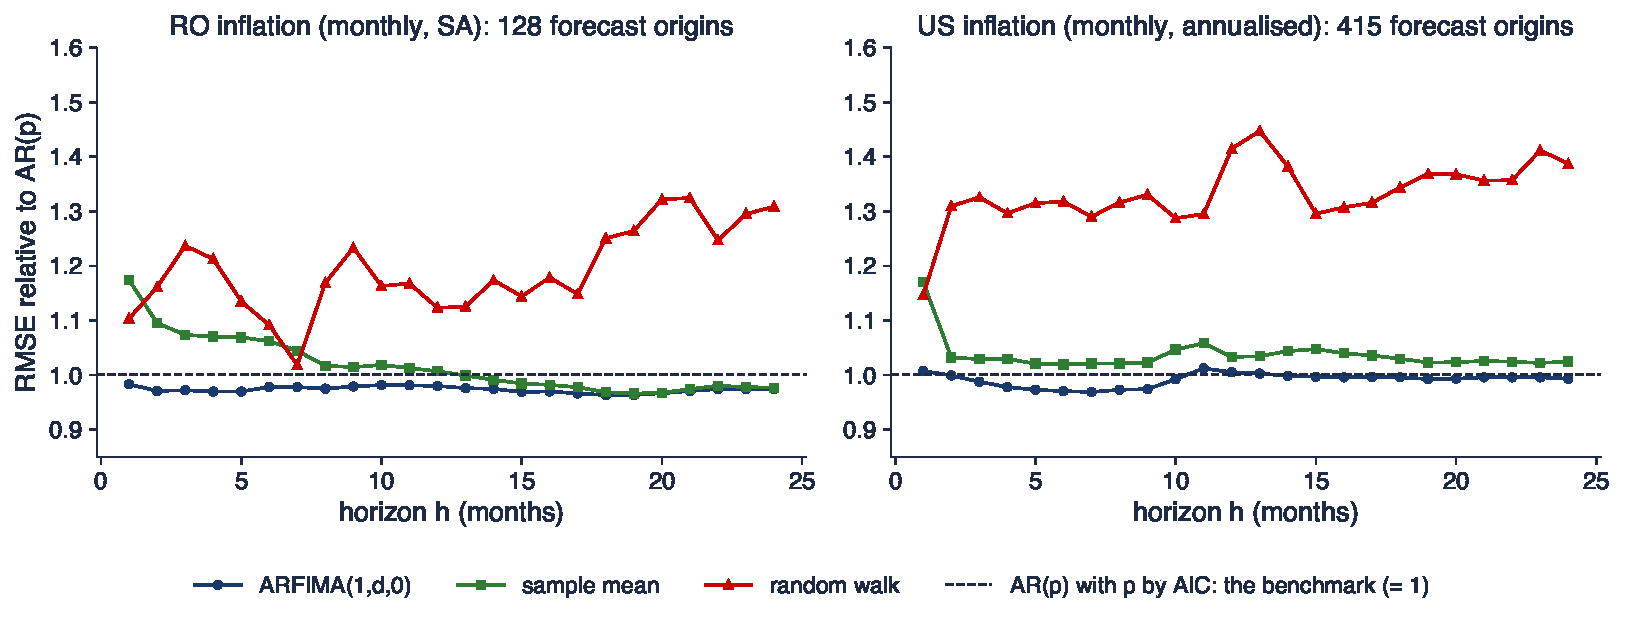
\includegraphics[width=0.97\textwidth,height=0.7\textheight,keepaspectratio]{tsa_ch8_forecast.pdf}
\end{center}
\vspace{-0.25cm}
\begin{itemize}
    \item Pseudo out-of-sample, expanding window: Romania 128 origins (January 2014--August 2024), seasonal adjustment inside each window; United States 415 origins (January 1990--July 2024). RMSE relative to AR($p$); below 1: better
\end{itemize}
\quantlet{TSA\_ch8\_forecasting}{\qlurl{TSA_ch8_forecasting}}
\end{frame}

\begin{frame}{Interpreting the forecast comparison}
\itemsize{\small}
\begin{itemize}
    \item Romania: ARFIMA beats the AR at every horizon, by 2--4\% (ratio 0.983 at 1 month, 0.980 at 12, 0.974 at 24)
    \begin{itemize}
        \item RMSE at 12 months: ARFIMA 0.53, AR 0.54, mean 0.54, random walk 0.61 (pp per month)
    \end{itemize}
    \item United States: ratios between 0.970 and 1.005: practically a tie with a rich AR($p$)
    \begin{itemize}
        \item the random walk is far worse at all horizons beyond one month
    \end{itemize}
    \item Long memory gives modest, steady gains; the large errors come from regime changes (2008, 2021--2022) that no linear model foresees; test the gains with Diebold--Mariano (\tsachlink{https://danpele.github.io/Time-Series-Analysis/EN/Courses/chapter4_seasonality_forecasting.pdf}{Chapter 4})
\end{itemize}
\end{frame}

\begin{frame}{Recap: Forecasting with ARFIMA}
\itemsize{\small}
\begin{itemize}
    \item Forecasts from the AR($\infty$) weights $\pi_k$: the whole history counts
    \item Hyperbolic return to the mean; slowly growing forecast uncertainty
    \item Inflation: small gains over AR in Romania, a tie in the United States
\end{itemize}
\end{frame}


%=============================================================================
\section{Long memory in volatility}
%=============================================================================

\begin{frame}{Case study: Ding, Granger and Engle (1993)}
\itemsize{\small}
\begin{columns}[T]
\begin{column}{0.38\textwidth}
\centering

\includegraphics[height=0.44\textheight]{ch5_robert_engle_2022.jpg}\\[1mm]
\imgcap{Robert F. Engle, Nobel Prize 2003 with Clive Granger}
\imgcredit{https://commons.wikimedia.org/wiki/File:0603-Kraneshares_KRBN-RobertEngle-JonDemske-16_(cropped).jpg}{Photo: Jon Demske (2022); CC BY-SA 4.0; Wikimedia Commons}
\end{column}
\begin{column}{0.6\textwidth}
\begin{itemize}
    \item \refDGE: daily S\&P 500 returns, 1928--1991
    \begin{itemize}
        \item returns are almost uncorrelated, but $|r_t|^\delta$ is autocorrelated for thousands of lags
        \item $\delta > 0$: a power; the autocorrelation is strongest for $\delta \approx 1$
        \item the ``long memory property'' of stock market returns: memory lives in the size, not in the sign
    \end{itemize}
    \item A GARCH(1,1) (\tsachlink{https://danpele.github.io/Time-Series-Analysis/EN/Courses/chapter5_conditional_volatility_garch.pdf}{Chapter 5}) implies autocorrelations of $r_t^2$ that fall like $(\alpha + \beta)^k$ ($\alpha$, $\beta$: the ARCH and GARCH parameters): exponentially
    \item This led to FIGARCH \refBBM\ and, with high-frequency data, to realised volatility models \refABDL, \refCorsi
\end{itemize}
\end{column}
\end{columns}
\end{frame}

\begin{frame}{Returns, absolute and squared returns}
\itemsize{\footnotesize}
\begin{center}
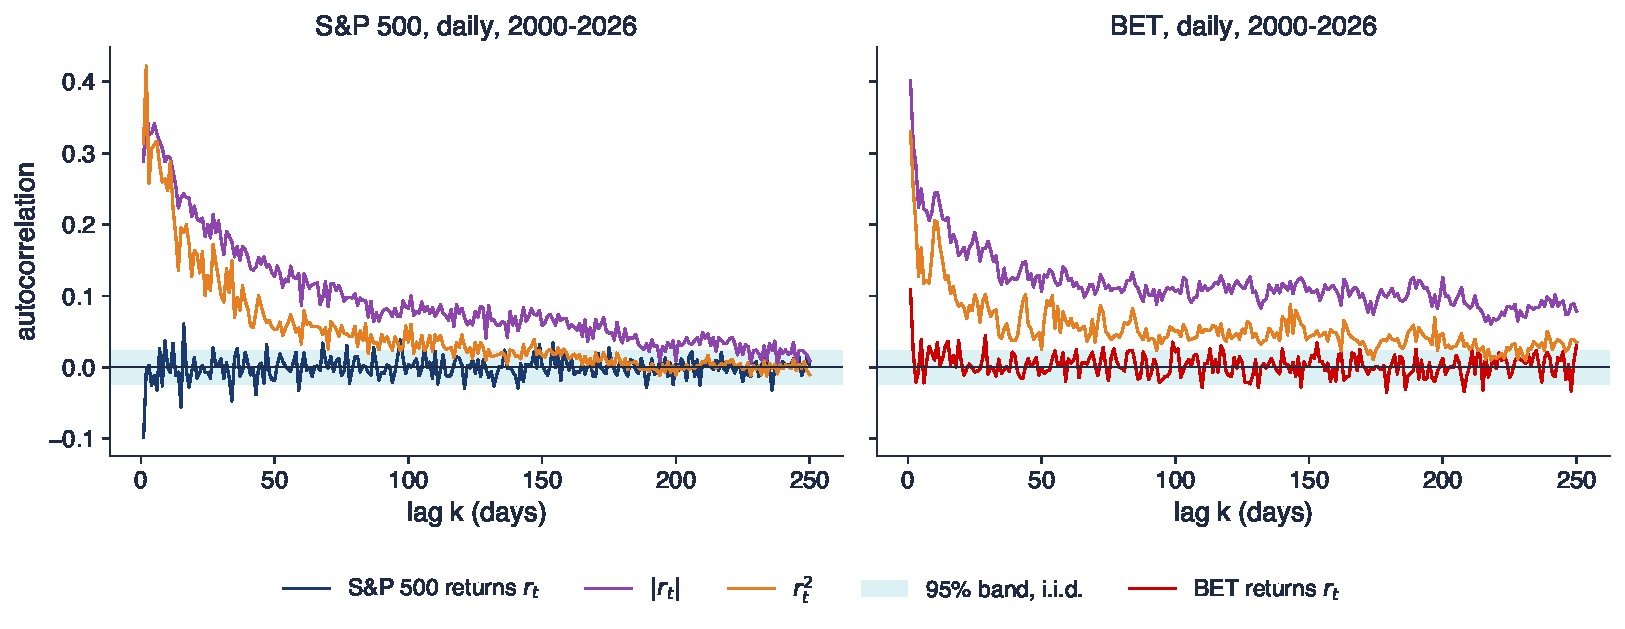
\includegraphics[width=0.97\textwidth,height=0.7\textheight,keepaspectratio]{tsa_ch8_vol_acf.pdf}
\end{center}
\vspace{-0.25cm}
\begin{itemize}
    \item Daily log returns of the S\&P 500 ($T = 6\,714$) and of the BET ($T = 6\,670$), 2000--2026; ACF up to lag 250 (one trading year); shaded: $\pm 1.96/\sqrt T$
\end{itemize}
\quantlet{TSA\_ch8\_volatility\_memory}{\qlurl{TSA_ch8_volatility_memory}}
\end{frame}

\begin{frame}{Interpreting the volatility ACF}
\itemsize{\small}
\begin{itemize}
    \item S\&P 500: $|r_t|$ has $\hat\rho = 0.29$ at lag 1 and still 0.08 at lag 100; 227 of 250 lags above the band
    \begin{itemize}
        \item BET: 0.40 at lag 1, 0.08 at lag 250, 250 of 250 above the band
    \end{itemize}
    \item $|r_t|$ is more persistent than $r_t^2$, as in \refDGE; squares are dominated by a few crash days
    \begin{itemize}
        \item local Whittle for $|r_t|$: 0.53 (S\&P 500), 0.39 (BET); after a random shuffle of the days: 0.00 and $-$0.02
    \end{itemize}
    \item The shuffle keeps the distribution and destroys the order: the memory is in the timing of calm and turbulent days, not in fat tails
\end{itemize}
\end{frame}

\begin{frame}{Realised volatility}
\itemsize{\small}
\begin{itemize}
    \item \textbf{Realised variance} of month $m$ \refABDL
    \begin{itemize}
        \item $RV_m = \sum_{t \in m} r_t^2$: the sum of the squared daily returns of the month
        \item realised volatility $\sqrt{RV_m}$ measures the volatility of month $m$ almost without a model; with intraday data the same idea gives a daily RV
    \end{itemize}
    \item We model $\log\sqrt{RV_m}$: the logarithm makes the distribution close to the Normal distribution and removes the positivity constraint
    \begin{itemize}
        \item the stylised fact of \refABDL: log RV is well described by a long-memory model with $d \approx 0.4$
    \end{itemize}
    \item Unlike $|r_t|$, $\log\sqrt{RV_m}$ is a precise measure: the noise of single days averages out within the month
\end{itemize}
\end{frame}

\begin{frame}{Monthly realised volatility: ARFIMA or ARMA?}
\itemsize{\footnotesize}
\begin{center}
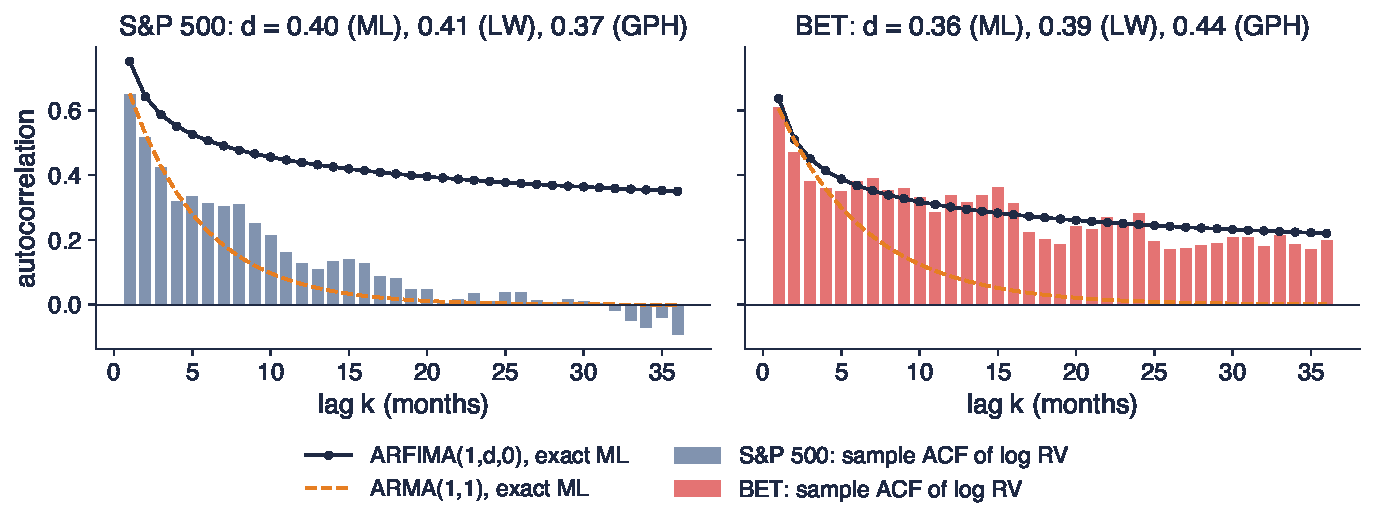
\includegraphics[width=0.97\textwidth,height=0.7\textheight,keepaspectratio]{tsa_ch8_rv.pdf}
\end{center}
\vspace{-0.25cm}
\begin{itemize}
    \item Log monthly realised volatility from daily returns, 321 months (2000--2026); lines: ACF of ARFIMA(1,$d$,0) and ARMA(1,1), both by exact ML
\end{itemize}
\quantlet{TSA\_ch8\_volatility\_memory}{\qlurl{TSA_ch8_volatility_memory}}
\end{frame}

\begin{frame}{Interpreting realised volatility}
\itemsize{\small}
\begin{itemize}
    \item All estimators agree: $d$ between 0.36 and 0.47 for both markets (ML 0.40 and 0.36)
    \begin{itemize}
        \item BET: ARFIMA fits the slow tail (lag 24: sample 0.28) and wins on BIC (343.9 against 355.4 for ARMA(1,1))
    \end{itemize}
    \item S\&P 500: the sample ACF dies out after about 20 months; ARMA(1,1) with $\phi = 0.81$ fits as well (BIC 294.4 against 295.9)
    \begin{itemize}
        \item with 27 years of data, long memory and a persistent ARMA are hard to tell apart
    \end{itemize}
    \item The sample ACF of a long-memory series is biased downwards (the sample mean absorbs part of the slow component): judge models by likelihood, not by eye
\end{itemize}
\end{frame}

\begin{frame}{FIGARCH and HAR}
\itemsize{\small}
\begin{itemize}
    \item \textbf{FIGARCH}$(1,d,1)$ \refBBM: write GARCH(1,1) as an ARMA(1,1) in $\varepsilon_t^2$ and apply $(1-L)^d$:
    \begin{itemize}
        \item $\sigma_t^2$: the conditional variance; $\varepsilon_t$: the return shock; $\omega > 0$, $\beta$, $\phi$: GARCH-type parameters (\tsachlink{https://danpele.github.io/Time-Series-Analysis/EN/Courses/chapter5_conditional_volatility_garch.pdf}{Chapter 5})
        \item $\sigma_t^2 = \omega + \beta\sigma_{t-1}^2 + \bigl[1 - \beta L - (1 - \phi L)(1-L)^d\bigr]\varepsilon_t^2 = \omega^* + \sum_{k\ge1}\lambda_k\varepsilon_{t-k}^2$
        \item $\omega^* = \omega/(1 - \beta)$; the ARCH($\infty$) weights $\lambda_k$ decay like $k^{-1-d}$; $d = 0$: GARCH, $d = 1$: IGARCH
    \end{itemize}
    \item \textbf{HAR} (heterogeneous autoregressive model) \refCorsi: $RV_{t+1} = c + \beta_d RV_t + \beta_w \overline{RV}_{t-4:t} + \beta_m \overline{RV}_{t-21:t} + u_{t+1}$
    \begin{itemize}
        \item $\overline{RV}_{t-4:t}$, $\overline{RV}_{t-21:t}$: averages over the last 5 and 22 days (weekly, monthly); $\beta_d$, $\beta_w$, $\beta_m$: their weights; estimated by OLS
        \item the idea: market participants with daily, weekly and monthly horizons
        \item not a long-memory model, but three steps that imitate a power law over the horizons that matter
    \end{itemize}
    \item Both answer the failure of GARCH from \tsachlink{https://danpele.github.io/Time-Series-Analysis/EN/Courses/chapter5_conditional_volatility_garch.pdf}{Chapter 5}: volatility shocks die out too fast in GARCH
\end{itemize}
\end{frame}

\begin{frame}{FIGARCH against GARCH; HAR against $(1-L)^d$}
\itemsize{\footnotesize}
\begin{center}
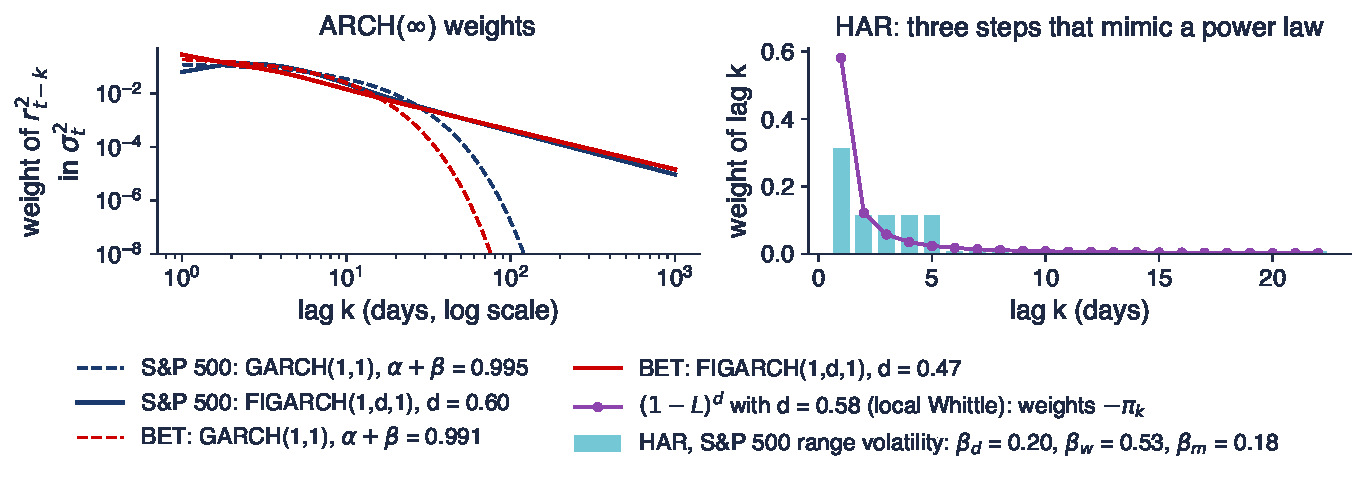
\includegraphics[width=0.97\textwidth,height=0.66\textheight,keepaspectratio]{tsa_ch8_vol_models.pdf}
\end{center}
\vspace{-0.25cm}
\begin{itemize}
    \item Left: ARCH($\infty$) weights of GARCH(1,1) and FIGARCH(1,$d$,1), Student $t$ errors, daily returns 2000--2026 (\texttt{arch})
    \item Right: HAR for the daily range-based volatility of the S\&P 500 (Parkinson estimator from high and low prices)
\end{itemize}
\quantlet{TSA\_ch8\_volatility\_memory}{\qlurl{TSA_ch8_volatility_memory}}
\end{frame}

\begin{frame}{Interpreting FIGARCH and HAR}
\itemsize{\small}
\begin{itemize}
    \item FIGARCH: $\hat d = 0.60$ (S\&P 500) and 0.47 (BET); BIC falls by 34 and 71 against GARCH
    \begin{itemize}
        \item weight of a shock 100 days ago in today's variance: GARCH $1.6 \cdot 10^{-7}$, FIGARCH $3.9 \cdot 10^{-4}$ (S\&P 500): three orders of magnitude more
    \end{itemize}
    \item GARCH reaches persistence by $\alpha + \beta = 0.995$, near 1: the near-IGARCH result of \tsachlink{https://danpele.github.io/Time-Series-Analysis/EN/Courses/chapter5_conditional_volatility_garch.pdf}{Chapter 5} is a symptom of long memory
    \begin{itemize}
        \item HAR: $\hat\beta_d = 0.20$, $\hat\beta_w = 0.53$, $\hat\beta_m = 0.18$; the weekly component dominates
    \end{itemize}
    \item The HAR steps (0.31 at lag 1, 0.11 at lags 2--5, 0.008 at lags 6--22) follow the hyperbolic weights of $(1-L)^d$ with $d = 0.58$ from local Whittle
\end{itemize}
\end{frame}

\begin{frame}{Recap: Long memory in volatility}
\itemsize{\small}
\begin{itemize}
    \item Returns: $d \approx 0$; absolute returns and realised volatility: $d \approx 0.4$
    \item The shuffle test: memory in the order of the days, not in the distribution
    \item FIGARCH: hyperbolic ARCH($\infty$) weights; HAR: a simple OLS approximation
\end{itemize}
\end{frame}


%=============================================================================
\section{Spurious long memory}
%=============================================================================

\begin{frame}{Breaks and regimes look like long memory}
\itemsize{\small}
\begin{itemize}
    \item A level shift adds a slow, step-like component: low frequencies gain power and the sample ACF decays slowly
    \begin{itemize}
        \item the same mechanism that makes a broken series look like a unit root (Perron, \tsachlink{https://danpele.github.io/Time-Series-Analysis/EN/Courses/chapter3_unit_roots_arima_models.pdf}{Chapter 3})
    \end{itemize}
    \item \refDI: a Markov-switching mean with rare switches is ``observationally equivalent'' to long memory
    \begin{itemize}
        \item the fewer the switches in a sample of length $T$, the closer the series looks to $I(d)$
        \item regime-switching models are the topic of \tsachlink{https://danpele.github.io/Time-Series-Analysis/EN/Courses/chapter10_state_space_kalman_markov_switching.pdf}{Chapter 10}
    \end{itemize}
    \item \refGH: occasional breaks explain much of the long memory of S\&P 500 absolute returns
\end{itemize}
\end{frame}

\begin{frame}{Short memory that looks long}
\itemsize{\footnotesize}
\begin{center}
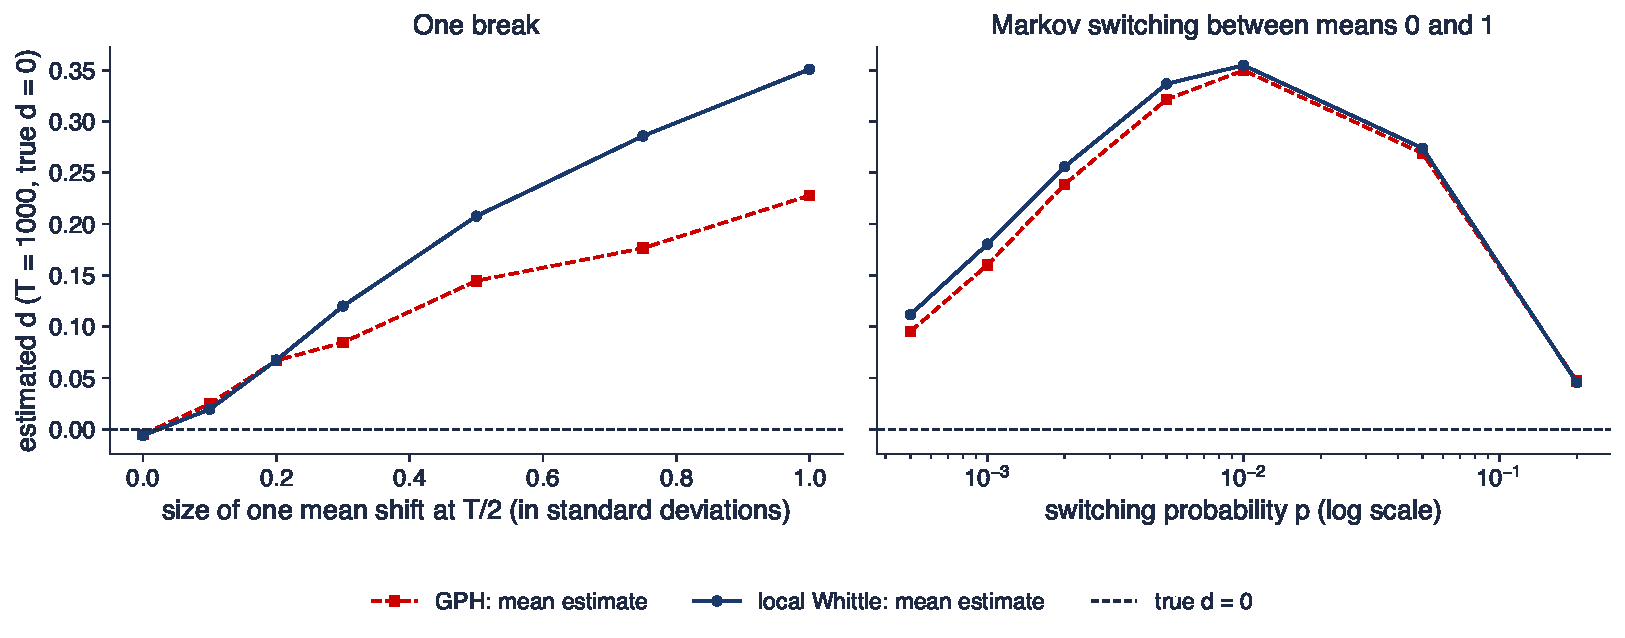
\includegraphics[width=0.97\textwidth,height=0.7\textheight,keepaspectratio]{tsa_ch8_spurious.pdf}
\end{center}
\vspace{-0.25cm}
\begin{itemize}
    \item 200 samples of $T = 1000$, true $d = 0$. Left: $N(0,1)$ noise with one mean shift at $T/2$; right: $N(0,1)$ noise plus a mean that switches between 0 and 1 with probability $p$ each period
\end{itemize}
\quantlet{TSA\_ch8\_spurious\_memory}{\qlurl{TSA_ch8_spurious_memory}}
\end{frame}

\begin{frame}{Interpreting the spurious memory}
\itemsize{\small}
\begin{itemize}
    \item One shift of half a standard deviation already gives $\hat d = 0.21$ (local Whittle); a shift of one standard deviation gives 0.35
    \begin{itemize}
        \item the break is hard to see by eye in noisy data, yet the estimator reports moderate long memory
    \end{itemize}
    \item Regime switching: with $p = 0.01$ (about 10 switches) $\hat d = 0.35$; with $p = 0.2$ (frequent switches) $\hat d = 0.05$
    \begin{itemize}
        \item rare regimes look like memory, frequent ones average out into short memory
    \end{itemize}
    \item A significant $\hat d$ is consistent with long memory and with breaks: other evidence is needed to decide
\end{itemize}
\end{frame}

\begin{frame}{The Nile in 1898: memory or a break?}
\itemsize{\footnotesize}
\begin{center}
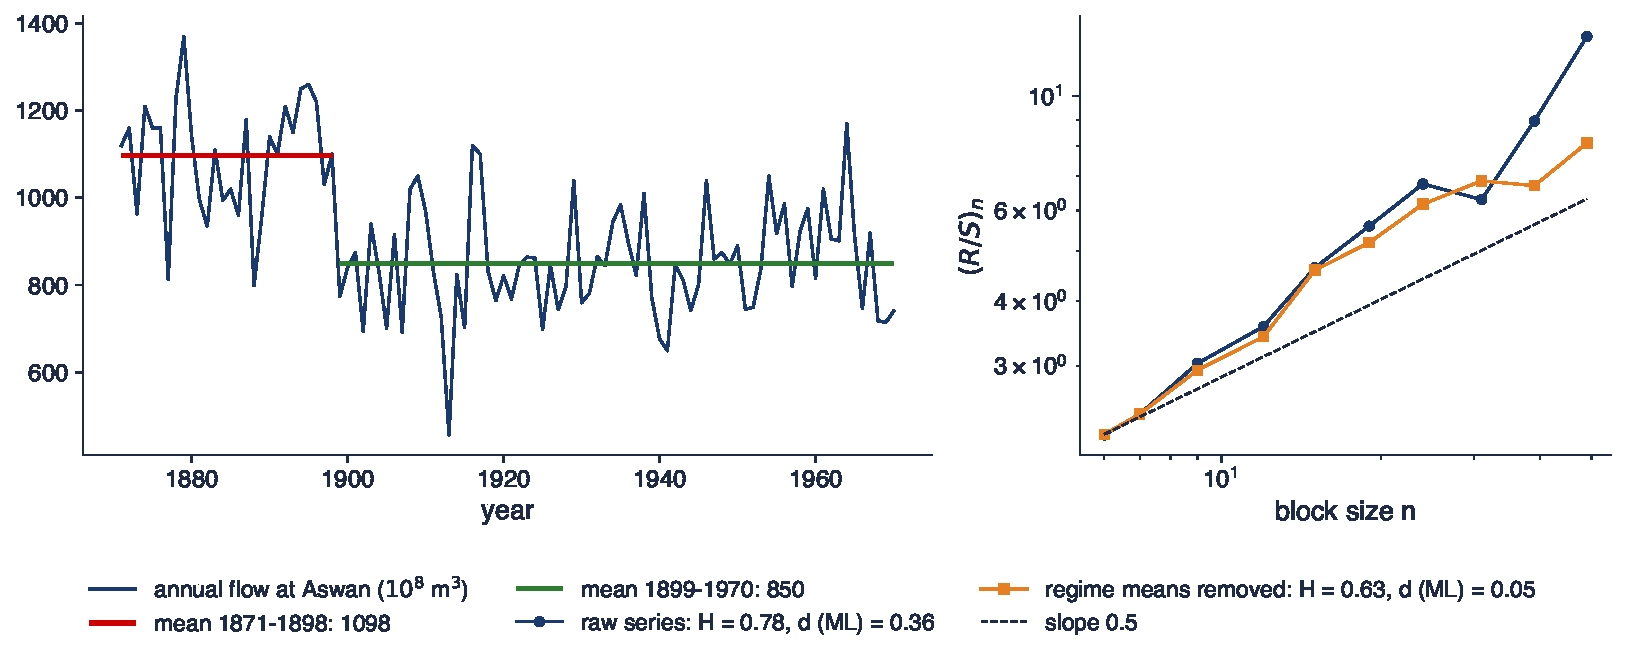
\includegraphics[width=0.97\textwidth,height=0.7\textheight,keepaspectratio]{tsa_ch8_nile_break.pdf}
\end{center}
\vspace{-0.25cm}
\begin{itemize}
    \item Left: the flow with the means before and after 1898, the change point of \refCobb{} (the first Aswan dam was completed in 1902); right: R/S plot of the raw series and of the series with the two regime means removed
\end{itemize}
\quantlet{TSA\_ch8\_spurious\_memory}{\qlurl{TSA_ch8_spurious_memory}}
\end{frame}

\begin{frame}{Interpreting the Nile break}
\itemsize{\small}
\begin{itemize}
    \item The mean falls from 1098 to 850 ($-$23\%) after 1898
    \begin{itemize}
        \item raw series: $\hat d = 0.36$ (exact ML, SE 0.07), local Whittle 0.40, R/S $H = 0.78$
    \end{itemize}
    \item Regime means removed: $\hat d = 0.05$ (SE 0.10), local Whittle $-$0.17; $\hat\rho(1)$ falls from 0.50 to 0.16
    \begin{itemize}
        \item for these 100 years one break explains almost all of the memory
    \end{itemize}
    \item Hurst's own evidence came from much longer records (the Roda gauge, from the 7th century); the lesson is to test for breaks before reading $d$
\end{itemize}
\end{frame}

\begin{frame}{The stability of memory over time}
\itemsize{\footnotesize}
\begin{center}
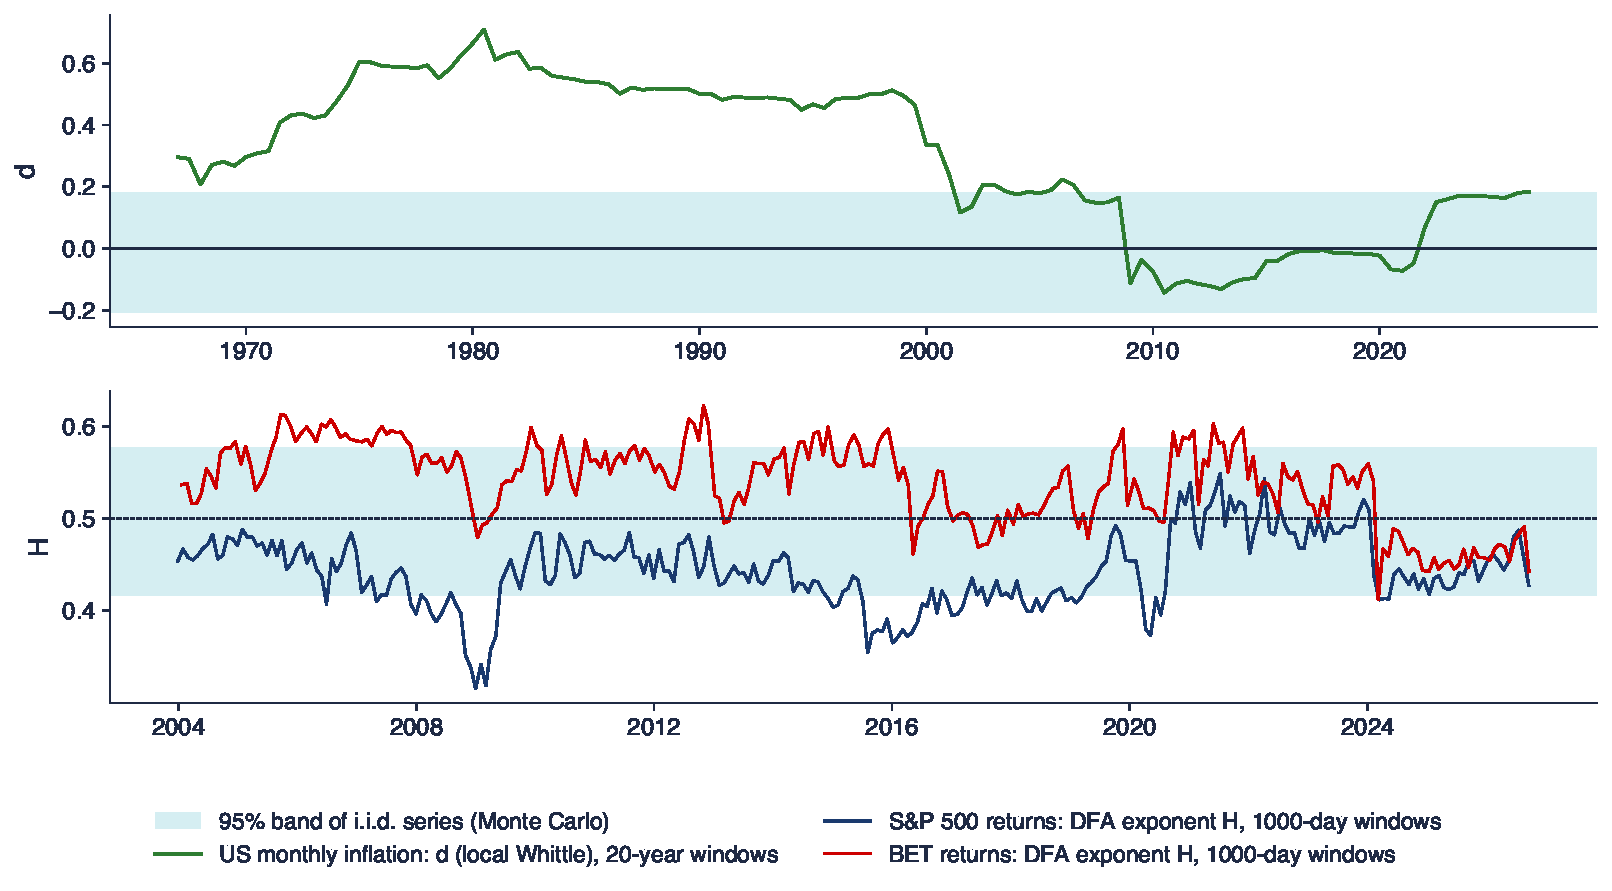
\includegraphics[width=0.97\textwidth,height=0.64\textheight,keepaspectratio]{tsa_ch8_rolling.pdf}
\end{center}
\vspace{-0.25cm}
\begin{itemize}
    \item Top: local Whittle $\hat d$ of US monthly inflation in rolling 20-year windows (dated at the window end)
    \item Bottom: DFA exponent of daily S\&P 500 and BET returns in 1000-day windows moved by 21 days; shaded: 95\% Monte Carlo bands for i.i.d. series \refWeron
\end{itemize}
\quantlet{TSA\_ch8\_spurious\_memory}{\qlurl{TSA_ch8_spurious_memory}}
\end{frame}

\begin{frame}{Interpreting the rolling estimates}
\itemsize{\small}
\begin{itemize}
    \item US inflation: $\hat d$ peaks at 0.71 in the window ending July 1980 (the Great Inflation and the Volcker disinflation) and falls to $-$0.14 (July 2010)
    \begin{itemize}
        \item in the calm years of inflation targeting $d$ is inside the band of no memory [$-$0.21, 0.18]; the 2021--2022 surge brings it back to 0.18
    \end{itemize}
    \item Returns: the S\&P 500 exponent stays mostly below 0.5 (minimum 0.32, December 2008); the BET exceeds the band in 24\% of the windows
    \begin{itemize}
        \item a less liquid market shows some persistence in returns, fading in recent years
    \end{itemize}
    \item The full-sample US estimate (0.55) mixes regimes: memory that comes and goes with monetary regimes is a sign of breaks, not of a constant $d$
\end{itemize}
\end{frame}

\begin{frame}{Checks against spurious long memory}
\itemsize{\small}
\begin{itemize}
    \item Plot the series and test for breaks (\tsachlink{https://danpele.github.io/Time-Series-Analysis/EN/Courses/chapter3_unit_roots_arima_models.pdf}{Chapter 3}: Zivot--Andrews, Bai--Perron); re-estimate $d$ on subsamples and after removing regime means
    \item Report $\hat d$ for several bandwidths $m$; a value that collapses when $m$ changes is fragile
    \item Compare ARFIMA with ARMA and with regime-switching models by likelihood and out-of-sample forecasts (\tsachlink{https://danpele.github.io/Time-Series-Analysis/EN/Courses/chapter10_state_space_kalman_markov_switching.pdf}{Chapter 10})
    \item Use the shuffle test and Monte Carlo bands built for the same sample length
    \item Avoid overlapping data (12-month inflation, rolling sums): they create artificial low-frequency power
\end{itemize}
\end{frame}

\begin{frame}{Recap: Spurious long memory}
\itemsize{\small}
\begin{itemize}
    \item Breaks and rare regime switches produce $\hat d > 0$ in short-memory series
    \item The Nile: one break in 1898 explains most of the memory of 1871--1970
    \item US inflation: $d$ changes with the monetary regime
\end{itemize}
\end{frame}


%=============================================================================
\section{A pointer: fractional cointegration}
%=============================================================================

\begin{frame}{Fractional cointegration}
\itemsize{\small}
\begin{itemize}
    \item \tsachlink{https://danpele.github.io/Time-Series-Analysis/EN/Courses/chapter7_cointegration_vecm.pdf}{Chapter 7}: two $I(1)$ series are cointegrated if a combination $y_t - \beta x_t$ is $I(0)$
    \begin{itemize}
        \item \textbf{fractional cointegration}: $x_t, y_t \sim I(d)$ and $y_t - \beta x_t \sim I(d - b)$ with $0 < b \le d$
        \item the equilibrium error may itself have long memory: deviations from equilibrium are corrected, but slowly
    \end{itemize}
    \item Example: purchasing power parity \refCL: the real exchange rate reverts to parity with $d$ between 0 and 1
    \begin{itemize}
        \item the Engle--Granger and Johansen tests of \tsachlink{https://danpele.github.io/Time-Series-Analysis/EN/Courses/chapter7_cointegration_vecm.pdf}{Chapter 7} assume $b = 1$ and may miss such slow adjustment
    \end{itemize}
    \item Beyond this course; a natural project: estimate $d$ of the residual of a cointegrating regression with local Whittle
\end{itemize}
\end{frame}


%=============================================================================
\section{Possible contribution of AI}
%=============================================================================

\begin{frame}{Possible contribution of AI}
\itemsize{\small}
\begin{itemize}
    \item \textbf{Code}: a first draft of fractional differencing, of the GPH and local Whittle estimators, of an ARFIMA likelihood
    \item \textbf{Explanation}: a second explanation of the periodogram, of the bandwidth trade-off, of the link $H = d + 1/2$
    \item \textbf{Exploration}: $d$ for many countries' inflation or many assets' volatility, with subsamples and bandwidths
    \item Example prompt
    \begin{itemize}
        \item \aiprompt{Write Python code that downloads Romanian monthly HICP (Eurostat prc\_hicp\_minr), computes the monthly inflation rate, removes the monthly means, estimates d with GPH and local Whittle for bandwidths T\^{}0.5 to T\^{}0.8, fits ARFIMA(p,d,q) by exact Gaussian maximum likelihood and compares it with ARMA(1,1) by BIC.}
    \end{itemize}
\end{itemize}
\end{frame}

\begin{frame}{Checks you must run}
\itemsize{\small}
\begin{itemize}
    \item The library: \texttt{statsmodels} has no ARFIMA class; an AI answer that calls one has invented it
    \item The sign and the scale: GPH regresses on $-\log(4\sin^2(\lambda/2))$, so the slope is $d$, not $-2d$; R/S and DFA give $H$, not $d$
    \item The range: a stationary ARFIMA likelihood needs $d < 0.5$; difference first if $\hat d$ is near or above 0.5
    \item Simulate a series with known $d$ and check that the code recovers it
    \item Breaks, seasonality and overlapping data before any claim of long memory
    \item Every cited reference: it must exist; check the DOI
\end{itemize}
\end{frame}


%=============================================================================
\section{Summary}
%=============================================================================

\begin{frame}{Key takeaways}
\itemsize{\small}
\begin{itemize}
    \item Long memory: hyperbolic ACF decay $\rho(k) \sim Ck^{2d-1}$ and a spectral pole at zero; ARMA memory is exponential
    \item $(1-L)^d$ with real $d$; ARFIMA$(p,d,q)$ separates long-run memory ($d$) from short-run dynamics (ARMA)
    \item Stationary for $d < 1/2$, invertible for $d > -1/2$, mean-reverting for $d < 1$; $H = d + 1/2$
    \item Estimate $d$ with several methods and bandwidths; prefer likelihood-based comparisons with ARMA
    \item Inflation and volatility show long memory; returns do not; breaks and regimes can fake it
\end{itemize}
\end{frame}

\begin{frame}{Key formulas}
\itemsize{\small}
{\renewcommand{\arraystretch}{1.35}\begin{center}
\footnotesize
\begin{tabular}{ll}
\toprule
\textbf{Quantity} & \textbf{Formula} \\
\midrule
ARFIMA$(p,d,q)$ & $\phi(L)(1-L)^d(x_t - \mu) = \theta(L)\varepsilon_t$ \\
Weights of $(1-L)^d$ & $\pi_0 = 1$, \quad $\pi_k = \pi_{k-1}(k - 1 - d)/k$ \\
ACF of ARFIMA$(0,d,0)$ & $\rho(1) = d/(1-d)$, \quad $\rho(k) = \rho(k-1)(k-1+d)/(k-d) \sim Ck^{2d-1}$ \\
Spectrum near 0 & $f(\lambda) \sim G\lambda^{-2d}$ \\
GPH & $\log I(\lambda_j) = c + d\,[-\log(4\sin^2(\lambda_j/2))] + u_j$, \quad SE $= \pi/\sqrt{24m}$ \\
Local Whittle & $\min_d \log\bigl(\tfrac1m\sum_j\lambda_j^{2d}I(\lambda_j)\bigr) - \tfrac{2d}{m}\sum_j\log\lambda_j$, \quad SE $= 1/(2\sqrt m)$ \\
R/S, DFA & $E(R/S)_n \approx cn^H$, \quad $F(n) \approx cn^H$, \quad $H = d + 1/2$ \\
FIGARCH & $\sigma_t^2 = \omega + \beta\sigma_{t-1}^2 + [1 - \beta L - (1 - \phi L)(1-L)^d]\varepsilon_t^2$ \\
\bottomrule
\end{tabular}
\end{center}
}
\end{frame}

\begin{frame}{Self-assessment}
\itemsize{\small}
\begin{itemize}
    \item \textbf{Question}: what are $\pi_1$ and $\pi_2$ of $(1-L)^{0.2}$?
    \begin{itemize}
        \item \textbf{Answer}: $\pi_1 = -0.2$, $\pi_2 = -0.2 \cdot 0.8/2 = -0.08$
    \end{itemize}
    \item \textbf{Question}: is ARFIMA$(0, 0.7, 0)$ stationary?
    \begin{itemize}
        \item \textbf{Answer}: no ($d \ge 0.5$), but it is mean-reverting; its first difference is ARFIMA$(0, -0.3, 0)$, stationary and anti-persistent
    \end{itemize}
    \item \textbf{Question}: GPH gives $\hat d = 0.35$ on a series with a large level shift. Is this evidence of long memory?
    \begin{itemize}
        \item \textbf{Answer}: not by itself: a break produces the same low-frequency power; re-estimate after removing the shift and on subsamples
    \end{itemize}
    \item Next: \tsachlink{https://danpele.github.io/Time-Series-Analysis/EN/Courses/chapter9_machine_learning_time_series.pdf}{Chapter 9}, machine learning for time series
\end{itemize}
\end{frame}


%=============================================================================
\section{References}
%=============================================================================

\begin{frame}{References (1/3)}
\itemsize{\scriptsize}
\begin{itemize}
    \item Andersen, T. G., Bollerslev, T., Diebold, F. X., \& Labys, P. (2003). Modeling and forecasting realized volatility. \textit{Econometrica}, 71(2), 579--625. \href{https://doi.org/10.1111/1468-0262.00418}{doi:10.1111/1468-0262.00418}
    \item Baillie, R. T. (1996). Long memory processes and fractional integration in econometrics. \textit{Journal of Econometrics}, 73(1), 5--59. \href{https://doi.org/10.1016/0304-4076(95)01732-1}{doi:10.1016/0304-4076(95)01732-1}
    \item Baillie, R. T., Bollerslev, T., \& Mikkelsen, H. O. (1996). Fractionally integrated generalized autoregressive conditional heteroskedasticity. \textit{Journal of Econometrics}, 74(1), 3--30. \href{https://doi.org/10.1016/S0304-4076(95)01749-6}{doi:10.1016/S0304-4076(95)01749-6}
    \item Beran, J., Feng, Y., Ghosh, S., \& Kulik, R. (2013). \textit{Long-Memory Processes: Probabilistic Properties and Statistical Methods}. Springer. \href{https://doi.org/10.1007/978-3-642-35512-7}{doi:10.1007/978-3-642-35512-7}
    \item Brockwell, P. J., \& Davis, R. A. (1991). \textit{Time Series: Theory and Methods} (2nd ed.). Springer. \href{https://doi.org/10.1007/978-1-4419-0320-4}{doi:10.1007/978-1-4419-0320-4}
    \item Cheung, Y.-W., \& Lai, K. S. (1993). A fractional cointegration analysis of purchasing power parity. \textit{Journal of Business \& Economic Statistics}, 11(1), 103--112. \href{https://doi.org/10.1080/07350015.1993.10509936}{doi:10.1080/07350015.1993.10509936}
    \item Cobb, G. W. (1978). The problem of the Nile: Conditional solution to a changepoint problem. \textit{Biometrika}, 65(2), 243--251. \href{https://doi.org/10.1093/biomet/65.2.243}{doi:10.1093/biomet/65.2.243}
    \item Corsi, F. (2009). A simple approximate long-memory model of realized volatility. \textit{Journal of Financial Econometrics}, 7(2), 174--196. \href{https://doi.org/10.1093/jjfinec/nbp001}{doi:10.1093/jjfinec/nbp001}
    \item Diebold, F. X., \& Inoue, A. (2001). Long memory and regime switching. \textit{Journal of Econometrics}, 105(1), 131--159. \href{https://doi.org/10.1016/S0304-4076(01)00073-2}{doi:10.1016/S0304-4076(01)00073-2}
    \item Ding, Z., Granger, C. W. J., \& Engle, R. F. (1993). A long memory property of stock market returns and a new model. \textit{Journal of Empirical Finance}, 1(1), 83--106. \href{https://doi.org/10.1016/0927-5398(93)90006-D}{doi:10.1016/0927-5398(93)90006-D}
\end{itemize}
\end{frame}

\begin{frame}{References (2/3)}
\itemsize{\scriptsize}
\begin{itemize}
    \item Fox, R., \& Taqqu, M. S. (1986). Large-sample properties of parameter estimates for strongly dependent stationary Gaussian time series. \textit{The Annals of Statistics}, 14(2), 517--532. \href{https://doi.org/10.1214/aos/1176349936}{doi:10.1214/aos/1176349936}
    \item Geweke, J., \& Porter-Hudak, S. (1983). The estimation and application of long memory time series models. \textit{Journal of Time Series Analysis}, 4(4), 221--238. \href{https://doi.org/10.1111/j.1467-9892.1983.tb00371.x}{doi:10.1111/j.1467-9892.1983.tb00371.x}
    \item Granger, C. W. J., \& Hyung, N. (2004). Occasional structural breaks and long memory with an application to the S\&P 500 absolute stock returns. \textit{Journal of Empirical Finance}, 11(3), 399--421. \href{https://doi.org/10.1016/j.jempfin.2003.03.001}{doi:10.1016/j.jempfin.2003.03.001}
    \item Granger, C. W. J., \& Joyeux, R. (1980). An introduction to long-memory time series models and fractional differencing. \textit{Journal of Time Series Analysis}, 1(1), 15--29. \href{https://doi.org/10.1111/j.1467-9892.1980.tb00297.x}{doi:10.1111/j.1467-9892.1980.tb00297.x}
    \item Graves, T., Gramacy, R., Watkins, N., \& Franzke, C. (2017). A brief history of long memory: Hurst, Mandelbrot and the road to ARFIMA, 1951--1980. \textit{Entropy}, 19(9), 437. \href{https://doi.org/10.3390/e19090437}{doi:10.3390/e19090437}
    \item Hassler, U., \& Wolters, J. (1995). Long memory in inflation rates: International evidence. \textit{Journal of Business \& Economic Statistics}, 13(1), 37--45. \href{https://doi.org/10.1080/07350015.1995.10524577}{doi:10.1080/07350015.1995.10524577}
    \item Hosking, J. R. M. (1981). Fractional differencing. \textit{Biometrika}, 68(1), 165--176. \href{https://doi.org/10.1093/biomet/68.1.165}{doi:10.1093/biomet/68.1.165}
    \item Huang, C., \& Petukhina, A. (2022). \textit{Applied Time Series Analysis and Forecasting with Python}. Springer. \href{https://doi.org/10.1007/978-3-031-13584-2}{doi:10.1007/978-3-031-13584-2}
    \item Hurst, H. E. (1951). Long-term storage capacity of reservoirs. \textit{Transactions of the American Society of Civil Engineers}, 116(1), 770--799. \href{https://doi.org/10.1061/TACEAT.0006518}{doi:10.1061/TACEAT.0006518}
\end{itemize}
\end{frame}

\begin{frame}{References (3/3)}
\itemsize{\scriptsize}
\begin{itemize}
    \item Lo, A. W. (1991). Long-term memory in stock market prices. \textit{Econometrica}, 59(5), 1279--1313. \href{https://doi.org/10.2307/2938368}{doi:10.2307/2938368}
    \item Mandelbrot, B. B., \& Van Ness, J. W. (1968). Fractional Brownian motions, fractional noises and applications. \textit{SIAM Review}, 10(4), 422--437. \href{https://doi.org/10.1137/1010093}{doi:10.1137/1010093}
    \item Mandelbrot, B. B., \& Wallis, J. R. (1968). Noah, Joseph, and operational hydrology. \textit{Water Resources Research}, 4(5), 909--918. \href{https://doi.org/10.1029/WR004i005p00909}{doi:10.1029/WR004i005p00909}
    \item Mandelbrot, B. B., \& Wallis, J. R. (1969). Robustness of the rescaled range R/S in the measurement of noncyclic long run statistical dependence. \textit{Water Resources Research}, 5(5), 967--988. \href{https://doi.org/10.1029/WR005i005p00967}{doi:10.1029/WR005i005p00967}
    \item Peng, C.-K., Buldyrev, S. V., Havlin, S., Simons, M., Stanley, H. E., \& Goldberger, A. L. (1994). Mosaic organization of DNA nucleotides. \textit{Physical Review E}, 49(2), 1685--1689. \href{https://doi.org/10.1103/PhysRevE.49.1685}{doi:10.1103/PhysRevE.49.1685}
    \item Ray, B. K. (1993). Modeling long-memory processes for optimal long-range prediction. \textit{Journal of Time Series Analysis}, 14(5), 511--525. \href{https://doi.org/10.1111/j.1467-9892.1993.tb00161.x}{doi:10.1111/j.1467-9892.1993.tb00161.x}
    \item Robinson, P. M. (1995). Gaussian semiparametric estimation of long range dependence. \textit{The Annals of Statistics}, 23(5), 1630--1661. \href{https://doi.org/10.1214/aos/1176324317}{doi:10.1214/aos/1176324317}
    \item Sowell, F. (1992). Maximum likelihood estimation of stationary univariate fractionally integrated time series models. \textit{Journal of Econometrics}, 53(1--3), 165--188. \href{https://doi.org/10.1016/0304-4076(92)90084-5}{doi:10.1016/0304-4076(92)90084-5}
    \item Velasco, C. (1999). Gaussian semiparametric estimation of non-stationary time series. \textit{Journal of Time Series Analysis}, 20(1), 87--127. \href{https://doi.org/10.1111/1467-9892.00127}{doi:10.1111/1467-9892.00127}
    \item Weron, R. (2002). Estimating long-range dependence: Finite sample properties and confidence intervals. \textit{Physica A}, 312(1--2), 285--299. \href{https://doi.org/10.1016/S0378-4371(02)00961-5}{doi:10.1016/S0378-4371(02)00961-5}
\end{itemize}
\end{frame}

\end{document}
